% Research techniques course syllabus
%
% Generate PDF-version with the following commands:
% 
% 1) latexmk -pdf "research-techniques"
% 2) biber "research-techniques"
% 3) latexmk -pdf "research-techniques"
%
\documentclass[11pt,fleqn,a4paper]{book}

%%%%%%%%%%%%%%%%%%%%%%%%%%%%%%%%%%%%%%%%%
% The Legrand Orange Book
% Structural Definitions File
% Version 2.0 (9/2/15)
%
% Original author:
% Mathias Legrand (legrand.mathias@gmail.com) with modifications by:
% Vel (vel@latextemplates.com)
%
% This file has been downloaded from:
% http://www.LaTeXTemplates.com
%
% License:
% CC BY-NC-SA 3.0 (http://creativecommons.org/licenses/by-nc-sa/3.0/)
%
%%%%%%%%%%%%%%%%%%%%%%%%%%%%%%%%%%%%%%%%%

%----------------------------------------------------------------------------------------
%	VARIOUS REQUIRED PACKAGES AND CONFIGURATIONS
%----------------------------------------------------------------------------------------

\usepackage[top=3cm,bottom=3cm,left=3cm,right=3cm,headsep=10pt,a4paper]{geometry} % Page margins

\usepackage{graphicx} % Required for including pictures
\graphicspath{{images/}} % Specifies the directory where pictures are stored

\usepackage{titling} % Macros for title, author, etc
\usepackage{lipsum} % Inserts dummy text

\usepackage{tikz} % Required for drawing custom shapes
\usepackage{pgfplotstable}
\usepackage{pgfplots}
\pgfplotsset{compat=1.13}
\usetikzlibrary{arrows,shapes,backgrounds,positioning,shadows}
\usetikzlibrary{pgfplots.statistics}


\usepackage[english]{babel} % English language/hyphenation
\usepackage{iflang}

\usepackage{paralist}
\usepackage{enumitem} % Customize lists
\setlist{nolistsep} % Reduce spacing between bullet points and numbered lists

\usepackage{booktabs} % Required for nicer horizontal rules in tables

\usepackage{xcolor} % Required for specifying colors by name
\definecolor{maincolor}{RGB}{0,100,184} % Define the main color used for highlighting throughout the book
\definecolor{hogentblue}{RGB}{0,111,184} % Define the orange color used for highlighting throughout the book

% Paragraph style: no indent, add space between paragraphs
\setlength{\parindent}{0em}
\setlength{\parskip}{1em}

%----------------------------------------------------------------------------------------
%	FONTS
%----------------------------------------------------------------------------------------

\usepackage{avant} % Use the Avantgarde font for headings
%\usepackage{times} % Use the Times font for headings
\usepackage{mathptmx} % Use the Adobe Times Roman as the default text font together with math symbols from the Sym­bol, Chancery and Com­puter Modern fonts
\usepackage{eurosym}

\usepackage{amsfonts}
\usepackage{amsmath}
\usepackage{amssymb}
\usepackage{textcomp}
\usepackage{wasysym}

\usepackage{microtype} % Slightly tweak font spacing for aesthetics
\usepackage[utf8]{inputenc} % Required for including letters with accents
\usepackage[T1]{fontenc} % Use 8-bit encoding that has 256 glyphs

%%============================================================================
%% Colours HoGent corporate identity
%%============================================================================

% Faculty colours
\definecolor{HoGentFBO}{RGB}{0,147,208} % Bedrijf en Organisatie
\definecolor{HoGentFMW}{RGB}{0,168,143} % Mens en Wetenschappen
\definecolor{HoGentFNT}{RGB}{255,0,0}   % Natuur en Techniek
\definecolor{HoGentSoA}{RGB}{0,0,0}     % School of Arts

% Accent colours
\definecolor{HoGentAccent1}{RGB}{0,111,184}   % Dark blue
\definecolor{HoGentAccent2}{RGB}{244,52,69}   % Red
\definecolor{HoGentAccent3}{RGB}{0,156,124}   % Green
\definecolor{HoGentAccent4}{RGB}{239,170,162} % Pink
\definecolor{HoGentAccent5}{RGB}{150,150,150} % Grey
\definecolor{HoGentAccent6}{RGB}{255,218,0}   % Yellow

% Aliases for accent colours
\colorlet{HoGentBlue}{HoGentAccent1}
\colorlet{HoGentRed}{HoGentAccent2}
\colorlet{HoGentGreen}{HoGentAccent3}
\colorlet{HoGentPink}{HoGentAccent4}
\colorlet{HoGentGrey}{HoGentAccent5}
\colorlet{HoGentYellow}{HoGentAccent6}

%------------------------------------------------------------------------------
%	TITLE PAGE
%------------------------------------------------------------------------------

\newcommand{\thetitlepage}{%
\begingroup
\thispagestyle{empty}
\begin{tikzpicture}[remember picture,overlay]
\coordinate [below=12cm] (midpoint) at (current page.north);
\node at (current page.north west)
{\begin{tikzpicture}[remember picture,overlay]
\node[anchor=north west,inner sep=0pt] at (0,0) {
\includegraphics[width=\paperwidth]{background}}; % Background image
\draw[anchor=north] (midpoint) node [fill=maincolor,fill opacity=0,text=white,text opacity=1,inner sep=1cm]{\Huge\centering\bfseries\sffamily\parbox[c][][t]{\paperwidth}{\centering \thetitle\\[15pt] % Book title
{\Large \thedate}\\[20pt] % Subtitle
{\large \theauthor}}}; % Author name
\end{tikzpicture}};
\end{tikzpicture}
\vfill
\endgroup
}

%----------------------------------------------------------------------------------------
%	BIBLIOGRAPHY AND INDEX
%----------------------------------------------------------------------------------------

\usepackage[style=apa,backend=biber]{biblatex}
\usepackage{csquotes}
\DeclareLanguageMapping{english}{english-apa}
\addbibresource{biblio.bib} % BibTeX bibliography file
\defbibheading{bibempty}{}

\usepackage{calc} % For simpler calculation - used for spacing the index letter headings correctly
\usepackage{makeidx} % Required to make an index
\makeindex % Tells LaTeX to create the files required for indexing

%----------------------------------------------------------------------------------------
%	MAIN TABLE OF CONTENTS
%----------------------------------------------------------------------------------------

\usepackage{titletoc} % Required for manipulating the table of contents

\contentsmargin{0cm} % Removes the default margin

% Part text styling
\titlecontents{part}[0cm]
{\addvspace{20pt}\centering\large\bfseries}
{}
{}
{}

% Chapter text styling
\titlecontents{chapter}[1.25cm] % Indentation
{\addvspace{12pt}\large\sffamily\bfseries} % Spacing and font options for chapters
{\color{maincolor!60}\contentslabel[\Large\thecontentslabel]{1.25cm}\color{maincolor}} % Chapter number
{\color{maincolor}}
{\color{maincolor!60}\normalsize\;\titlerule*[.5pc]{.}\;\thecontentspage} % Page number

% Section text styling
\titlecontents{section}[1.25cm] % Indentation
{\addvspace{3pt}\sffamily\bfseries} % Spacing and font options for sections
{\contentslabel[\thecontentslabel]{1.25cm}} % Section number
{}
{\hfill\color{black}\thecontentspage} % Page number
[]

% Subsection text styling
\titlecontents{subsection}[1.25cm] % Indentation
{\addvspace{1pt}\sffamily\small} % Spacing and font options for subsections
{\contentslabel[\thecontentslabel]{1.25cm}} % Subsection number
{}
{\ \titlerule*[.5pc]{.}\;\thecontentspage} % Page number
[]

% List of figures
\titlecontents{figure}[0em]
{\addvspace{-5pt}\sffamily}
{\thecontentslabel\hspace*{1em}}
{}
{\ \titlerule*[.5pc]{.}\;\thecontentspage}
[]

% List of tables
\titlecontents{table}[0em]
{\addvspace{-5pt}\sffamily}
{\thecontentslabel\hspace*{1em}}
{}
{\ \titlerule*[.5pc]{.}\;\thecontentspage}
[]

%----------------------------------------------------------------------------------------
%	MINI TABLE OF CONTENTS IN PART HEADS
%----------------------------------------------------------------------------------------

% Chapter text styling
\titlecontents{lchapter}[0em] % Indenting
{\addvspace{15pt}\large\sffamily\bfseries} % Spacing and font options for chapters
{\color{maincolor}\contentslabel[\Large\thecontentslabel]{1.25cm}\color{maincolor}} % Chapter number
{}
{\color{maincolor}\normalsize\sffamily\bfseries\;\titlerule*[.5pc]{.}\;\thecontentspage} % Page number

% Section text styling
\titlecontents{lsection}[0em] % Indenting
{\sffamily\small} % Spacing and font options for sections
{\contentslabel[\thecontentslabel]{1.25cm}} % Section number
{}
{}

% Subsection text styling
\titlecontents{lsubsection}[.5em] % Indentation
{\normalfont\footnotesize\sffamily} % Font settings
{}
{}
{}

%----------------------------------------------------------------------------------------
%	PAGE HEADERS
%----------------------------------------------------------------------------------------

\usepackage{fancyhdr} % Required for header and footer configuration

\pagestyle{fancy}
\renewcommand{\chaptermark}[1]{\markboth{\sffamily\normalsize\bfseries\chaptername\ \thechapter.\ #1}{}} % Chapter text font settings
\renewcommand{\sectionmark}[1]{\markright{\sffamily\normalsize\thesection\hspace{5pt}#1}{}} % Section text font settings
\fancyhf{} \fancyhead[LE,RO]{\sffamily\normalsize\thepage} % Font setting for the page number in the header
\fancyhead[LO]{\rightmark} % Print the nearest section name on the left side of odd pages
\fancyhead[RE]{\leftmark} % Print the current chapter name on the right side of even pages
\renewcommand{\headrulewidth}{0.5pt} % Width of the rule under the header
\addtolength{\headheight}{2.5pt} % Increase the spacing around the header slightly
\renewcommand{\footrulewidth}{0pt} % Removes the rule in the footer
\fancypagestyle{plain}{\fancyhead{}\renewcommand{\headrulewidth}{0pt}} % Style for when a plain pagestyle is specified

% Removes the header from odd empty pages at the end of chapters
\makeatletter
\renewcommand{\cleardoublepage}{
\clearpage\ifodd\c@page\else
\hbox{}
\vspace*{\fill}
\thispagestyle{empty}
\newpage
\fi}

%----------------------------------------------------------------------------------------
%	THEOREM STYLES
%----------------------------------------------------------------------------------------

\usepackage{amsmath,amsfonts,amssymb,amsthm} % For math equations, theorems, symbols, etc

\newcommand{\intoo}[2]{\mathopen{]}#1\,;#2\mathclose{[}}
\newcommand{\ud}{\mathop{\mathrm{{}d}}\mathopen{}}
\newcommand{\intff}[2]{\mathopen{[}#1\,;#2\mathclose{]}}
\newtheorem{notation}{Notation}[chapter]

% Boxed/framed environments
\newtheoremstyle{maincolornumbox}% % Theorem style name
{0pt}% Space above
{0pt}% Space below
{\normalfont}% % Body font
{}% Indent amount
{\small\bf\sffamily\color{maincolor}}% % Theorem head font
{\;}% Punctuation after theorem head
{0.25em}% Space after theorem head
{\small\sffamily\color{maincolor}\thmname{#1}\nobreakspace\thmnumber{\@ifnotempty{#1}{}\@upn{#2}}% Theorem text (e.g. Theorem 2.1)
\thmnote{\nobreakspace\the\thm@notefont\sffamily\bfseries\color{black}---\nobreakspace#3.}} % Optional theorem note
\renewcommand{\qedsymbol}{$\blacksquare$}% Optional qed square

\newtheoremstyle{blacknumex}% Theorem style name
{5pt}% Space above
{5pt}% Space below
{\normalfont}% Body font
{} % Indent amount
{\small\bf\sffamily}% Theorem head font
{\;}% Punctuation after theorem head
{0.25em}% Space after theorem head
{\small\sffamily{\tiny\ensuremath{\blacksquare}}\nobreakspace\thmname{#1}\nobreakspace\thmnumber{\@ifnotempty{#1}{}\@upn{#2}}% Theorem text (e.g. Theorem 2.1)
\thmnote{\nobreakspace\the\thm@notefont\sffamily\bfseries---\nobreakspace#3.}}% Optional theorem note

\newtheoremstyle{blacknumbox} % Theorem style name
{0pt}% Space above
{0pt}% Space below
{\normalfont}% Body font
{}% Indent amount
{\small\bf\sffamily}% Theorem head font
{\;}% Punctuation after theorem head
{0.25em}% Space after theorem head
{\small\sffamily\thmname{#1}\nobreakspace\thmnumber{\@ifnotempty{#1}{}\@upn{#2}}% Theorem text (e.g. Theorem 2.1)
\thmnote{\nobreakspace\the\thm@notefont\sffamily\bfseries---\nobreakspace#3.}}% Optional theorem note

% Non-boxed/non-framed environments
\newtheoremstyle{maincolornum}% % Theorem style name
{5pt}% Space above
{5pt}% Space below
{\normalfont}% % Body font
{}% Indent amount
{\small\bf\sffamily\color{maincolor}}% % Theorem head font
{\;}% Punctuation after theorem head
{0.25em}% Space after theorem head
{\small\sffamily\color{maincolor}\thmname{#1}\nobreakspace\thmnumber{\@ifnotempty{#1}{}\@upn{#2}}% Theorem text (e.g. Theorem 2.1)
\thmnote{\nobreakspace\the\thm@notefont\sffamily\bfseries\color{black}---\nobreakspace#3.}} % Optional theorem note
\renewcommand{\qedsymbol}{$\blacksquare$}% Optional qed square
\makeatother

%----------------------------------------------------------------------------------------
%	DEFINITION OF COLORED BOXES
%----------------------------------------------------------------------------------------

\RequirePackage[framemethod=default]{mdframed} % Required for creating the theorem, definition, exercise and corollary boxes

\newcounter{dummy} 
\newtheorem{theoremeT}[dummy]{Theorem}
\newtheorem{problem}{Problem}[chapter]
\newtheorem{exerciseT}{Exercise}[chapter]
\newtheorem{exampleT}{Example}[chapter]
\newtheorem{definitionT}{Definition}[section]

% Theorem box
\newmdenv[skipabove=7pt,
skipbelow=7pt,
backgroundcolor=black!5,
linecolor=maincolor,
innerleftmargin=5pt,
innerrightmargin=5pt,
innertopmargin=7pt,
innerbottommargin=7pt,
leftmargin=0cm,
rightmargin=0cm,
innerbottommargin=5pt]{tBox}

% Exercise box
\newmdenv[skipabove=7pt,
skipbelow=7pt,
rightline=false,
leftline=true,
topline=false,
bottomline=false,
backgroundcolor=maincolor!10,
linecolor=maincolor,
innerleftmargin=5pt,
innerrightmargin=5pt,
innertopmargin=7pt,
innerbottommargin=7pt,
leftmargin=0cm,
rightmargin=0cm,
linewidth=4pt]{eBox}

% Definition box
\newmdenv[skipabove=7pt,
skipbelow=7pt,
rightline=false,
leftline=true,
topline=false,
bottomline=false,
linecolor=maincolor,
innerleftmargin=5pt,
innerrightmargin=5pt,
innertopmargin=7pt,
innerbottommargin=7pt,
leftmargin=0cm,
rightmargin=0cm,
linewidth=4pt,
innerbottommargin=0pt]{dBox}

% Corollary box
\newmdenv[skipabove=7pt,
skipbelow=7pt,
rightline=false,
leftline=true,
topline=false,
bottomline=false,
linecolor=gray,
backgroundcolor=black!5,
innerleftmargin=5pt,
innerrightmargin=5pt,
innertopmargin=7pt,
innerbottommargin=7pt,
leftmargin=0cm,
rightmargin=0cm,
linewidth=4pt,
innerbottommargin=5pt]{cBox}

% Creates an environment for each type of theorem and assigns it a theorem text style from the "Theorem Styles" section above and a colored box from above
\newenvironment{theorem}{\begin{tBox}\begin{theoremeT}}{\end{theoremeT}\end{tBox}}
\newenvironment{exercise}{\begin{eBox}\begin{exerciseT}}{\hfill{\color{maincolor}\tiny\ensuremath{\blacksquare}}\end{exerciseT}\end{eBox}}
\newenvironment{definition}{\begin{dBox}\begin{definitionT}}{\end{definitionT}\end{dBox}}
\newenvironment{example}{\begin{exampleT}}{\hfill{\tiny\ensuremath{\blacksquare}}\end{exampleT}}
\newenvironment{corollary}{\begin{cBox}\begin{corollaryT}}{\end{corollaryT}\end{cBox}}

%----------------------------------------------------------------------------------------
%	REMARK ENVIRONMENT
%----------------------------------------------------------------------------------------

\newenvironment{remark}{\par\vspace{10pt}\small % Vertical white space above the remark and smaller font size
\begin{list}{}{
\leftmargin=35pt % Indentation on the left
\rightmargin=25pt}\item\ignorespaces % Indentation on the right
\makebox[-2.5pt]{\begin{tikzpicture}[overlay]
\node[draw=maincolor!60,line width=1pt,circle,fill=maincolor!25,font=\sffamily\bfseries,inner sep=2pt,outer sep=0pt] at (-15pt,0pt){\textcolor{maincolor}{R}};\end{tikzpicture}} % Orange R in a circle
\advance\baselineskip -1pt}{\end{list}\vskip5pt} % Tighter line spacing and white space after remark

%----------------------------------------------------------------------------------------
%	SECTION NUMBERING IN THE MARGIN
%----------------------------------------------------------------------------------------

\makeatletter
\renewcommand{\@seccntformat}[1]{\llap{\textcolor{maincolor}{\csname the#1\endcsname}\hspace{1em}}}
\renewcommand{\section}{\@startsection{section}{1}{\z@}
{-4ex \@plus -1ex \@minus -.4ex}
{1ex \@plus.2ex }
{\normalfont\large\sffamily\bfseries}}
\renewcommand{\subsection}{\@startsection {subsection}{2}{\z@}
{-3ex \@plus -0.1ex \@minus -.4ex}
{0.5ex \@plus.2ex }
{\normalfont\sffamily\bfseries}}
\renewcommand{\subsubsection}{\@startsection {subsubsection}{3}{\z@}
{-2ex \@plus -0.1ex \@minus -.2ex}
{.2ex \@plus.2ex }
{\normalfont\small\sffamily\bfseries}}
\renewcommand\paragraph{\@startsection{paragraph}{4}{\z@}
{-2ex \@plus-.2ex \@minus .2ex}
{.1ex}
{\normalfont\small\sffamily\bfseries}}

%----------------------------------------------------------------------------------------
%	PART HEADINGS
%----------------------------------------------------------------------------------------

% numbered part in the table of contents
\newcommand{\@mypartnumtocformat}[2]{%
\setlength\fboxsep{0pt}%
\noindent\colorbox{maincolor!20}{\strut\parbox[c][.7cm]{\ecart}{\color{maincolor!70}\Large\sffamily\bfseries\centering#1}}\hskip\esp\colorbox{maincolor!40}{\strut\parbox[c][.7cm]{\linewidth-\ecart-\esp}{\Large\sffamily\centering#2}}}%
%%%%%%%%%%%%%%%%%%%%%%%%%%%%%%%%%%
% unnumbered part in the table of contents
\newcommand{\@myparttocformat}[1]{%
\setlength\fboxsep{0pt}%
\noindent\colorbox{maincolor!40}{\strut\parbox[c][.7cm]{\linewidth}{\Large\sffamily\centering#1}}}%
%%%%%%%%%%%%%%%%%%%%%%%%%%%%%%%%%%
\newlength\esp
\setlength\esp{4pt}
\newlength\ecart
\setlength\ecart{1.2cm-\esp}
\newcommand{\thepartimage}{}%
\newcommand{\partimage}[1]{\renewcommand{\thepartimage}{#1}}%
\def\@part[#1]#2{%
\ifnum \c@secnumdepth >-2\relax%
\refstepcounter{part}%
\addcontentsline{toc}{part}{\texorpdfstring{\protect\@mypartnumtocformat{\thepart}{#1}}{\partname~\thepart\ ---\ #1}}
\else%
\addcontentsline{toc}{part}{\texorpdfstring{\protect\@myparttocformat{#1}}{#1}}%
\fi%
\startcontents%
\markboth{}{}%
{\thispagestyle{empty}%
\begin{tikzpicture}[remember picture,overlay]%
\node at (current page.north west){\begin{tikzpicture}[remember picture,overlay]%
\fill[maincolor!20](0cm,0cm) rectangle (\paperwidth,-\paperheight);
\node[anchor=north] at (4cm,-3.25cm){\color{maincolor!40}\fontsize{220}{100}\sffamily\bfseries\@Roman\c@part};
\node[anchor=south east] at (\paperwidth-1cm,-\paperheight+1cm){\parbox[t][][t]{8.5cm}{
\printcontents{l}{0}{\setcounter{tocdepth}{1}}%
}};
\node[anchor=north east] at (\paperwidth-1.5cm,-3.25cm){\parbox[t][][t]{15cm}{\strut\raggedleft\color{white}\fontsize{30}{30}\sffamily\bfseries#2}};
\end{tikzpicture}};
\end{tikzpicture}}%
\@endpart}
\def\@spart#1{%
\startcontents%
\phantomsection
{\thispagestyle{empty}%
\begin{tikzpicture}[remember picture,overlay]%
\node at (current page.north west){\begin{tikzpicture}[remember picture,overlay]%
\fill[maincolor!20](0cm,0cm) rectangle (\paperwidth,-\paperheight);
\node[anchor=north east] at (\paperwidth-1.5cm,-3.25cm){\parbox[t][][t]{15cm}{\strut\raggedleft\color{white}\fontsize{30}{30}\sffamily\bfseries#1}};
\end{tikzpicture}};
\end{tikzpicture}}
\addcontentsline{toc}{part}{\texorpdfstring{%
\setlength\fboxsep{0pt}%
\noindent\protect\colorbox{maincolor!40}{\strut\protect\parbox[c][.7cm]{\linewidth}{\Large\sffamily\protect\centering #1\quad\mbox{}}}}{#1}}%
\@endpart}
\def\@endpart{\vfil\newpage
\if@twoside
\if@openright
\null
\thispagestyle{empty}%
\newpage
\fi
\fi
\if@tempswa
\twocolumn
\fi}

%----------------------------------------------------------------------------------------
%	CHAPTER HEADINGS
%----------------------------------------------------------------------------------------

% A switch to conditionally include a picture, implemented by  Christian Hupfer
\newif\ifusechapterimage
\usechapterimagetrue
\newcommand{\thechapterimage}{}%
\newcommand{\chapterimage}[1]{\ifusechapterimage\renewcommand{\thechapterimage}{#1}\fi}%
\def\@makechapterhead#1{%
{\parindent \z@ \raggedright \normalfont
\ifnum \c@secnumdepth >\m@ne
\if@mainmatter
\begin{tikzpicture}[remember picture,overlay]
\node at (current page.north west)
{\begin{tikzpicture}[remember picture,overlay]
\node[anchor=north west,inner sep=0pt] at (0,0) {\ifusechapterimage\includegraphics[width=\paperwidth]{\thechapterimage}\fi};
\draw[anchor=west] (\Gm@lmargin,-9cm) node [line width=2pt,rounded corners=15pt,draw=maincolor,fill=white,fill opacity=0.5,inner sep=15pt]{\strut\makebox[22cm]{}};
\draw[anchor=west] (\Gm@lmargin+.3cm,-9cm) node {\huge\sffamily\bfseries\color{black}\thechapter. #1\strut};
\end{tikzpicture}};
\end{tikzpicture}
\else
\begin{tikzpicture}[remember picture,overlay]
\node at (current page.north west)
{\begin{tikzpicture}[remember picture,overlay]
\node[anchor=north west,inner sep=0pt] at (0,0) {\ifusechapterimage\includegraphics[width=\paperwidth]{\thechapterimage}\fi};
\draw[anchor=west] (\Gm@lmargin,-9cm) node [line width=2pt,rounded corners=15pt,draw=maincolor,fill=white,fill opacity=0.5,inner sep=15pt]{\strut\makebox[22cm]{}};
\draw[anchor=west] (\Gm@lmargin+.3cm,-9cm) node {\huge\sffamily\bfseries\color{black}#1\strut};
\end{tikzpicture}};
\end{tikzpicture}
\fi\fi\par\vspace*{270\p@}}}

%-------------------------------------------

\def\@makeschapterhead#1{%
\begin{tikzpicture}[remember picture,overlay]
\node at (current page.north west)
{\begin{tikzpicture}[remember picture,overlay]
\node[anchor=north west,inner sep=0pt] at (0,0) {\ifusechapterimage\includegraphics[width=\paperwidth]{\thechapterimage}\fi};
\draw[anchor=west] (\Gm@lmargin,-9cm) node [line width=2pt,rounded corners=15pt,draw=maincolor,fill=white,fill opacity=0.5,inner sep=15pt]{\strut\makebox[22cm]{}};
\draw[anchor=west] (\Gm@lmargin+.3cm,-9cm) node {\huge\sffamily\bfseries\color{black}#1\strut};
\end{tikzpicture}};
\end{tikzpicture}
\par\vspace*{270\p@}}
\makeatother

%----------------------------------------------------------------------------------------
%	HYPERLINKS IN THE DOCUMENTS
%----------------------------------------------------------------------------------------

\usepackage{hyperref}
\hypersetup{hidelinks,colorlinks=false,breaklinks=true,urlcolor= maincolor,bookmarksopen=false,pdftitle={Title},pdfauthor={Author}}
\usepackage{bookmark}
\bookmarksetup{
open,
numbered,
addtohook={%
\ifnum\bookmarkget{level}=0 % chapter
\bookmarksetup{bold}%
\fi
\ifnum\bookmarkget{level}=-1 % part
\bookmarksetup{color=maincolor,bold}%
\fi
}
}

%----------------------------------------------------------------------------------------
%	Math stuff
%----------------------------------------------------------------------------------------

\pgfmathdeclarefunction{gauss}{2}{%
	\pgfmathparse{1/(#2*sqrt(2*pi))*exp(-((x-#1)^2)/(2*#2^2))}%
}

\def\R{\mathbb{R}}


%----------------------------------------------------------------------------------------
%	Format R code
%----------------------------------------------------------------------------------------
\usepackage{listings}

\lstset{ %
  language=R,                     % the language of the code
  inputencoding=utf8,             % Allow (some) Unicode characters in the code
  extendedchars=true,
  literate={é}{{\'e}}1 {ë}{{\"e}}1 {è}{{\`e}}1 {á}{{\'a}}1 {à}{{\`a}}1 {ó}{{\'o}}1 {ò}{{\`o}}1 {²}{{$^2$}}1 {€}{{\euro}}1,
  basicstyle=\normalsize,       % the size of the fonts that are used for the code
  numbers=left,                   % where to put the line-numbers
  numberstyle=\tiny\color{gray},  % the style that is used for the line-numbers
  stepnumber=1,                   % the step between two line-numbers. If it's 1, each line
  % will be numbered
  numbersep=5pt,                  % how far the line-numbers are from the code
  backgroundcolor=\color{white},  % choose the background color. You must add \usepackage{color}
  showspaces=false,               % show spaces adding particular underscores
  showstringspaces=false,         % underline spaces within strings
  showtabs=false,                 % show tabs within strings adding particular underscores
  frame=single,                   % adds a frame around the code
  rulecolor=\color{black},        % if not set, the frame-color may be changed on line-breaks within not-black text (e.g. commens (green here))
  tabsize=2,                      % sets default tabsize to 2 spaces
  captionpos=b,                   % sets the caption-position to bottom
  breaklines=true,                % sets automatic line breaking
  breakatwhitespace=false,        % sets if automatic breaks should only happen at whitespace
  keywordstyle=\color{HoGentBlue},      % keyword style
  commentstyle=\color{HoGentGrey},   % comment style
  stringstyle=\color{HoGentRed},      % string literal style
  escapeinside={\%*}{*)},         % if you want to add a comment within your code
  morekeywords={*,...}            % if you want to add more keywords to the set
}

\author{Dr. Jens Buysse, Anita Bernard, Bert Van Vreckem}
\title{Research Techniques}
\date{Academic year 2016-2017}

\begin{document}

\thetitlepage

%----------------------------------------------------------------------------------------
%	COPYRIGHT PAGE
%----------------------------------------------------------------------------------------

\newpage
~\vfill
\thispagestyle{empty}

\noindent Copyright \copyright\ 2015-2017 Jens Buysse\\ % Copyright notice

\noindent English translation by Bert Van Vreckem\\

\noindent \textsc{www.hogent.be}\\ % URL

\noindent \textit{Generated on \today} % Printing/edition date

%----------------------------------------------------------------------------------------
%	TABLE OF CONTENTS
%----------------------------------------------------------------------------------------

\usechapterimagefalse

\tableofcontents % Print the table of contents itself

\cleardoublepage % Forces the first chapter to start on an odd page so it's on the right

\setlength{\parindent}{0pt}

\def\R{\mathbb{R}}

%

\chapter*{Acknowledgements}

This syllabus was written for the Research Techniques course in the Bachelor programme Applied Informatics at University College Ghent. I'd like to take the opportunity to thank the following people for suggesting improvements for this course.

\begin{itemize}
	\item C\'edric Berlez
	\item J\"urgen Van Meerhaeghe
	\item Gianni Stubbe
	\item Jelle Elaut
	\item Thijs Van Der Burgt
	\item Lotte Potth\'e
	\item \"Ozg\"ur Akin
\end{itemize}

\bigskip \bigskip
{\raggedleft%
Jens Buysse\\
February 8, 2016\\
}

\chapter{The research process}
\section{The scientific method}

There are several ways to gather knowledge:

\begin{enumerate}
	\item The non-scientific method
	\item The scientific method
\end{enumerate}

\paragraph{Non-scientific} Several versions of non-scientific reasoning exist:
\begin{description}
	\item [Authoritarian] Someone is considered to be an authority on a certain subject and to be trustworthy. Every claim this person makes is regarded as the truth.
	\item [Deductive] Given a set of assumptions, logical reasoning leads to certain conclusions. This way, correct results \emph{may} be found, but these depend solely on the truth of the assumptions. These are not researched empirically, though.
\end{description}

\paragraph{Scientific} A characteristic of the scientific method is \textbf{empiricall validation}: based on experience and direct observation. A claim is only valid if it corresponds to what is observed.

\begin{exercise}
Try to prove that pigs can fly, starting from both a non-scientific and a scientific reasoning.
\end{exercise}

Empirical research may have several goals:

\begin{description}
    \item[Exploration] Does something exist, or does a certain event occur?
    \item[Description] What are the properties of this event?
    \item[Prediction] Is a certain event related to another one and is it possible to predict it?
    \item[Verification] Is it possible to completely predect a certain event based on other observations?
\end{description}

\paragraph{Research objectives}

Most research objectives can be categorised into:

\begin{description}
	\item[Generalisation] Often research is conducted on a limited \emph{sample} of the group that is being studied, the \emph{population}. If conclusions for this sample also hold for the population, we have found a valid generalisation.
    \item[Specialisation] Applying general knowledge to specific instances or domains. A lot of applied research can be classified under this category.
\end{description}

Two types of generalisation are discerned:

\begin{enumerate}
	\item About a single phenomenon;
	\item About relations between phenomena.
\end{enumerate}

There are three reasons why relations between phenomena are so important:

\begin{enumerate}
	\item A complete understanding of the phenomenon;
	\item Relations may enable prediction;
	\item Revealing causal relations.
\end{enumerate}

\begin{definition}[Causal relation]
    Two variables have a \emph{causal relation} when a change in the first variable reliably causes an associated change into the second one, provided that all other potential causes are eliminated. The first variable is called the \emph{independent variable}, the second the \emph{dependent variable}.
\end{definition}

\section{Basic concepts in research}

\paragraph{Levels of measurement}

In quantitative research, we try to comprehend a phenomenon by measuring it.

\begin{definition}[Variable]
     A general property of an object that allows us to distinguish it. E.g.~length, mass, etc.
\end{definition}

\begin{definition}[Value]
    The specific property of a specific object. The measurement assigned to a variable. E.g.~1.83m, 78kg, etc.
\end{definition}

In statistical analysis, a classification of variable types is used that helps determining which statistical methods can be applied to the variable in question. A common taxonomy of the level of measurement is:

\begin{description}
	\item [Nominal] The variable can only take a limited number of values, and there is no logical order between them. E.g.~gender, nationality, biological species, etc.
	\item [Ordinal] The variable can take a limited number of values, but there is a logical ordering between them. E.g.~Likert scale when measuring opinion (from \emph{strongly disagree} to \emph{strongly agree}), military rank, etc.
	\item [Interval] A numerical variable that allows for the degree of difference between items, but not the ratio between them. There is no meaningful zero value. E.g.~temperature.
	\item [Ratio] A numerical variable with a non-arbitrary zero point, that allows for meaningful ratios between values (e.g.~``twice as long,'' ``5\% higher,'' etc.). E.g.~mass, age, etc.
\end{description}

\begin{exercise}
	Try to come up with other examples of all levels of measurement
\end{exercise}

\paragraph{The research process}

The research process can largely be subdivided into six main phases:

\begin{enumerate}
	\item Formulating the problem statement: what is the research question?
	\item Defining the exact need for information: what are the specific questions we need to ask, what do we need to measure?
	\item Conducting the research: surveys, simulations, experiments, \dots
	\item Processing result data, nowadays typically using statistical software
	\item Analysing the results: applying statistical methods
	\item Writing conclusions and reporting on the conducted research
\end{enumerate}

A relation is not always readily apparent, and sometimes we must look further than the actual values of variables before drawing conclusions.

\begin{example}[Do people have a preference for Pepsi or Coca Cola?]
    
    \begin{table}
    \centering
    \begin{tabular}{l||c|c||c}
        & Pepsi & Coca Cola & Total \\
        \hline \hline
        Tasty & 56 & 24 & 80 \\
        \hline
        Not tasty & 14 & 6 & 20 \\
        \hline \hline
        Total & 70 & 30 & 100
    \end{tabular}
    \caption{Results of a taste test between Pepsi and Coca Cola}
    \label{tab:pepsi-coca-cola}
    \end{table}

    Table~\ref{tab:pepsi-coca-cola} summarises the results of a taste test between Pepsi and Coca Cola. Initially, one could think that Pepsi is better because more people find it tasty. However, that would not be correct. We need to look at the relative numbers. Out of $70$ people that tasted Pepsi, $56$ found it tasty, or $80\%$ ($\frac{56}{70} = 0.8$). Out of the $30$ that tasted Coca cola, $24$ found it tasty, which also is $80\%$ ($\frac{24}{30} = 0.8$). Consequently, there is no difference between the results for Pepsi vs.~Coca Cola.
\end{example}

\section{Exercises}
\label{sec:exercises-process}

In the Bachelor thesis by ~\textcite{Akin2016}, a comparative study between several persistence methods in Android is conducted. The abstract reads:

\begin{displayquote}
  Nowadays, there are a lot of applications, but which ones are remain functional without an internet connection? At present, supporting offline operation of an application is no longer a luxury, but a must-have. In order to provide offline support in an application, a database is used. Because of this, databases are important within the it-industry.
  
  There are different types of databases, but which one to use? Which type is most suitable for a specific type of application? The choice of the database can have a major impact on several properties: performance, startup speed, CPU-usage, \ldots If the database negatively affects these metrics, this may have as consequence that the numver of users of the application will drop.
  
  To find an answer to the problem statement, the following partial questions with regards to the application were formulated:
  
  \begin{itemize}
    \item What is the effect of the chosen database on startup speed? Does the database slow down the startup or does it not have any effect compared to other databases?
    \item What is the effect of the chosen database on CPU usage? A higher CPU usage will lead to higher battery drain. Will the CPU usage be higher or lower compared to other databases?
    \item What is the average speed of the chosen database when adding records to the database?
  \end{itemize}
  
  The research was conducted on three different application profiles: a small amount of data (profile 1), a medium amount of data (profile 2), and a large amount of data (profile 3).
  
  The expectations were that Realm would always have been the better choice, except for application profile 1. In that case, SharedPrefecences should be the better choice, since it was specifically designed for small amounts of simple data.
  
  However, experiments yielded the following results:
  
  \begin{enumerate}
    \item Small amount of data: Realm
    \item Medium amount of data: Realm
    \item Large amount of data: SQLite
  \end{enumerate}

\end{displayquote}

\begin{exercise}
  After reading the abstract, try to answer to the following questions as well as possible:
  
  \begin{enumerate}
    \item What is the objective of this research?
    \item Who is the intended target audience?
    \item Are conclusions stated explicitly? 
    \item How is the text structured? Does this match the prescribed structure discussed in class?
  \end{enumerate}
\end{exercise}

\begin{exercise}
  Find the following components of an abstract in the text:
  
  \begin{itemize}
    \item Context
    \item Need
    \item Task
    \item Object
    \item Result
    \item Conclusion
    \item Perspective
  \end{itemize}
\end{exercise}

\begin{exercise}
  If you were unable to answer some of the questions above, try to formulate an answer if you were to be conducting this research yourself.
\end{exercise}

\chapter{Univariate analysis}
\label{ch:univariate-analysis}

\begin{definition}[Descriptive statistics]
  Descriptive statistics\index{statistics!descriptive} are techniques that quantitatively describe or summarise features of a collection of information.
\end{definition}

\section{Example: super heroes}

In a study on super heroes, researchers are interested in several properties. 

\begin{itemize}
  \item How tall are they (See Figure~\ref{fig:heroes-size})?
  \item How safe are they making their community (See Table~\ref{tab:heroes-saves})?
  \item \ldots
\end{itemize}

We'll use this case throughout the chapter as an example.

\begin{figure}
  \centering
  \begin{tikzpicture}[xscale=4,yscale=2]
  \draw (0,2) -- (0,0);
  \foreach \num/\label in {0/0, 0.2/20, .4/40, .6/60, .8/80, 1/100, 1.2/120, 1.4/140, 1.6/160, 1.8/180, 2/200}{%
    \draw (0, \num) -- (2.5, \num);
    \draw[shift={(0, \num)}] (1pt,0pt) -- (-1pt,0pt) node[left] {\scriptsize \label};
  }
  
  \node[anchor=north] (hero1) at (0.3,1.5)
  {\includegraphics[height=2.9cm]{les2-hero-1}};
  \node[anchor=north] (hero2) at (0.8,2.05)
  {
\includegraphics[height=4cm]{les2-hero-2}};
  \node[anchor=north] (hero3) at (1.3,1.575)
  {\includegraphics[height=3.1cm]{les2-hero-3}};
  \node[anchor=north] (hero4) at (1.8,2.1)
  {\includegraphics[height=4.1cm]{les2-hero-4}};
  \node[anchor=north] (hero5) at (2.3,1.95)
  {\includegraphics[height=3.8cm]{les2-hero-5}};
  
  \node (size1) at (0.3, 1.5) {\scriptsize 141 cm};
  \node (size2) at (0.8, 2.1) {\scriptsize 198 cm};
  \node (size3) at (1.3, 1.51) {\scriptsize 143 cm};
  \node (size4) at (1.8, 2.15) {\scriptsize 201 cm};
  \node (size5) at (2.3, 1.95) {\scriptsize 184 cm};
  \end{tikzpicture}
  
  \begin{tabular}{|c|c|c|c|c|}
    \hline
    $x_{1}$ & $x_{2}$ & $x_{3}$ & $x_{4}$&  $x_{5}$ \\
    \hline
    141 & 198 & 143 & 201 & 184 \\
    \hline
  \end{tabular}

  \caption{Superhero sizes, in cm.}
  \label{fig:heroes-size}
\end{figure}

\begin{table}
  
  \begin{center}
      
\includegraphics[width=.6cm]{les2-hero-2}
    \begin{tabular}{|c|c|c|c|c|c|c|c|}
      \hline
      4 & 7 & 11 & 16 & 20 & 22 & 25 & 26 \\
      \hline
    \end{tabular}
  
    \includegraphics[width=.7cm]{les2-hero-3}
    \begin{tabular}{|c|c|c|c|c|c|c|c|c|c|c|c|c|c|c|}
      \hline
      3&7&5&13&20&23&39&23&40&23&14&12&56&23&29\\
      \hline
    \end{tabular}
  \end{center}
  
  \caption{The number of people saved during the last few years by Batman and Superman, respectively.}
  \label{tab:heroes-saves}
\end{table}

\section{Measures of central tendency}
\label{sec:measures-of-central-tendency}

\subsection{Arithmetic mean}
\label{ssec:arithmetic-mean}

\begin{definition}[Arithmetic mean]
  \label{def:mean}
  
  The \emph{arithmetic mean}\index{mean!arithmetic} or \emph{average} (notation $\overline{x}$, x-bar) of a set of values is the sum of all values divided by the number of values.
  \begin{equation}
    \overline{x} = \frac{1}{n} \times \sum_{i=1}^{n} x_{i}
    \label{eq:Mean}
  \end{equation}

  With:
  \begin{itemize}
    \item $x_{i}$ are the values of a set $X$,
    \item $n$ is the number of values in $X$.
  \end{itemize}
\end{definition}

\begin{exercise}
  What is the average length of the super heroes in Figure~\ref{fig:heroes-size}?
\end{exercise}

\begin{exercise}
  The average of 15 numbers is 12. Which number do we need to add to the row of numbers to get an average of 13?
\end{exercise}

The arithmetic mean is sensitive to outliers, i.e.~values far away from the mean. Extreme values can heavily influence the arithmetic mean.

\subsection{Median}
\label{ssec:median}

\begin{definition}[Median]
  The \emph{median}\index{median} is the value separating the higher half of a data set from the lower half.
\end{definition}

When you sort the values from low to high, the median will be the value in the middle. If the set has an even number of values, the median is the average of the two values in the middle. The median is much less sensitive to outliers.

\subsection{Mode}
\label{ssec:mode}

\begin{definition}[Mode]
  The \emph{mode} is the value that appears most often in a data set.
\end{definition}

The mode is pretty much useless in a data set where all or most values are unique. In that case, it's useful to subdivide the values in groups, each containing similar values. A dataset is called bimodal\index{bimodal} if it has two modes, and multimodal\index{multimodal}.

\begin{example}
  The data set with the number of people saved by Batman during the last eight years (see Table~\ref{tab:heroes-saves}) could be subdivided as follows:
  
  \begin{itemize}
    \item $[0-9]$ people: 4, 7
    \item $[10-19]$ people: 11, 16
    \item $[20-29]$ people: 20, 22, 25, 26
    \item $[30-39]$ people: 33
  \end{itemize}
  
  Category $[20-29]$ occurs the most, and is called the \emph{modal class}. We could use the center of this range, i.e.~25, as the mode.
\end{example}

\section{Measures of dispersion}
\label{sec:measures-of-dispersion}

\subsection{Variance and standard deviation}
\label{ssec:variance-and-standard-deviation}

\begin{definition}[Variance]
  The \emph{variance}\index{variance} (notation: $\sigma^{2}$, sigma squared) is the mean squared difference between the values of a data set and the arithmetic mean.
  \begin{equation}
  \sigma^{2} = \frac{1}{n} \times \sum_{i=1}^{n} \left( \overline{x} - x_i \right)^{2}
  \label{eq:variance}
  \end{equation}
\end{definition}

The variance of a data set will be 0 if and only if all values are exactly equal.

\begin{example}
  The variance of the lengths of our super heroes is calculated as follows:
  
  \begin{equation}
  \begin{aligned}
  \sigma^{2} &= \frac{(173.4-141)^{2} + (173.4 - 198 )^{2} + (173.4 - 143)^{2} + (173.4- 201)^{2} + (173.4 - 184 )^{2}}{5} \\
             &= \frac{(-32.4)^{2} + (24.6)^{2} + (-30.4)^{2}+ (27.6)^{2} + (10.6)^{2}}{5}\\
             &= \frac{1049.76 + 605.16 + 924.16 + 761.76 + 112.36}{5}\\
             &= \frac{3453.2}{5} = 690.64
  \end{aligned}
  \end{equation}
\end{example}

\begin{definition}[Standard deviation]
  The \emph{standard deviation}\index{standard deviation} is the square root of the variance.
  \begin{equation}
  \sigma = \sqrt{\sigma^{2}}
  \label{eq:stdev}
  \end{equation}
\end{definition}

The standard deviation is one of the most often used measures of dispersion. A small standard deviation indicates that the values are close to the arithmetic mean ($\overline{x}$), a large standard deviation that the values are dispersed over a larger range of values. In some cases, a small standard deviation is desired, in other cases, it may not be that important.

\begin{example}
  In the manufacturing process of screw drivers, the size of the head is important for its functioning. When the heads of a batch of 1000 screw drivers is measured, their sizes should be the same, so a very small standard deviation is an indication of good quality.
\end{example}

\begin{example}
  Super heroes are a very diverse group. Some are very rich (e.g.~Batman, Iron Man), some are middle class (e.g.~Spiderman), others are quite poor (e.g.~Arsenal). The dispersion of their income would be very large, but that isn't necessarily a bad thing.
\end{example}

An interesting property of the standard deviation is that it is expressed in the same unit as the measured date. In the example of the size of super heroes, the standard deviation is 26.28 cm. Just like the arithmetic mean, the variance and standard deviation are sensitive to outliers. The variance is even more sensitive than the mean, because of the squared differences.

\subsection{Range}
\label{ssec:range}

\begin{definition}[Range]
  The \emph{range}\index{range} of a data set is the absolute value of the difference between the highest and the lowest value.
\end{definition}

\subsection{Quartiles}
\label{ssec:quartiles}

\begin{definition}[Quartiles]
  The \emph{quartiles}\index{quartiles} of a sorted set of numbers are the three values that divide the set into 4 equally large subsets.

  \begin{itemize}
    \item the first/lower quartile ($Q_{1}$) is the value that separates the lowest quarter of values from the rest
    \item the second quartile ($Q_{2}$) is the value that separates the lowest half of values from the highest half.
    \item the third/higher quartile ($Q_{3}$) is the value that separates the highest quarter of values from the rest
  \end{itemize}
\end{definition}

\begin{exercise}
  \label{ex:q2}
  The second quartile, $Q_2$ corresponds with which statistic discussed in this chapter?
\end{exercise}

The concept of quartiles can be generalised to percentages. The $P$-th \emph{percentile} of a list of ordered values is the smallest value in the list such that $P$ percent of the data is less than or equal to that value.

\begin{definition}[Interquartile range]
  The \emph{interquartile range}\index{range!interquartile} (IQR) is the difference between the higher and lower quartile.
  \begin{equation}
    \mathrm{IQR} = Q_3 - Q_1
    \label{eq:iqr@}
  \end{equation}
\end{definition}

If $n$ is an odd number, then~\autocite{Moore2002}:
\begin{itemize}
  \item $Q_{1}$ is the $\frac{n+1}{4}$'th value;
  \item $Q_{3}$ is the $\frac{3n+3}{4}$'th value.
\end{itemize}

If $n$ is an even number, however:
\begin{itemize}
  \item $Q_{1}$ is the $\frac{n+2}{4}$'th value;
  \item $Q_{3}$ is the $\frac{3n+2}{4}$'th value.
\end{itemize}

\section{Application to levels of measurement}
\label{sec:application-to-levels-of-measurement}

The measures of centrality and dispersion discussed previously are each suited for variables with a specific level of measurement. This is summarised in Table~\ref{tab:levels-of-measurement}.

\begin{table}
  \centering
  \begin{tabular}{|l|l|l|l|}
  	\hline
  	\textbf{Measure of} & \textbf{Nominal} & \textbf{Ordinal}    & \textbf{Interval}, \textbf{Ratio} \\ \hline
  	\textbf{Centrality} & Mode             & Median              & Mean                              \\
  	                    & Modal class      & Mode                & Median                            \\
  	                    &                  & Modal class         & Modal class                       \\ \hline
  	\textbf{Dispersion} &                  & Range               & Standard deviation                \\
  	                    &                  & Interquartile range & Interquartile range               \\
  	                    &                  &                     & Range                             \\ \hline
  \end{tabular}
  \caption{Summary of which measures of centrality or dispersion are suitable for which levels of measurement.}
  \label{tab:levels-of-measurement}
\end{table}

\section{Charts}
\label{sec:charts}

\subsection{Boxplot}
\label{ssec:boxplot}

A boxplot\index{boxplot} is a chart that shows the dispersion of a set of values (see Figure~\ref{fig:boxplot}). It is formed by a rectangle with sides at the quartiles ($Q_1$ and $Q_3$). Inside the rectangle, the median is drawn as well. The whiskers attached to the upper and lower sides of the rectangle cover the rest of the observations, excepting outliers and extremes.

\begin{itemize}
  \item An \emph{outlier}\index{outlier} is a value that is more than 1.5 times the IQR below the lower quartile or above the higher quartile. It is indicated with a circle.
  \item An \emph{extreme value}\index{extreme} is a value that is more than 3 times the IQR below the lower quartile or above the higher quartile. It is indicated with a star.
\end{itemize}

\begin{figure}
  \centering
  % Source: http://mirrors.ibiblio.org/CTAN/graphics/pgf/contrib/pgfplots/doc/pgfplots.pdf
  % p.430
  \begin{tikzpicture}
  \begin{axis}[x=3cm,xticklabels={},xmax=2.3]
  \addplot+[
  boxplot prepared={
    draw direction=y,
    lower whisker=5,
    lower quartile=7,
    median=8.5,
    upper quartile=9.5,
    upper whisker=10,
  },
  ]
  table[row sep=\\,y index=0] {
    data\\ 1\\ 3\\
  }
  [right,color=HoGentAccent2]
  node at
  (boxplot box cs: 1,.6)
  {outlier}
  node at
  (boxplot box cs: \boxplotvalue{lower quartile},1)
  {$Q_1$}
  node at
  (boxplot box cs: \boxplotvalue{median},1)
  {$Q_2$, median}
  node at
  (boxplot box cs: \boxplotvalue{upper quartile},1)
  {$Q_3$}
  node at
  (boxplot box cs: \boxplotvalue{upper whisker},1)
  {max}
  ;
  \end{axis}
  \end{tikzpicture}
  
  
  \caption{Example of a boxplot.}
  \label{fig:boxplot}
\end{figure}

\section{Exercises}
\label{sec:exercises-univariate-analysis}

\subsection{Univariate statistics}

\begin{definition}[Frequency table]
  A \emph{frequency table}\index{frequency table} is a table that summerises how often each value occurs in the data set.
\end{definition}

\begin{exercise}
  How should the formulas for variance (Equation~\ref{eq:variance}) and standard deviation (Equation~\ref{eq:stdev}) be adapted in order to be usable with a frequency table? Apply these formulas to the data in Table~\ref{tab:pinfreq}.
\end{exercise}

\begin{table}
  \centering
  \begin{tabular}{@{}ll@{}}
    \toprule
    Pins $x$ & Frequence $f_{x}$ \\ \midrule
    0        & 2                 \\
    1        & 1                 \\
    2        & 2                 \\
    3        & 0                 \\
    4        & 2                 \\
    5        & 4                 \\
    6        & 9                 \\
    7        & 11                \\
    8        & 13                \\
    9        & 8                 \\
    10       & 8                 \\ \bottomrule
  \end{tabular}
  \caption{Frequency table for the number of pins knocked down in a game of bowling.}
  \label{tab:pinfreq}
\end{table}

\begin{exercise}
  \label{ex:variance-formula}
  Why does variance (see Equation~\ref{eq:variance}) use the square of the difference? Why not the numbers themselves (i.e. $(\overline{x} - x_i)$) or the absolute value of the difference (i.e. $\left|\overline{x} - x_i\right|$)?
  
  \[ \sigma^{2}_{1} = \frac{1}{n} \sum_{i=1}^{n} (\mu - x) \]
  \[ \sigma^{2}_{2} = \frac{1}{n} \sum_{i=1}^{n} \left| \mu - x\right| \]
  \[ \sigma^{2}_{3} = \frac{1}{n} \sum_{i=1}^{n} (\mu - x)^{2} \]
  
  Try out each variant of the equation with the data sets $X = \left\{4,4,-4,-4\right\}$ and $Y = \left\{7,1,-6,-2\right\}$.
\end{exercise}

\begin{exercise}
  Look up what the \emph{coefficient of variation} (CV) means. How is it defined? What is the major difference with the standard deviation?
\end{exercise}

\begin{exercise}
  In the following exercises, we're going to use the experimental results from~\textcite{Akin2016}. These are stored in the file \texttt{android\_persistence\_cpu.csv}.

  Open this file in a spreadsheet application and study the structure of the data. Can you identify the variables and their level of measurement?

  We will be using the \texttt{R} programming language for statistical computing with RStudio\footnote{\url{https://www.rstudio.com/}}. Start RStudio and create a new R script. Save it into the same directory as the data file. In the menu, select Session > Set Working Directory > To source file location. Enter the following line of code:

\begin{lstlisting}
android_cpu <- read.csv("android_persistence_cpu.csv",
                        sep=";")
attach(android_cpu)
\end{lstlisting}

After loading the data, let's look at average time, standard deviation, quartiles, etc.~over the entire data set. Use the appropriate R functions: \texttt{mean}, \texttt{median}, \texttt{quantile}, \texttt{min}, \texttt{max}, \texttt{var}, \texttt{sd}.

Tips:

\begin{itemize}
  \item A column/variable of a data table is referred to as: \verb|Table$Column|. When you have \verb|attach|ed the table, you can use the \verb|Column| name directly.
  \item You can group values according to a qualitative value with \verb|Variable ~ Categories|.
\end{itemize}
\end{exercise}

\begin{exercise}
Is it possible to draw conclusions from these results? If so, what are they? If not, why not?
\end{exercise}

\subsection{Charts in R}
\subsubsection{Histogram}

A histogram is a plot that shows the frequencies of observations between specific ranges.

\begin{lstlisting}
hist(android_cpu$Time, main="Distribution of execution time",
     xlab="Execution time")
hist(android_cpu$Time, main="Distribution of execution time",
     xlab="Execution time", breaks=2)
\end{lstlisting}

\begin{exercise}
Generate a histogram for \texttt{android\_cpu\$Time}\footnote{You can find general info about generating plots in R here:  \url{https://www.datacamp.com/community/tutorials/15-questions-about-r-plots\#gs.RK_ORsI}.}.
 
Can you draw useful conclusions from this graph? What happens if you increase the number of \texttt{breaks}?
\end{exercise}

\subsubsection{Boxplot}

A boxplot shows the median, quartiles, and extremes in a dataset. It gives a good impression of the distribution of the data.

\begin{lstlisting}
boxplot(android_cpu$Time)
boxplot(android_cpu$Time, main='Distribution of CPU time',
        ylab='Time in ms');
\end{lstlisting} 

\begin{exercise}
  By default, boxplots are drawn vertically. Use the help function in RStudio to find out how to draw it horizontally.
\end{exercise}

In the previous exercises, when we tried to analyse the dataset as a whole, we noticed that this is pretty much useless, since the data set is divided into several categories. Let's create boxplots for each category.

\begin{lstlisting}
boxplot(android_cpu$Time ~ android_cpu$DataSize,
        main='Distribution of CPU time over data sizes',
        ylab='Time in ms');
\end{lstlisting}

\begin{exercise}
\label{ex:boxplot}
Interpret the results from this plot. Do these make more sense?
\end{exercise}

We kunnen hetzelfde doen voor de verschillende soorten dataopslagmogelijkheden in android.

\begin{exercise}
  Do the same as in \ref{ex:boxplot}, but group by \verb|PersistenceType| and interpret the results. Do these make sense?
\end{exercise}

Finally, let's see how the data is distributed over \emph{both} categories.

\begin{lstlisting}
boxplot(android_cpu$Time ~ android_cpu$PersistenceType * android_cpu$DataSize)
\end{lstlisting}

By looking at the data over the different categories, we get a clearer view on the data, but the graph is a bit overcrowded now.

There are several ways of selecting data that meets specific criteria, a.o.~the functions \verb|which| and \verb|subset|.

\begin{lstlisting}
greenDOA <- android_cpu[which(android_cpu$PersistenceType=='GreenDAO'),]
boxplot(greenDOA$Time~greenDOA$DataSize)
\end{lstlisting}

\begin{exercise}
Wat can you conclude from this plot?
\end{exercise}

\begin{exercise}
Find out which box plots are meaningful for this data and whether your results match those of~\textcite{Akin2016}. What are your conclusions?
\end{exercise}



\section{Solutions to selected exercises}

Exercise~\ref{ex:q2}: the median

Exercise~\ref{ex:variance-formula}:

\begin{itemize}
  \item When using the values themselves, negative and positive values would cancel out each other, resulting in a variance of 0 in set $X$.
  \item When using the absolute value, both data sets would have the same variance, although the dispersion of set $Y$ is clearly larger.
  \item When squaring the differences, these problems do not occur.
\end{itemize}

%\chapter{Sampling}

One motivation for conducting quantitative research is to be able to make statements that are representative of reality. Often, studying an entire population is prohibitively expensive or time-consuming, so researchers will select a subset, called a sample, from the population. Under certain conditions, properties of a sample will also hold for the population in general.

\begin{definition}[Inductive statistics]
  Researching properties of a population through sampling is called \emph{inductive statistics}\index{statistics!inductive}.
\end{definition}

\begin{figure}
\centering
  \begin{tikzpicture}[xscale=4,yscale=2]
    \draw (0,2) -- (0,0);
    \foreach \num/\label in {0/0, 0.2/20, .4/40, .6/60, .8/80, 1/100, 1.2/120, 1.4/140, 1.6/160, 1.8/180, 2/200}{%
      \draw (0, \num) -- (2.5, \num);
      \draw[shift={(0, \num)}] (1pt,0pt) -- (-1pt,0pt) node[left] {\scriptsize \label};
    }

    \node[anchor=north] (hero1) at (0.3,1.5)
    {\includegraphics[height=2.9cm]{images/les2-hero-1}};
    \node[anchor=north] (hero2) at (0.8,2.05)
    {
\includegraphics[height=4cm]{images/les2-hero-2}};
    \node[anchor=north] (hero3) at (1.3,1.575)
    {\includegraphics[height=3.1cm]{images/les2-hero-3}};
    \node[anchor=north] (hero4) at (1.8,2.1)
    {\includegraphics[height=4.1cm]{images/les2-hero-4}};
    \node[anchor=north] (hero5) at (2.3,1.95)
    {\includegraphics[height=3.8cm]{images/les2-hero-5}};

    \node (size1) at (0.3, 1.5) {\scriptsize 141 cm};
    \node (size2) at (0.8, 2.1) {\scriptsize 198 cm};
    \node (size3) at (1.3, 1.51) {\scriptsize 143 cm};
    \node (size4) at (1.8, 2.15) {\scriptsize 201 cm};
    \node (size5) at (2.3, 1.95) {\scriptsize 184 cm};
  \end{tikzpicture}
  \caption{The superheroes being researched.}
  \label{fig:superheldenSteekproef}
\end{figure}

\begin{figure}
  \centering
  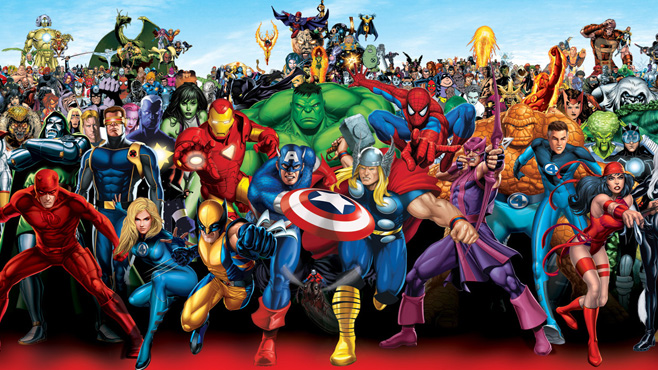
\includegraphics[width=0.85\textwidth]{images/les5-heroes.jpg}
  \caption{The superheroes being researched are only a sample from the population of all superheroes.}
  \label{fig:populatieHelden}
\end{figure}

\section{Population and sample}
\label{sec:population-and-sample}

\begin{definition}[Population]
  The set of \emph{all} items that are being researched is called the \emph{population}\index{population}.
\end{definition}

\begin{definition}[Sample]
  A subset from the population that is being researched more closely is called a \emph{sample}\index{sample}.
\end{definition}

\begin{definition}[Sampling frame]
  The \emph{sampling frame}\index{sampling frame} is a list of all members of the population.
\end{definition}

There are several reasons for using sampling:

\begin{itemize}
  \item The population is too large to do a complete census;
  \item Taking measurements is too expensive;
  \item When timing is an issue, a census may take too long;
  \item It's easier\dots
\end{itemize}

The sampling process consists of several stages:

\begin{enumerate}
  \item \textbf{Defining the population}: Who is part of the population? This is closely related to the problem statement. It's an important step that should not be taken lightly. Elements of note include a.o.~social, demographic or physical properties like gender, age, place of residence, etc.
  
  \item Specifying the \textbf{sampling frame}: Generating a list of the members of the population. For a political opinion poll, this may be an electoral register.
  
  \item Choosing a suitable \textbf{sampling method} and sample size: See Section~\ref{sec:choosing-a-sampling-method}.
\end{enumerate}

\section{Choosing a sampling method}
\label{sec:choosing-a-sampling-method}

\begin{definition}
  A \emph{random sample}\index{sample!random} (also: probability sample\index{sample!probability}) is a selection from the population where each individual has an equal probability of being selected.
\end{definition}

An important result in statistics is that under the assumption that a sample is truly random and the sample is sufficiently large, results for that sample will hold for the entire population.

A \emph{non-probability sample}\index{sample!non-probability} does \emph{not} have this property. Consequently, results within the sample \emph{cannot} be generalised.

\subsection{Stratified sampling}

Often, the population that is being studied is very heterogeneous and differs in important properties (e.g. demographics). In this case, the population may be partitioned into non-overlapping and homogenous classes or \emph{strata}. Examples are a.o.~gender, age categories, income range, or educational level.

\begin{definition}[Stratified Sample]
A \emph{stratified}\index{sample!stratified} sample is proportional when the share of the subpopulation in the sample is proportional to the share in the entire population.
\end{definition}

\begin{example}
  Table~\ref{tab:heldenPopulatie1} gives the frequencies of age and gender in the population of superheroes. Since a census among the superheroes is infeasible, we decide to take a stratified sample. Table~\ref{tab:heldenPopulatie2} gives an example where the size of each stratum is proportional to the group's size in the population.
\end{example}

  \begin{table}
  \centering
    \begin{tabular}{l|cccc|c}
      & \multicolumn{4}{c|}{\textbf{Age}} & \\
      Gender & $\le 18$ & $]18,25]$ & $]25, 40]$ & $> 40$ & Total\\
      \hline
      Female & 500 & 1500 & 1000 & 250 & 3250 \\
      Male   & 400 & 1200 & 800 & 160 & 2560\\
      \hline
      Total  & 900 & 2700 & 1800 & 410 & 5810
    \end{tabular}
    \caption{Frequencies of the superheroes in the population according to gender and age categories.}
    \label{tab:heldenPopulatie1}
\end{table}

\begin{table}
  \centering
    \begin{tabular}{l|cccc|c}
      & \multicolumn{4}{c|}{\textbf{Age}} & \\
      Gender & $\le 18$ & $]18,25]$ & $]25, 40]$ & $> 40$ & Total\\
      \hline
      Female & 50 & 150 & 100 & 25 & 325 \\
      Male   & 40 & 120 & 80 & 16 & 256\\
      \hline
      Total & 90 & 270 & 180 & 41 & 581
    \end{tabular}
      \caption{Stratified sample of the superhero population.}
    \label{tab:heldenPopulatie2}
  \end{table}


\subsection{Sample errors}
\label{ssec:sample-errors}

\paragraph{Random sampling errors}

Random variations in the sampling due to random selection

\paragraph{Systematic sampling errors}

Or selection bias. An example could be an online survey: members of the population without an internet connection cannot participate, so the sample will not be completely random.

\paragraph{Random non-sampling errors}

This includes a.o.~wrong answers or differences in interpretation of the questions.

\paragraph{Systematic non-sampling errors}

Members of the population that have a positive affinity with the research subject (or with science and research in general) are more inclined to participate and will respond with more positive answers. These will not be representative for the entire population.

\subsection{Sample standard deviation}
\label{ssec:sample-standard-deviation}

While the mean over the entire population is notated $\mu$, the \emph{sample mean}\index{mean!sample} is notated as $\overline{x}$ (see also Definition~\ref{def:mean}). Likewise, the sample standard deviation\index{standard deviation!sample} is notated $s$ instead of $\sigma$ (= the population standard deviation).

For the calculation of the sample variance\index{variance!sample}, the formula from Equation~\ref{eq:variance} is adapted:

\begin{equation}
  \label{eq:sample-variance}
  s^2 = \frac{1}{n-1} \sum_{i=1}^{n} (\overline{x} - x_i)^{2}
\end{equation}

Specifically, the denominator of the fraction is $(n-1)$ instead of $n$ (the sample size). 

Since the sum of differences $x_{i} - \overline{x}$ will always be 0 (see Equation~\ref{eq:sumGemid}), and the last difference can be calculated from the first $n-1$ differences. That is, we're not calculating the average deviations of $n$ independent numbers. Only $n-1$ of the squared differences can ``vary freely''. The number $n-1$ is also called the \emph{degrees of freedom}\index{degrees of freedom} of the variance or standard deviation.

\begin{equation}
 \sum_{i}^{n}(x_{i} - \overline{x}) = \sum_{i}^{n}x_{i} - \sum_{i}^{n}\overline{x} = \sum_{i}^{n}x_{i} - n (\frac{1}{n}\sum_{i}^{n} x_{i})
\label{eq:sumGemid}
\end{equation}

\section{Probability distribution of a sample}
\label{sec:sample-probability-distribution}

\subsection{Stochastisc experiment}

A random (or stochastic) experiment needs the following elements:

\begin{definition}[Universe or Sample space] The \emph{sample space}\index{sample!space} of an experiment is the set of all possible outcomes of the experiment and is notated as $\Omega$.
\end{definition}

\textbf{Remarks}
\begin{itemize}
\item The sample space should be \emph{complete}. Every possible outcome should be an element of $\Omega$.
\item Additionally, every outcome of an experiment should correspond with \emph{exactly one} element of $\Omega$.
\item After executing an experiment, it is possible to unambiguously determine which element of $\Omega$ has occurred.
\end{itemize}

\begin{definition}[Event]
  An \emph{event}\index{event} is a subset of the sample space. A singular or elementary event is a singleton. A composite event has a cardinality greater than 1.
\end{definition}

Events that don't have common outcomes are called \emph{disjoint}\index{event!disjoint}. Consequently, disjoint events can never occur simultaneously. When events $A$ and $B$ are disjoint, then $A \cap B = \emptyset$. When $A$ and $B$ are events, the following events can be formed:

 \begin{itemize}
  \item $A$ \textbf{or} $B$, notated $A \cup B$;
  \item $A$ \textbf{and} $B$, notated $A \cap B$;
  \item \textbf{not} $A$, notated $\overline{A}$.
\end{itemize}

\textbf{Remarks}
\begin{itemize}
\item It can be proven by induction that the union of $n$ events $A_1$ up to $A_n$ is also an event.
\item The same goes for the intersection between events.
\item For some application, countably infinite unions or intersections are considered.
\end{itemize}

\begin{definition}[Probability space] The probability of an event $A$ is notated $P(A)$. Probabilities of events should meet the following requirements:
  
\begin{enumerate}
  \item Probabilities of events are nonnegative: $\forall A \subset \Omega: P(A) \geq 0$
  \item The total of all probabilities over $\Omega$ is 1: $P(\Omega) = 1.$
  \item If $A$ and $B$ are \emph{disjoint} events, then:
    \[P(A\cup B) = P(A) + P(B). \]
\end{enumerate}

When the probability function $P$ meets these requirements (axioms), then the triple $(\Omega, \mathcal{P}(\Omega), P)$ is a \emph{probability space}\index{probability space} (with $\mathcal{P}(\Omega)$ the \emph{power set} of $\Omega$, i.e.~the set of all its subsets).
\end{definition}

\begin{example}
  \label{ex:die}
  Consider a sample space $\Omega =  \left\{ 1,2,3,4,5,6 \right\} $ and a probability function $P(\omega) = \frac{1}{|\Omega|}$, then this could represent a die with 6 sides, and outcomes $1, \ldots, 6$, each with probabilities $P(\omega) = \frac{1}{6}$.
\end{example}

\subsection{Probability distribution}
\label{ssec:probability-distribution}

\paragraph{Discrete probability distribution}

If we continue with the example of throwing a die (see Example~\ref{ex:die}), then the probability of each outcome $\Omega = \{1,2,3,4,5,6\}$ can be summarised in a table or histogram (see Figure~\ref{fig:probabilities-1-die}). Remark that:

\begin{enumerate}
  \item All probabilities are nonnegative.
  \item The probability of a specific outcome equals the area of the corresponding bar.
  \item The total area of all bars is 1.
\end{enumerate}

\begin{figure}
  \centering
  \begin{tikzpicture}
  \begin{axis}[ybar,ytick=data, anchor=north, bar width=1, yscale=.5]
  \addplot[fill=HoGentBlue]
  coordinates {
    (1, 1/6)
    (2, 1/6)
    (3, 1/6)
    (4, 1/6)
    (5, 1/6)
    (6, 1/6)};
  \end{axis}
  \end{tikzpicture}
  \caption{Probabilities for throwing a single die.}
  \label{fig:probabilities-1-die}
\end{figure}

When throwing \emph{two} dice, there are $6 \times 6 = 36$ possible outcomes, some of which are equivalent. E.g. $5$ and $2$, $2$ and $5$, $3$ and $4$, etc. each total $7$. There are two possibilities to throw $3$. Consequently, $P(X=3) = \frac{2}{36}$. For $n = 1, \ldots, 7$, it holds that $P(X=n) = \frac{n-1}{36}$. Figure~\ref{fig:probabilities-2-dice} shows the corresponding histogram of probabilitites.

\begin{figure}
  \centering
  \begin{tikzpicture}
  \begin{axis}[ybar,ytick=data, anchor=north, bar width=1, yscale=.5]
  \addplot[fill=HoGentBlue]
  coordinates {
    (2, 1/36)
    (3, 2/36)
    (4, 3/36)
    (5, 4/36)
    (6, 5/36)
    (7, 6/36)
    (8, 5/36)
    (9, 4/36)
    (10, 3/36)
    (11, 2/36)
    (12, 1/36)
  };
  
  \end{axis}
  \end{tikzpicture}
  \caption{Probabilities for throwing two dice.}
  \label{fig:probabilities-2-dice}
\end{figure}

It's now possible to calculate with these values:

\begin{itemize}
  \item The probability of throwing 10 or higher is the sum of the area of bars 10, 11, and 12.
  \item The probability of throwing a number between 2 and 7 (not included) is the sum of the area of bars 3, \ldots, 6.
  \item etc.
  \item The total area is 1: the probability that 1 of all these outcomes occurs is of course 100\%.
\end{itemize}

\subsubsection{Continuous probability distribution}

Continuous probability distributions\index{probability distribution!continuous} are distributions where the sample space doesn't merely consist of a limited number of outcomes (nominal or ordinal level of measurement), but where outcomes can be any numeric value (interval and ratio level).

Take for example the weight of our superheroes: this is a continuous variable since a value can be not only a whole number like $70$ kg or $95$ kg, but also (approximately) $86,8735485653$ kg. In principle, any real value is possible, although in practice it's impossible to measure this exactly. This has an important consequence for the probability distribution. This wil now no longer consist of separate bars, but has become a continuous curve (see Figure~\ref{fig:verdelingReactievermogen}). That means that the probability of measuring exactly $70$ kg is effectively zero. However, when we say $70$ kg, we usually mean any value between $69.5$ and $70.5$ kg, or more precisely the interval $[69.5, 70.5[$. Likewise, $70,00000$ kg means within the interval $[69.999995, 70.000005[$ kg.

The properties of probability distributions mentioned above still hold. The surface below the curve totals to 1. Also, the probability between two values is the surface below the curve, between the boundaries defined by these values. Remark that it's not actually important whether the limits are included or not, since their probabilities are negligable.

\section{The normal distribution}
\label{sec:normal-distribution}

\begin{figure}
\centering
\begin{tikzpicture}
\begin{axis}[
  domain=0:10, samples=100,
  axis lines*=left, xlabel=$x$, ylabel=$y$,
  every axis y label/.style={at=(current axis.above origin),anchor=south},
  every axis x label/.style={at=(current axis.right of origin),anchor=west},
  height=5cm, width=12cm,
  xtick={5,3.5,6.5}, ytick=\empty,
  enlargelimits=false, clip=false, axis on top,
  grid = major
  ]
  \addplot [fill=HoGentBlue!20, draw=none, domain=0:9] {gauss(5,1.5)} \closedcycle;
  \draw [yshift=-0.6cm, latex-latex](axis cs:3.5,0) -- node [fill=white] {$\sigma$} (axis cs:6.5,0);
\end{axis}
\end{tikzpicture}
\caption{The probability of Superman's reaction speed. This curve illustrates the normal distribution with mean $\mu = 5$ ms and standard deviation $\sigma = 1.5 ms.$}
\label{fig:verdelingReactievermogen}
\end{figure}

Figure \ref{fig:verdelingReactievermogen} shows the probability distribution of Superman's reaction speed, variable $X$. The curve follows the normal distribution\index{distribution!normal} with mean 5 ms and standard deviation 1.5 ms. This is notated:
\[ X  \sim Nor(\mu = 5; \sigma = 1.5) \]

The equation of this function, the probability density, is sometimes referred to as the Gaussian bell curve, after mathematician Carl Friedrich Gauss.

\begin{equation}
  f(x|\mu, \sigma^2) = \frac{1}{\sigma \sqrt{2\pi}} e^{-\frac{1}{2} \frac{(x - \mu)^{2}}{\sigma^{2}}}
  \label{eq:normalFunction}
\end{equation}

De normal distribution has the following properties:

\begin{itemize}
  \item The probability density is bell-shaped;
  \item The probability density is symmetric around $\mu$;
  \item Because of this symmetry, mean, median and mode are equal;
  \item The total area below the bell curve and above the $x$-axis is 1;
  \item The area between $\mu - \sigma$ en $\mu + \sigma$ (the so-called sigma area) contains approximately 68\% of the observations.
  \item The area between $\mu - 2 \sigma$ and $\mu + 2 \sigma$ contains about 95\% of all observations.
  \item The area between $\mu - 3 \sigma$ and $\mu + 3 \sigma$ contains about 99.7\% of all observations.
\end{itemize}

\subsection{The standard normal distribution}
\label{ssec:standard-normal-distribution}

If the distribution of stochastic variable $X$ is $X \sim N(\mu, \sigma)$, then the distribution of $Z = \frac{X - \mu}{\sigma}$ is $Z \sim N(0,1)$. This is called the standard normal distribution\index{distribution!standard normal}.

  % Bron: http://johncanning.net/wp/?p=1202
  \begin{center}
  \begin{figure}
  \centering
    \begin{tikzpicture}
      \begin{axis}[
          no markers, domain=0:10, samples=100,
          axis lines*=left,height=6cm, width=10cm,
          xtick={-3, -2, -1, 0, 1, 2, 3}, ytick=\empty,
          enlargelimits=false, clip=false, axis on top,
          grid = major
        ]
        \addplot [smooth,fill=cyan!20, draw=none, domain=-3:3] {gauss(0,1)} \closedcycle;
        \addplot [smooth,fill=orange!20, draw=none, domain=-3:-2] {gauss(0,1)} \closedcycle;
        \addplot [smooth,fill=orange!20, draw=none, domain=2:3] {gauss(0,1)} \closedcycle;
        \addplot [smooth,fill=blue!20, draw=none, domain=-2:-1] {gauss(0,1)} \closedcycle;
        \addplot [smooth,fill=blue!20, draw=none, domain=1:2] {gauss(0,1)} \closedcycle;
        \addplot[<->] coordinates {(-1,0.4) (1,0.4)};
        \addplot[<->] coordinates {(-2,0.3) (2,0.3)};
        \addplot[<->] coordinates {(-3,0.2) (3,0.2)};
        \node[coordinate, pin={68.2\%}] at (axis cs: 0, 0.35){};
        \node[coordinate, pin={95\%}] at (axis cs: 0, 0.25){};
        \node[coordinate, pin={99.7\%}] at (axis cs: 0, 0.15){};
        \node[coordinate, pin={34.1\%}] at (axis cs: -0.5, 0){};
        \node[coordinate, pin={34.1\%}] at (axis cs: 0.5, 0){};
        \node[coordinate, pin={13.6\%}] at (axis cs: 1.5, 0){};
        \node[coordinate, pin={13.6\%}] at (axis cs: -1.5, 0){};
        \node[coordinate, pin={2.1\%}] at (axis cs: 2.5, 0){};
        \node[coordinate, pin={2.1\%}] at (axis cs: -2.5, 0){};
      \end{axis}
    \end{tikzpicture}
    \caption{The standard normal distribution with different ``zones'' indicating the percentage of observations within each zone.}
    \label{fig:standard-normal-distribution}
    \end{figure}
  \end{center}

Often, it is useful to compare observations from different normal distributions. We can \emph{normalise} an observation by calculating the distance from the mean in terms of the standard deviation. This is called the $z$-score and is calculated with:

\begin{equation}
  z = \frac{x-\mu}{\sigma}
  \label{eq:zscore}
\end{equation}

This score indicates how extreme an observation is, or how many standard deviations away from the mean it is located. These $z$-scores are so important and often used that tables were composed with the probabilities that an observation drawn from $Z$ is smaller than $z$, the so-called left tail probability\footnote{Similar tables with the right tail probability exist as well}: $P(Z<z)$.

In order to calculate probabilities for any normal distribution, the following method can be used:

\begin{enumerate}
  \item Determine the stochastic variable with the associated normal distribution ($\mu$ and $\sigma$);
  \item Calculate the $z$-for a given $x$-value;
  \item Reduce any needed probability to a left tail probability, using the probabilities of the normal distribution:
  \begin{itemize}
    \item $P(Z > z) = P(Z < -z)$ (symmetry rule);
    \item $P(Z > z) = 1 - P(Z < z)$ (100\% probability rule)
  \end{itemize}
\end{enumerate}

Plotting or sketching the needed probability is also very useful to gain insight in the calculation.

\begin{example}
What is the probability that Superman reacts in less than 4 ms?
\[ P(X < 4) = P(Z < \frac{4 - 5}{1.5} = -0.67) = 0.2514 \]
\end{example}

\begin{example}
What is the probability that he reacts in less than 7 ms?
\[ P(X < 7) = P(Z < 1.33) = 0.9082 \]
\end{example}

\begin{example}
What is the probability that he reacts in less than 3 ms?
\[ P(X<3) = P(Z < -1.33) = 0.0918 \]
\end{example}

\begin{example}
What is the probability that he reacts between 2 en 6.5 ms?
\[ P( 2 < X < 6.5) = P(X < 6.5) - P(X < 2) = P(Z < 1) - P(Z < -2) = 0,8186 \]
\end{example}

\subsection{Testing for normality}
\label{ssec:testing-for-normality}

Because of the desirable properties of the normal distribution, it's often good to know whether a sample is actually drawn from a normal distribution. Several methods exist to test for normality:

\begin{itemize}
  \item Plot a histogram for the data and look at the shape of the chart. If the observations are drawn from a normal distribution, the shape will approximate a bell curve.
  
  \item Calculate the intervals $\overline{x} \pm s$, $\overline{x} \pm 2s$, $\overline{x} \pm 3s$ and determine the percentage of observations between each interval. If the observations are normally distributed, these percentages will be about 68\%, 95\%, and 99,7\%, respectively.
  
  \item Draw a Q-Q plot\index{Q-Q plot} (normality plot, see Definition~\ref{def:qq-plot}) for the observations. If they are normally distributed, the observations will be plotted approximately on a straight line.
  
  \item Calculate the \emph{kurtosis}\index{kurtosis}, a metric for the ``sharpness'' of the distribution's ``peak'':
  
    \begin{itemize}
      \item A normal distribution has a kurtosis of 3, or, alternatively, an \emph{excess kurtosis}\index{kurtosis!excess} of 0;
      \item A ``flat'' distribution has a negative excess kurtosis;
      \item A distribution with a sharp peak has a positive excess kurtosis.
    \end{itemize}
  
  \item Calculate the \emph{skewness}\index{skewness}, a metric for the symmetry of the data:
  
    \begin{itemize}
      \item A symmetric distribution (including the normal distribution) has skewness 0;
      \item A distribution with a long left tail has a negative skewness;
      \item A distribution with a right left tail has a positive skewness;
      \item Rule of thumb: if the absolute value of the skewness exceeds $1$, the distribution is not considerd to be symmetrical.
    \end{itemize}
\end{itemize}

\begin{definition}[Q-Q plot or normality plot]
  \label{def:qq-plot}
  A normality plot, or \emph{Q-Q plot}\index{Q-Q plot}\footnote{Q stands for quantile} for a set of observations is a probability plot with the sorted observations on one axis and the associated expected $z$-values on the other axis. See Figure~\ref{fig:qqplot} for some examples. If the data is normally distributed, the observations will be plotted on or near the line $y = x$.
\end{definition}

\begin{figure}
  
  \begin{center}
  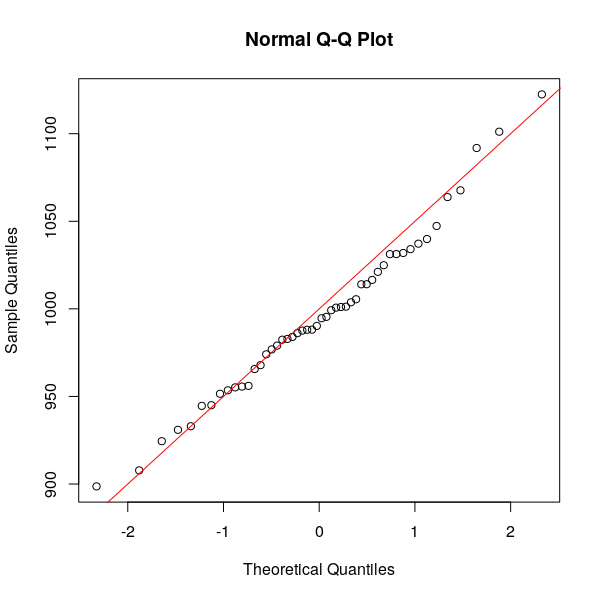
\includegraphics[width=.45\textwidth]{sampling-qqplot-good.png}
  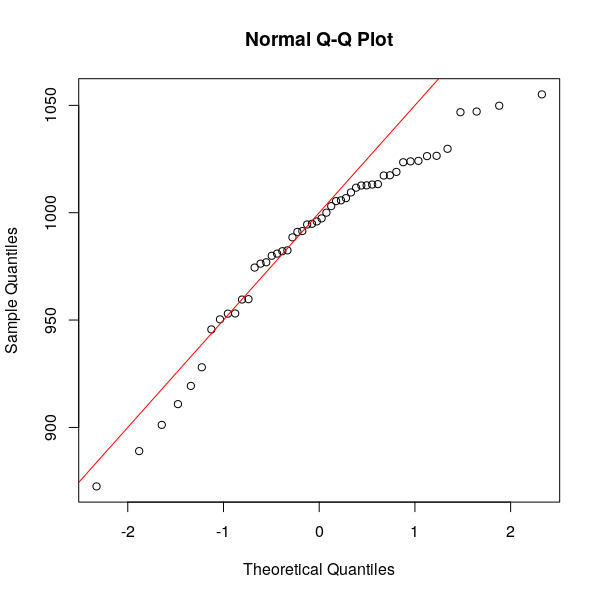
\includegraphics[width=.45\textwidth]{sampling-qqplot-bad.png}
  \end{center}
  \caption{The Q-Q plot on the left is based on a sample of 50 observations drawn from a normal distribution with mean 1000 and standard deviation of 50. The one on the right is based on a sample of 50 observations drawn from Student's $t$ distribution with 15 degrees of freedom, with the same mean and standard deviation. The lines in red are where the observations should theoretically be situated. In the plot on the left, this is more or less the case, but on the right, especially in the extremes, observations deviate from the line.}
  \label{fig:qqplot}
\end{figure}

\subsection[The chi-square distribution]{The $\chi^{2}$ verdeling}
\label{ssec:chi-square-distribution}

Let $X_{1}, X_{2}, \dots X_{v}$ be independent stochastic variables that are standard normally distributed ($\sim N(0,1)$). The $\chi^{2}$ (chi-square) variable is defined as:

\begin{equation}
  \chi^{2}_{v} = X_{1}^{2} + X_{2}^{2} + \dots + X_{v}^{2} 
\end{equation}

The number $v$ denotes the degrees of freedom\index{degrees of freedom} of the variable. $\chi^{2}$ is a continuous stochastic variable, that is always positive, since it is the sum of squares. The probability density function is:

\[ f_{n}(x) = \frac{1}{2^{\frac{n}{2}}\Gamma(\frac{n}{2})} x^{\frac{n}{2} -1} e^{\frac{x}{2}} \]

The expected value (= mean) is $v$ and variance is $2v$. The mode for $v \geq 2$ is $v-2$.

The $\chi^{2}$ variable does not occur ``in the wild.'' No natural phenomenon can be modelled with this distribution. Nevertheless, it will be quite important further on in this course.

\section{Central limit theorem}
\label{sec:central-limit-theorem}

In this section, we'll discuss one of the most fundamental results in statistics and the foundation of sampling: the central limit theorem.

\begin{theorem}
  A linear combination of a sufficiently large number of independent, identically distributed stochastic variables (i.e. with a well defined expected value and variance) will approximate the normal distribution, regardless the underlying distribution.
\end{theorem}

The proof of this theorem is outside the scope of this course, even though it is surprisingly easy to understand.

\begin{theorem}[The Central limit theorem]
  Consider a random sample of $n$ observations drawn from a population with expected value $\mu$ and standard deviation $\sigma$.
  
  If $n$ is sufficiently large, the probability distribution of the sample mean $\overline{x}$ will approximate a normal distribution with expected value $\mu_{\overline{x}} = \mu$ and standard deviation $\sigma_{\overline{x}} = \frac{\sigma}{\sqrt{n}}$.
  
  The larger the sample, the better the probability distribution of $\overline{x}$ will approximate the expected value of the population, $\mu$.
\end{theorem}

Consequently, when you draw a random sample from independent variables with some unknown distribution, the sample mean will be normally distributed. When we repeat this proces again and again (each time with the same sample size), and record the mean, we approximately obtain the graph of a normal distribution. The larger the sample size, the better the approximation.

What is particularly noteworthy is that the sample mean is normally distributed, regardless the underlying distribution!

This opens the door for a number of applications that are of capital importance to statistics. Particularly, it allows us to draw conclusions for an entire population based only on a subset: a random sample.

\subsection{Application of the central limit theorem}

When drawing a random sample of a sufficiently large size $n$ form a population with an unknown $\mu$ and (known) standard deviation $\sigma$, the probability distribution of the sample mean is a stochastic variable $M \sim N (\overline{x}, \frac{\sigma}{\sqrt{n}})$.

\begin{example}
  Let's consider the reaction time of all our superheroes and assume we have drawn a random sample $n = 100$ and $\overline{x} = 90, \sigma = 60$ (ms).
  
  We can then ask ourselves: what is the probability that the average reaction time of a superhero is below $104$ ms?

  \begin{enumerate}
    \item The stochastic variable here is the average reaction speed $\overline{x}$ in a sample of $n=100$ superheroes. Because of the central limit theory, the following holds:
    \[ \overline{x} \sim Nor(\mu = 90, \sigma_{\overline{x}} = \frac{60}{\sqrt{100}} = 6) \]
    \item We can calculate the associated $z$-score:
    \[ z = \frac{104-90}{\frac{60}{\sqrt{100}}} = \frac{104-90}{6} = 2.33 \]
    \item And therefore: $P(\overline{x} < 104) = P(Z < 2.33) = 1 - 0.0099 \approx 0.99$ or about 99\%
  \end{enumerate}
\end{example}

\subsection{Estimating stochastic parameters}
\label{ssec:estimating-stochastic-parameters}

If we want to study a sample, it is usually with the goal of drawing conclusions with regards to the population as a whole. For example, we want to know the average strength of a superhero, or the fraction of rich superheroes. 

In general, we'll \emph{estimate} a parameter of the population based on the sample. For example, $\overline{x}$ is used as an estimate of $\mu$. This type of estimation is defined as:

\begin{definition}[point estimate]
  A \emph{point estimate}\index{estimate!point} for a population parameter is a formula or equation that allows us to calculate a value to estimate that parameter.
\end{definition}

Another type of estimates are the \emph{interval estimates}\index{estimate!interval}, a.o.~confidence intervals. These are discussed in the next sections.

\subsection{Confidence interval for population mean for a large sample}
\label{ssec:confidence-interval-pop-mean-large-sample}

When we estimate the population mean from a sample, we have no idea how correct this estimate is. However, the properties of the normal distribution allow us to construct an interval that will contain the population mean with the desired level of confidence.

\begin{definition}[Confidence interval]
  A \emph{Confidence interval}\index{confidence interval} is an equation or formula that allows us to construct an interval that will contain the parameter to be estimated with a certain level of confidence.
\end{definition}

An initial estimate for the population mean is of course the sample mean:

\[ \overline{x} = \frac{1}{n} \sum_{i} x_{i} \]

Of course this estimate is not the real population mean. However, because of the central limit theorem, we know that the mean of a sample of size $n$ is normally distributed with mean $\mu$ and standard deviation $\frac{\sigma}{\sqrt{n}}$

After standardisation, we get:
\[ Z = \frac{\overline{x} - \mu}{\frac{\sigma}{\sqrt{n}}} \]
This expression depends on $\mu$, but we know that it's normally distribution. That means that we can find limits $-z$ and $z$, independent from $\mu$, that will contain $Z$ with a confidence level $1 - \alpha$ that can be chosen by the researcher. In this example, we choose $1 - \alpha= 0.95$ (and consequently $\alpha = 0.05$).
\[P(-z < Z < z) = 1 - \alpha = 0.95 \]
By applying the rule of symmetry, we find that we need to determine $z$ with:
\[ P( Z < z) = 0.975 \]
When we look this up in a Z-table, we'll find $z = 1.96$. Or, alternatively, we can calculate \verb|qnorm(0.975)| in R.

The confidence interval then is:
\[ P( -1.96 < \frac{\overline{x} - \mu}{\frac{\sigma}{\sqrt{n}}} < 1.96 ) = 1 - \alpha\]
and so
\[ P ( \overline{x} -1.96 \frac{\sigma}{\sqrt{n}} <\mu < \overline{x} + 1.96 \frac{\sigma}{\sqrt{n}}) = 1 - \alpha \]

With this technique, we can determine the bounds of an interval that will contain $\mu$ with confidence level of 95\%. If you would repeatedly draw a sample from this population and calculate the confidence interval around $\overline{x}$, then in 95\% of the cases, we expect the actual $\mu$ to be inside of the interval bounds.

Remark that we assume to know the standard deviation of the population, which is generally not the case. If the sample size is sufficiently large, the sample standard deviation is used as a point estimate for the population standard deviation.

\[ P ( \overline{x} -1,96 \frac{\sigma_{\overline{x}}}{\sqrt{n}} < \mu < \overline{x} + 1,96 \frac{\sigma_{\overline{x}}}{\sqrt{n}}) = 1 - \alpha \]


\begin{figure}
\centering
\begin{tikzpicture}
\begin{axis}[
  domain=-3:3, samples=100,
  axis lines*=left, xlabel=$z$,
  every axis y label/.style={at=(current axis.above origin),anchor=south},
  every axis x label/.style={at=(current axis.right of origin),anchor=west},
  height=5cm, width=12cm,
  xtick={-1.96,0,1.96}, ytick=\empty,
  enlargelimits=false, clip=false, axis on top,
  grid = major
  ]
  \addplot [fill=cyan!20, draw=none, domain=-3:3] {gauss(0,1)} \closedcycle;
  \draw [yshift=-0.6cm, latex-latex](axis cs:-1.96,0) -- node [fill=white] {$\sigma$} (axis cs:1.96,0);
\end{axis}
\end{tikzpicture}
\caption{Standaardnormale verdeling die 95\% betrouwbaarheidsinterval aanduidt.}
\label{fig:verdelingStandaardnormaal}
\end{figure}

\subsection{Confidence interval for population mean for a small sample}
\label{ssec:confidence-interval-pop-mean-small-sample}

In the case of small samples, we can no longer assume that the probability distribution of $\overline{x}$ approximates the normal distribution. The central limit theorem only holds for sample sizes of about $n > 30$.

The shape of the probability distribution of $\overline{x}$ now depends of the shape of the underlying probability distribution of the population. Even thoug $\sigma_{\overline{x}} = \frac{\sigma}{\sqrt{n}}$ still holds, the sample standard deviation $s$ may be a bad estimate for $\sigma$ if the sample is small.

However, there is a solution in the form of the so-called Student's $t$ distribution. Instead of:
\[ z = \frac{\overline{x} - \mu}{\frac{\sigma}{\sqrt{n}}} \]
we use the $t$-score:
\[ t = \frac{\overline{x} - \mu}{\frac{s}{\sqrt{n}}} \]

The probability density of Student's $t$ distribution is very similar to the standard normal distribution: bell-shaped, symmetrical, and with an expected value of 0.

The exact shape depends on the sample size $n$, or more precisely on the degrees of freedom\index{degrees of freedom} $(n-1)$ (abbreviated to $df$).

Remark that:
\begin{itemize}
  \item $(n-1)$ was also used to calculate the sample variance $s^{2}$;
  \item When $n \rightarrow \infty$ this converges to the standard normal distribution.
\end{itemize}

In order to calculate a confidence interval for a sample with a small number of observations, we need to do the determine:
\[ \overline{x} \pm t_{\frac{\alpha}{2}}\left(\frac{s}{\sqrt{n}}\right) \]
with $t_{\frac{\alpha}{2}}$ based on $(n-1)$ degrees of freedom. We still assume that the sample is random and drawn from a population that is approximately normally distributed.

\subsection{Confidence interval for population fraction for a large sample}
\label{ssec:confidence-interval-pop-fraction-large-sample}

If you want to measure a variable as a fraction, for example the percentage of people that responded with ``yes'' to a specific question, this is equivalent to estimating the probability $p$ on success in a binomial experiment, i.e.~an experiment with a sample space consisting of two elements, ``success'' and ``failure''. If the probility of ``success'' is $p$, the probability of ``failure'' is $q = 1 - p$. The value of $p$ can be estimated from the sample:

\[ \overline{p} = \frac{\textnormal{number of successes}}{n} \]

In order to calculate a confidence interval for $\overline{p}$, we need to know the probability distribution of $\overline{p}$. The central limit theory can then be applied to the average number of successes in a sample of size $n$. The probability distribution of $\overline{p}$ has the following properties:

\begin{itemize}
  \item Expected value of the probability distribution of  $\overline{p}$ is $p$.
  \item The standard deviation of the probability distribution of $\overline{p}$ is $\sqrt{\frac{pq}{n}}$
  \item For large samples, $\overline{p}$ is approximately normally distributed.
\end{itemize}

Since $\overline{p}$ is the sample mean of the number of successes, this allows us to calculate a confidence interval, analougous to the one for $\overline{x}$ for large samples.

\begin{definition}[Confidence interval for $p$ for a large sample]
  \[ \overline{p} \pm z_{\frac{\alpha}{2}} \sqrt{\frac{\overline{p}\overline{q}}{n}} \]
  with $\overline{p} = \frac{x}{n}$ and $\overline{q} = 1- \overline{p}$
\end{definition}


%\chapter{Hypothesis tests}
\label{ch:hypothesis-tests}

%In de voorbije hoofdstukken hebben we gezien hoe we aan de hand van steekproefonderzoek bepaalde kerngetallen over een populatie kunnen berekenen, bijvoorbeeld aan de hand van puntschatters of betrouwbaarheidsintervallen. We kunnen deze informatie ook gebruiken om bepaalde hypothesen over een populatie te toetsen. Een hypothese is een veronderstelling waarvan nog bewezen moet worden dat ze correct is. Het doel van een toetsingsprocedure is het testen van een hypothese omtrent de waarden van 1 of meerdere populatieparameters.
%
%\begin{definition}[Statistische hypothese.]
%  Een statische hypothese\index{hypothese!statistische} is een uitspraak over de numerieke waarde van een populatieparameter.
%\end{definition}
%
%Voorbeelden van hypothesen:
%
%\begin{itemize}
%  \item Gemiddeld redt een superheld minstens 3,3 mensen per dag.
%  \item De gemiddelde lengte van een superheld is minstens 120 cm.
%  \item \dots
%\end{itemize}
%
%In dit hoofdstuk gaan we de algemene theorie over toetsen formuleren aan de hand van het testen van hypothesen over het populatiegemiddelde $\mu$, de $z$-toets. Naast de $z$-toets bestaan er echter nog vele andere statistische hypothesetoetsen die in specifieke situaties gebruikt kunnen worden. De meest geschikte statistische toets hang o.a.~af van de populatiegrootheid in kwestie (gemiddelde, standaardafwijking, enz.), en veronderstellingen over de onderliggende stochastische verdeling van de populatie (normaal verdeeld of niet, enz,).
%
%\section{Elementen van een hypothesetoets}
%\label{sec:elementen-hypothesetoets}
%
%Algemeen gezien bestaat een toetsingsprocedure uit 4 elementen:
%\begin{enumerate}
%  \item \textbf{Nulhypothese}\index{nulhypothese}\index{hypothese!nul-} $H_{0}$: Deze hypothese proberen we te ontkrachten door een redenering in het ongerijmde. We gaan deze hypothese accepteren, tenzij de observaties uit de steekproef overtuigend wijzen op het tegendeel.
%  \item \textbf{Alternatieve hypothese}\index{hypothese!alternatieve} $H_{1}$: Dit is meestal de hypothese die de onderzoeker wil bewijzen. Deze hypothese zal echter alleen worden geaccepteerd als de observaties uit de steekproef overtuigend wijzen op de juistheid ervan.
%  \item \textbf{Teststatistiek}: De veranderlijke die berekend wordt uit de steekproef
%  \item Aanvaardings- en kritiek gebied:
%  \begin{itemize}
%    \item  \textbf{Aanvaardingsgebied\index{aanvaardingsgebied}\index{gebied!aanvaardings-}}: Het gebied van waarden die de nulhypothese $H_{0}$ ondersteunt
%    \item \textbf{Verwerpingsgbied\index{verwerpingsgebied}\index{gebied!verwerpings-}}: gebied dat waarden bevat die de nulhypothese verwerpen. Ook kritiek gebied\index{gebied!kritiek} genoemd.
%  \end{itemize}
%\end{enumerate}
%
%Een alternatief voor de laatste stap is het berekenen van de \emph{overschrijdingskans} (zie verder).
%
%De beslissing om de nulhypothese $H_{0}$ te verwerpen of te aanvaarden is gebaseerd op informatie uit een steekproef, getrokken uit de populatie waarover de hypothese is geformuleerd. De steekproefwaarden worden gebruikt om 1 enkele waarde van een teststatistiek te berekenen die de beslissing zal bepalen. Daartoe worden alle waarden die de teststatistiek kan aannemen, verdeeld in twee gebieden, \begin{inparaenum}[(i)] \item het aanvaardingsgebied en \item het verwerpingsgebied\end{inparaenum}. Indien de waarde van de teststatistiek ligt in het verwerpingsgebied, dan wordt de nulhypothese verworpen en de alternatieve hypothese aanvaard. Indien de waarde van de teststatistiek in het aanvaardingsgebied valt dan wordt de nulhypothese aanvaard.
%
%\section{Toetsingsprocedure voor de \texorpdfstring{$z$}{z}-toets}
%\label{sec:toetsingsprocedure-z-toets}
%
%In de eerste toetsingsprocedure die we in deze cursus uitwerken, gaan we een uitspraak over het populatiegemiddelde $\mu$ verifiëren. Deze is algemeen bekend als de $z$-toets\index{$z$-toets}\index{toets!$z$-}.
%
%\begin{enumerate}
%  \item De vermoedens over de populatie worden vastgelegd in twee hypothesen $H_{0}$ en $H_{1}$. Voor de (rechtszijdige) $z$-toets is de nulhypothese dat het populatiegemiddelde $\mu$ een bepaalde waarde heeft, en de alternatieve hypotehese dat $\mu$ \emph{groter} is.
%  \item Het significantieniveau\index{significantieniveau}\index{niveau!significantie-} $\alpha$ en steekproefomvang $n$ worden vastelegd. Je kan $\alpha$ in principe zelf kiezen (bv. 0,05)\footnote{Merk op dat het significantieniveau gerelateerd is aan het betrouwbaarheidsniveau $1-\alpha$. Zie Sectie~\ref{ssec:betrouwbaarheidsinterval-grote-steekproef}}. Hoe dichter het significantieniveau bij 0 ligt, hoe minder twijfel er is over het resultaat van de toets. Maar langs de andere kant wordt het ook moeilijker om de nulhypothese te verwerpen.
%  \item De waarde van de toetsingsgrootheid in de steekproef wordt berekend. De uitkomst is bepalend voor de beslissing of we de nulhypothese $H_{0}$ kunnen verwerpen of niet. We weten dankzij de centrale limietstelling dat de kansverdeling van het steekproefgemiddelde $M \sim Nor( \mu, \frac{\sigma}{\sqrt{n}})$.
%  \item Het kritieke gebied bepalen, of meer bepaald de grens tussen het aanvaardings- en het verwerpingsgebied. We zoeken een grenswaarde\index{kritieke grenswaarde} $g$ zodat:
%  
%  \begin{equation}
%  \begin{split}
%  P(M > g) = \alpha & \Leftrightarrow P\left(Z> z=\frac{g-\mu}{\sigma/\sqrt{n}}\right) = \alpha & (normalisatie)\\
%  & \Leftrightarrow P\left(Z < z = \frac{g-\mu}{\sigma/\sqrt{n}}\right) = 1-\alpha & (100\%-regel)
%  \end{split}
%  \end{equation}
%  
%  De $z$-waarde hangt af van het gekozen significantieniveau en kan worden opgezocht in een $z$-tabel of berekend worden met de R-functie \texttt{qnorm(1-alpha)}. Daaruit kunnen we dan $g$ afleiden:
%  
%  \begin{equation}
%  z = \frac{g-\mu}{\sigma/\sqrt{n}} \Leftrightarrow g = \mu + z \frac{\sigma}{\sqrt{n}}
%  \label{eq:kritieke-grenswaarde-z-toets}
%  \end{equation}
%
%  Alle waarden \emph{links} van $g$ vormen het aanvaardingsgebied. Waarden rechts, die dus ver van het $H_0$ veronderstelde populatiegemiddelde liggen, zijn het verwerpingsgebied. Zie ook Sectie~\ref{sec:kritieke-gebied}.
%\end{enumerate}
%
%\begin{example}
%  \label{ex:hypothesetoets-dagelijkse-reddingen}
%  Algemeen wordt aangenomen dat superhelden stellen gemiddeld 3,3 mensen per dag redt. De onderzoekers krijgen echter gevoel dat dat niet zo is: ze hebben de indruk dat een superheld \emph{meer} dan $3,3$ mensen per dag redt.
%  
%  Ze gaan dit onderzoeken en voeren een steekproef uit bij $n = 30$ superhelden. In deze steekproef is het gemiddelde $\overline{x} = 3,483$ is. De standaardafwijking in de populatie is verondersteld gekend en is $\sigma = 0,55$.
%  
%  Kan hieruit besloten worden dat superhelden gemiddeld meer dan 3,3 mensen per dag redt?
%
%  \begin{enumerate}
%    \item We veronderstellen dat het aantal mensen dat een superheld redt normaal verdeeld  is en formuleren twee hypothesen omtrent de parameter $\mu$.
%    \begin{itemize}
%      \item $H_{0}$ = de nulhypothese (hetgeen we willen weerleggen). In dit geval \[ H_{0} : \mu = 3,3 \]
%      \item $H_{1}$ = alternatieve hypothese (vermoeden dat we willen aantonen). In dit geval \[H_{1}= \mu > 3,3 \]
%    \end{itemize}
%  
%    We veronderstellen in de redenering initieel dat de nulhypothese $H_{0}$ waar is. Indien het gemiddelde aantal mensen gered per dag $\overline{x}$ van de steekproef sterk afwijkt van de veronderstelde waarde, verwerpen we de nulhypothese $H_{0}$ en aanvaarden we de alternatieve hypothese $H_{1}$.
%    
%    Wat betekent nu ``sterk afwijken''? Zou je uit een populatie met gemiddelde van $3,3$ gemakkelijk een steekproef kunnen trekken met gemiddelde $3,483$? De centrale limietstelling (zie Sectie~\ref{sec:centrale-limietstelling}) laat ons toe de kans hiertoe te berekenen.
%    
%    \item Vastleggen significantieniveau $\alpha$ en steekproefomvang $n$. We willen een significantieniveau van 5\% kiezen, dus $\alpha = 0,05$. De steekproefomgang is gegeven en is hier $n = 30$.
%    
%    \item De waarde van de toetsingsgrootheid in de steekproef bepalen. We nemen hier het steekproefgemiddelde: $\overline{x} = 3,483$
%    
%    We veronderstellen in de redenering dat de nulhypothese $H_{0}$ waar is en dat we $\sigma$ goed kunnen schatten hebben ($\sigma = 0,55$). Dan geldt voor het steekproefgemiddelde $M$ volgens de centrale limietstelling dat:
%    
%    \[M \sim  Nor(\mu = 3,3; \sigma = \frac{0,55}{\sqrt{30}})\]
%    
%    De waarde $\overline{x} = 3,483$ bevindt zich erg rechts (zie Figuur~\ref{fig:hypothesetoets-reddingen-per-dag}). $\overline{x}$ ligt zelfs zo ver naar rechts dat de kans (indien $H_{0}$ waar is) om dergelijke geobserveerde waarde te krijgen of groter, zeer klein is. Een dergelijke geobserveerde waarde onder de nulhypothese kan dus moeilijk verklaard worden door louter toeval. Intu\"itief voelen we dus aan dat hoe verder de geobserveerde waarde $\overline{x}$ zich bevindt in de rechtse richting, hoe meer we geneigd zijn om de nulhypothese te verwerpen. Maar wat is te ver en wat niet?
%    
%    \item De kritieke grenswaarde berekenen. De $z$-waarde voor een significantieniveau van $0,05$ is 1,645\footnote{In R kan je dit berekenen met \texttt{qnorm(1 - 0.05)}}.
%    
%    \[ g = \mu + z \times \frac{\sigma}{\sqrt{n}} = 3,3 + 1,645 \times \frac{0,5}{\sqrt{30}} \approx 3,45 \]
%    
%    Het steekproefgemiddelde $\overline{x} = 3,483$ ligt nog verder van $\mu = 3,3$ dan de grenswaarde $g = 3,45$. De kans is heel klein dat zo'n steekproef getrokken wordt uit een populatie met dit gemiddelde. Slechts in 34 steekproeven op 1000 zal een dergelijke gebeurtenis optreden. Met andere woorden, de steekproefwaarde ligt in het verwerpingsgebied. We kunnen dus $H_0$ verwerpen en besluiten met dat superhelden inderdaad \emph{meer} dan 3,3 mensen per dag redden.
%  \end{enumerate}
%
%\end{example}
%
%\begin{exercise}
%  Kunnen we in Voorbeeld~\ref{ex:hypothesetoets-dagelijkse-reddingen} zomaar veronderstellen dat het gemiddelde normaal verdeeld is? Waarom (niet)?
%\end{exercise}
%
%\begin{figure}
%  \centering
%  \begin{tikzpicture}
%    \begin{axis}[
%        domain=3:3.6, samples=100,
%        axis lines*=left, xlabel=$z$,
%        every axis y label/.style={at=(current axis.above origin),anchor=south},
%        every axis x label/.style={at=(current axis.right of origin),anchor=west},
%        height=5cm, width=12cm,
%        xtick={3.3,3.483}, ytick=\empty,
%        enlargelimits=false, clip=false, axis on top,
%        grid = major
%      ]
%      \addplot [fill=cyan!20, draw=none, domain=3:3.6] {gauss(3.3,0.101328673)} \closedcycle;
%    \end{axis}
%  \end{tikzpicture}
%  \caption{Verdeling van het aantal mensen dat gemiddeld per dag gered wordt door een superheld (Voorbeeld~\ref{ex:hypothesetoets-dagelijkse-reddingen}). De kansverdeling voor het steekproefgemiddelde is normaal verdeeld met $\mu = 3,3$ en $\sigma = 0,5$. Het steekproefgemiddelde $\overline{x} =3,483$.}
%  \label{fig:hypothesetoets-reddingen-per-dag}
%\end{figure}
%
%\section{Kritieke gebied}
%\label{sec:kritieke-gebied}
%
%De formule voor de berekening van de grenswaarde (zie Formule~\ref{eq:kritieke-grenswaarde-z-toets}) is gebaseerd op de centrale limietstelling, en meer bepaald betrouwbaarheidsintervallen.
%
%De kritieke grenswaarde vormt een betrouwbaarheidsinterval rond $\mu$ met een gekozen zekerheidsniveau. Als we bijvoorbeeld stellen dat $\alpha = 0.05$, weten we vanuit de centrale limietstelling dat we kunnen verwachten dat als we herhaaldelijk voldoende steekproeven uit deze populatie nemen, in 95\% van de gevallen het steekproefgemiddelde binnen dit betrouwbaarheidsgeval zal liggen.
%
%Als we de redenering omkeren, en een steekproef genomen hebben waar het gemiddelde $\overline{x}$ \emph{niet} binnen dit betrouwbaarheidsinterval ligt, dan is de kans heel klein (kleiner dan 5\%) dat deze uit een populatie getrokken is met het veronderstelde gemiddelde $\mu$. In dat geval kunnen we de nulhypothese dus verwerpen.
%
%In Voorbeeld~\ref{ex:hypothesetoets-dagelijkse-reddingen} is de kritieke grenswaarde het getal $g$ waarvoor geldt dat
%
%\[ P(M > g) = \alpha \]
%
%wat dan wordt verder uitgewerkt als:
%
%\[ P(Z > \frac{g - \mu}{\frac{\sigma}{\sqrt{n}}}) = \alpha \]
%
%waaruit volgt dat:
%
%\begin{equation}
%  \label{eq:kritieke-waarde-rechtszijdig}
%  g = \mu + z \times \frac{\sigma}{\sqrt{n}}
%\end{equation}
%
%\section{Overschrijdingskans}
%\label{sec:overschrijdingskans}
%
%Een karakteristiek die gebruikt wordt om weer te geven hoe sterk de geobserveerde waarde afwijkt van $H_{0}$, is de overschrijdingskans (probability value of ook $p$-waarde\index{$p$-waarde}). Dit vormt een alternatieve manier om te bepalen of de nulhypothese al dan niet verworpen kan worden.
%
%\begin{definition}[overschrijdingskans]
%  De \emph{overschrijdingskans}\index{overschrijdingskans} is de kans, indien de nulhypothese waar is, om een waarde te verkrijgen van de toetsingsgrootheid die minstens even extreem is als de geobserveerde waarde.
%\end{definition}
%
%\begin{definition}[statistische significantie]
%  In een statistische hypothesetoets heeft men een \emph{statistisch significant}\index{significant} resultaat behaald waneer de geobserveerde overschrijdingskans $p$ van de teststatistiek lager is dan het significantieniveau $\alpha$. De $p$-waarde wordt onder het gekozen significantieniveau beschouwd als te extreem om de veronderstelling dat de nulhypothese waar is aan te houden.
%\end{definition}
%
%\begin{example}
%  In het onderzoek naar het aantal dagelijkse reddingen door superhelden (Voorbeeld~\ref{ex:hypothesetoets-dagelijkse-reddingen}) kan de overschrijdingskans als volgt berekend worden:
%  
%\[ P(M > 3,483) = P \left(Z> \frac{3,483 - 3,3}{\frac{\sigma}{\sqrt{n}}}\right) = P (Z > 1,822) = 0,0344 \]
%\end{example}
%
%Als de overschrijdingskans of $p$-waarde kleiner is dan de onbetrouwbaarheidsdrempel dan moet $H_{0}$ verworpen worden, is de $p$-waarde gelijk of groter dan $\alpha$ dan mag je $H_{0}$ niet verwerpen. In ons geval is de $p$-waarde $0,0344$ en die is kleiner dan $\alpha = 0,05$ dus moeten we $H_{0}$ verwerpen.
%
%\begin{itemize}
%  \item $p$-waarde $< \alpha \Rightarrow$ $H_{0}$, verwerpen want de gevonden waarde voor $\overline{x}$ is te extreem;
%  \item $p$-waarde $\geq \alpha \Rightarrow$ $H_{0}$ niet verwerpen, want de gevonden waarde voor $\overline{x}$ kan nog verklaard worden door toeval.
%\end{itemize}
%
%\section{Eenzijdig of tweezijdig toetsen}
%\label{sec:eenzijdig-of-tweezijdig}
%
%In Voorbeeld~\ref{ex:hypothesetoets-dagelijkse-reddingen} gaat het om een hypothese waar we vermoeden dat het populatiegemiddelde \emph{hoger} ligt dan een bepaalde waarde. We twijfelen dus aan de de nulhypothese als ons steekproefgemiddelde significant boven het vooropgestelde gemiddelde $\mu = 3,3; \alpha = 0,05$ ligt. Het kritieke gebied om $H_{0}$ te verwerpen ligt dus aan de rechterzijde van de curve en we noemen deze toets dan ook rechtszijdig.
%
%We zouden ook een toets kunnen maken waar we denken dat de superhelden gemiddeld \emph{minder} mensen redden per dag. Dan ligt het kritieke gebied aan de linkerzijde en noemen we de toets linkszijdig.
%
%\begin{exercise}
%  \label{ex:critical-value-left-tail}
%  Wat zou je in vergelijking \ref{eq:kritieke-waarde-rechtszijdig} moeten veranderen opdat je de correcte kritieke waarde zou berekenen voor een linkszijdige $z$-toets?
%\end{exercise}
%
%Soms kan het ook zijn dat er tweezijdig moet getoetst worden. De alternatieve hypothese wordt dan geformuleerd als zijnde dat het populatiegemiddelde verschillend is van de opgegeven waarde. Er moeten dan twee kritieke grenswaarden berekend worden namelijk de linker- en de rechter grenswaarden.
%
%\begin{equation}
%  g = \mu \pm z \times \frac{\sigma}{\sqrt{n}}
%  \label{eq:kritieke-waarde-tweezijdig}
%\end{equation}
%
%De totale oppervlakte van het kritieke gebied moet $1 - \alpha$ zijn, en je moet er rekening mee houden dat zowel links als rechts een gebied met telkens oppervlakte $\alpha / 2$ samen het aanvaardingsgebied vormen. Je moet dan ook de overeenkomstige $z$-waarde kiezen. Als we opnieuw significantieniveau $\alpha = 0,05$ nemen, zoeken we dus de $z$ waarde waarvoor geldt dat;
%
%\[P(Z < -z) + P(Z > z) = \alpha \Leftrightarrow 2 P(Z>z) = \alpha \Leftrightarrow P(Z < z) = 1-\frac{\alpha}{2} = 0,975\]
%
%De overeenkomstige $z$-waarde is dan ongeveer 1.96 (op te zoeken in de $z$-tabel of in R met \texttt{qnorm(.975)}).
%
%De drie vormen van de $z$-toets worden samengevat in tabel~\ref{tab:toetsingsprocedures}.
%
%\begin{table}
%  \centering
%  \begin{tabular}{l|ccc}
%    \toprule
%    Doel              & \multicolumn{3}{l}{\parbox{.5\textwidth}{Test op gemiddelde waarde $\mu$ van de populatie aan de hand van een steekproef van $n$ onafhankelijke steekproefwaarden}} \\
%    \midrule
%    Voorwaarde        & \multicolumn{3}{l}{\parbox{.5\textwidth}{De populatie is willekeurig verdeeld, $n$ voldoende groot}} \\
%    \midrule
%    Type test         & Tweezijdig           & Eenzijdig links & Eenzijdig rechts \\
%    \midrule
%    $H_{0}$           & $\mu = \mu_{0}$      & $\mu = \mu_{0}$ & $\mu = \mu_{0}$  \\
%    $H_{1}$           & $\mu \neq \mu_{0}$   & $\mu < \mu_{0}$ & $\mu > \mu_{0}$  \\
%    Verwerpingsgebied & $\left|z\right| > g$ & $z< -g $        & $z>g$            \\
%    Teststatistiek    & \multicolumn{3}{c}{$z = \frac{\overline{x} - \mu_{0}}{\frac{\sigma}{\sqrt{n}}}$} \\
%    \bottomrule
%  \end{tabular}
%  \caption{Samenvatting verschillende vormen van de $z$-toets}
%  \label{tab:toetsingsprocedures}
%\end{table}
%
%\section{De \texorpdfstring{$z$}{z}-toets in R}
%\label{sec:z-toets-R}
%
%Het codevoorbeeld hieronder is de uitwerking van Voorbeeld~\ref{ex:hypothesetoets-dagelijkse-reddingen} in R.
%
%\lstinputlisting{data/z-test.R}
%
%\begin{figure}
%  \centering
%  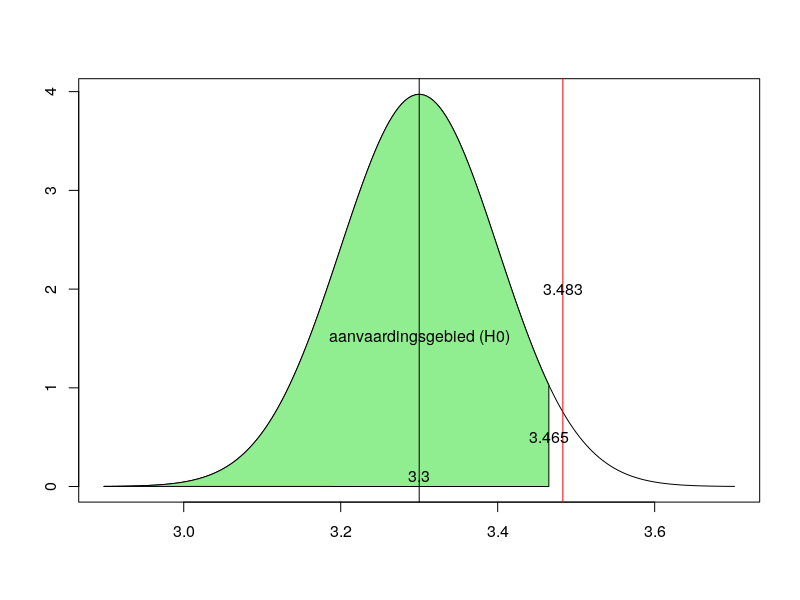
\includegraphics[width=\textwidth]{z-toets-reddingen}
%  \caption{Plot in R van de situatie van Voorbeeld~\ref{ex:hypothesetoets-dagelijkse-reddingen}}
%\end{figure}
%
%\section{Voorbeelden}
%
%\begin{example}
%  Bij een aselecte steekproef van 50 waarnemingen vinden we we volgende grootheden:
%  \begin{itemize}
%    \item $\overline{x} = 25$
%    \item $s = \sqrt{55} = 7,41$
%  \end{itemize}
%  
%  We willen weten of er reden is om aan te nemen dat $\mu$ van de populatie kleiner is dan 27.
%  
%  \begin{enumerate}
%    \item Bepalen van de hypothesen: 
%    
%    $H_{0} : \mu = 27$ en $H_{1}: \mu < 27$.
%    
%    \item Vastleggen significantieniveau $\alpha$ en steekproefomvang $n$:
%    
%    $\alpha = 0,05$ en $n=50$.
%    
%    \item Waarde toetsingsgrootheid bepalen. 
%    
%    We kiezen hiervoor het steekproefgemiddelde $M$. Volgens de centrale limietstelling geldt:
%    
%    \[ M \sim Nor(\mu = 27, \frac{\sigma}{\sqrt{n}}) \]
%    De toetsingsgrootheid is
%    \[ Z = \frac{\overline{x} - \mu}{\frac{\sigma}{\sqrt{n}}} = \frac{25-27}{\sqrt\frac{55}{50}} \approx -1,91\]
%    
%    \item Overschrijdingskans berekenen.
%    
%    We vinden een overschrijdingskans van het gemiddelde van \texttt{pnorm(-1.91)} of ongeveer $0,0281$. Bij een significantieniveau van 0,05 duidt dit er op dat we $H_{0}$ mogen verwerpen.
%    
%    \item Bereken en teken kritiek gebied.
%    
%    \[ g = \mu - z \times \frac{\sigma}{\sqrt{n}} \]
%    en dus
%    
%    \[ g = 27 - 1,645 \times \sqrt{\frac{\sigma}{n}} \]
%    \[ g =  25,27470944 \]
%    
%    We vinden dus dat $\overline{x} < g$ komen tot hetzelfde besluit, nl.~dat we $H_{0}$ kunnen verwerpen.
%    
%  \end{enumerate}
%\end{example}
%
%\begin{example}
%  In een onderzoek naar het kleingeld dat in de zakken van van onze superhelden zit, stellen de onderzoekers dat zij gemiddeld 25 euro op zak hebben. Ze gaan ervan uit de spreiding $\sigma = 7$ is. Verder zijn de gegevens van de aselecte steekproef van omvang $n=64$ beschikbaar met gemiddeld zakgeld $\overline{x}$ van 23 euro. Voor het significantieniveau kiezen ze $\alpha = 0,05$.
%  
%  \begin{enumerate}
%    \item Bepalen van de hypothesen.
%    
%    $H_{0} : \mu = 25$ en $H_{1}: \mu \neq 25$.
%    
%    \item Vastleggen significantieniveau $\alpha$ en steekproefomvang $n$.
%    
%    $\alpha = 0,05$ en $n=64$.
%    
%    \item Bepalen van de kritieke grenzen.
%    
%    \[ g_{1} = \mu - z \times \frac{\sigma}{\sqrt{n}} = 23,28 \]
%    
%    \[ g_{2} = \mu + z \times \frac{\sigma}{\sqrt{n}} = 26,72 \]
%    
%    \item Kritiek gebied.
%    
%    We vinden dat $\overline{x}$ in het kritieke gebied ligt (want $\overline{x} = 23 < g_1 = 23,25$), dus mogen we $H_{0}$ verwerpen.
%    
%  \end{enumerate}
%\end{example}
%
%\section{De \texorpdfstring{$t$}{t}-toets}
%\label{sec:t-toets}
%
%Bij de $z$-toets gaan we uit van een aantal veronderstellingen waar we rekening moeten mee houden:
%
%\begin{itemize}
%  \item De steekproef moet voldoende groot zijn ($n \ge 30$);
%  \item De variatie van de toetsingsgrootheid moet normaal verdeeld zijn;
%  \item We veronderstellen dat de standaardafwijking van de populatie, $\sigma$, gekend is.
%\end{itemize}
%
%De eerste drie voorwaarden maken dat de centrale limietstelling kan toegepast worden.
%
%Soms zijn deze veronderstellingen niet geldig en mogen we dan ook de $z$-toets \emph{niet} gebruiken! In deze gevallen kunnen we wel gebruik maken van de Student-$t$ verdeling. In de $t$-toets\index{$t$-toets}\index{toets!$t$-} wordt er wel van uit gegaan dat de onderzochte variabele normaal verdeeld is.
%
%De formule voor de kritieke grenswaarde wordt dan aangepast als:
%
%\begin{equation}
%g = \mu \pm t \times \frac{s}{\sqrt{n}}
%\label{eq:kritieke-waarde-t-toets}
%\end{equation}
%
%Voor het bepalen van de $t$-waarde hebben we het aantal vrijheidsgraden nodig, $n-1$. Om de standaardafwijking te schatten, gebruiken we de steekproefstandaardafwijking, $s$.
%
%\begin{example}
%  \label{ex:t-toets-dagelijkse-reddingen}
%  Stel dat de onderzoekers van de superhelden uit Voorbeeld~\ref{ex:hypothesetoets-dagelijkse-reddingen} door tijdsdruk niet in staat waren om een voldoende grote steekproef te nemen en slechts $n = 20$ observaties gedaan hebben, met hetzelfde steekproefgemiddelde $\overline{x} = 3,483$. De standaardafwijking in deze steekproef bleek $s = 0,55$.
%  
%  Kunnen we in deze omstandigheden, met eenzelfde significantieniveau $\alpha = 0,05$, het besluit dat superhelden dagelijks \emph{meer} dan 3,3 mensen redden aanhouden?
%  
%  \begin{enumerate}
%    \item Bepalen van de hypothesen.
%    
%      $H_{0} : \mu = 3,3$ en $H_{1}: \mu > 25$.
%    
%    \item Vastleggen significantieniveau $\alpha$ en steekproefomvang $n$.
%    
%    $\alpha = 0,05$ en $n=25$.
%    
%    \item Bepalen van de kritieke grenswaarde.
%    
%    \[ g_{2} = \mu + t \times \frac{s}{\sqrt{n}} \approx 3,3 + 1,711 \times \frac{0,55}{\sqrt{25}} \approx 3.488 \]
%    
%    De waarde voor $t$ wordt in R berekend met \texttt{qt(1-a, df = n - 1)} (met \texttt{a} het significantieniveau en \texttt{df} het aantal vrijheidsgraden.)
%    
%    \item Conclusie.
%    
%    We vinden dat $\overline{x} = 3,483$ kleiner is dan de kritieke grenswaarde en dus in het aanvaardingsgebied ligt. Met andere woorden, we mogen $H_{0}$ \emph{niet} verwerpen.
%  \end{enumerate}
%
%  Met andere woorden, ook al krijgen we gelijkaardige resultaten in onze steekproef, kunnen we niet hetzelfde besluit trekken. Omdat onze steekproef te klein is, is er grotere onzekerheid of de waarde van het steekproefgemiddelde extreem genoeg is om de nulhypothese te verwerpen.
%  
%  Hieronder vind je de uitwerking van dit voorbeeld in R.
%\end{example}
%
%\lstinputlisting{data/t-test.R}
%
%\begin{figure}
%  \centering
%  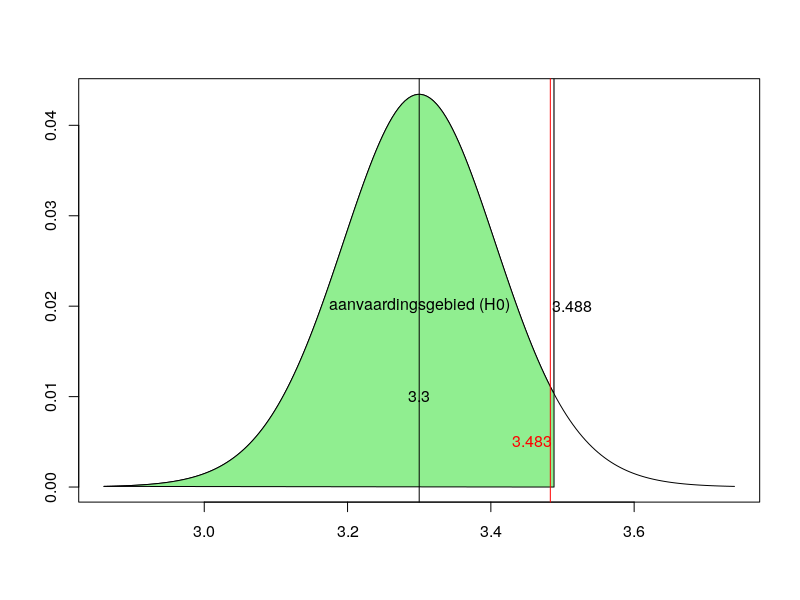
\includegraphics[width=\textwidth]{t-toets-reddingen}
%  \caption{Plot in R van de situatie van Voorbeeld~\ref{ex:t-toets-dagelijkse-reddingen}}
%\end{figure}
%
%\begin{example}
%  Een uitbraak van een door Salmonella veroorzaakte ziekte werd toegeschreven aan vanille-ijs van een bepaalde fabriek~\autocite{Lindquist}. Wetenschappers hebben het niveau van Salmonella gemeten in 9 willekeurig genomen steekproeven.
%  
%  De niveaus (in MPN/g\footnote{Most Probable Number. Zie bv.~\url{http://www.microbiologie.info/mpn-methode.html} voor meer uitleg over deze methode.}) zijn de volgende:
%  
%    \begin{center}
%    \begin{tabular}{|l|l|l|l|l|}
%      \hline
%      0,593 & 0,142 & 0,329 & 0,691 & 0,231 \\ \hline
%      0,793 & 0,519 & 0,392 & 0,418 &       \\ \hline
%    \end{tabular}
%  \end{center}
%
%  Is er reden om aan te nemen dat het Salmonella-niveau in het ijs significant groter is dan 0,3 MPN/g? We zullen gebruik maken van de R-functie \texttt{t.test} om deze vraag te beantwoorden. Lees zelf de help-pagina van deze functie om de mogelijke opties te leren kennen.
%  
%  \begin{enumerate}
%    \item Bepalen van de hypothesen
%    
%    $H_0: \mu = 0.3, H_1: \mu > 0,3$
%    
%    \item Vastleggen significantieniveau $\alpha = 0.05$ (in R moet je het betrouwbaarheidsniveau $1-\alpha$ opgeven, dus 0,95) en steekproefomvang $n = 9$
%    
%    \item Bepalen overschrijdingskans. Het gaat hier over een rechtszijdige toets, wat aangegeven wordt met de optie \texttt{alternative="greater"}. Het gekozen betrouwbaarheidsniveau is de standaardwaarde voor deze functie en moet niet expliciet meegegeven worden.
%    
%\begin{lstlisting}
%x <- c(0.593, 0.142, 0.329, 0.691, 0.231, 0.793, 0.519, 0.392, 0.418)
%t.test(x, alternative = "greater", mu = 0.3)
%\end{lstlisting}
%    
%    Het resultaat is:
%    
%\begin{verbatim}
%One Sample t-test
%
%data:  x
%t = 2.2051, df = 8, p-value = 0.02927
%alternative hypothesis: true mean is greater than 0.3
%95 percent confidence interval:
%0.3245133       Inf
%sample estimates:
%mean of x 
%0.4564444 
%\end{verbatim}
%    
%    \item Conclusie. De overschrijdingskans $p = 0,029 < \alpha = 0,05$. We kunnen dus de nulhypothese verwerpen; er is met ander worden en vrij sterke aanwijzing dat het gemiddelde Salmonella-niveau in het ijs groter is dan 0,3 MPN/g.
%    
%    Je kan uit de uitvoer van de \texttt{t.test}-functie ook het kritieke gebied aflezen: $[0,3245133; +\infty[$. Het steekproefgemiddelde $0,4564444$ ligt in het kritieke gebied, wat eveneens leidt tot de conclusie dat de nulhypothese kan verworpen worden.
%  \end{enumerate}
%\end{example}
%
%\section{De \texorpdfstring{$t$}{t}-toets voor twee steekproeven}
%\label{sec:t-toets-twee-steekproeven}
%
%De $t$-toets kan ook gebruikt worden om twee steekproeven met elkaar te vergelijken. Je kan er dan mee nagaan of het steekproefgemiddelde van beide steekproeven \emph{significant} verschillend is.
%
%Men maakt onderscheid tussen twee gevallen:
%
%\begin{itemize}
%  \item Beide steekproeven zijn onafhankelijk, zijn afzonderlijk genomen. Een voorbeeld is een onderzoek naar een medische behandelingsmethode waar een contolegroep de behandeling \emph{niet} krijgt en een testgroep de behandeling wel krijgt.
%  \item De steekproeven zijn afhankelijk, of gepaard. Een voorbeeld is twee metingen uitvoeren op hetzelfde lid van de populatie, zoals de koorts nemen voor en na het innemen van een medicijn om het effect ervan te meten.
%\end{itemize}
%
%In R kan je eveneens de functie \texttt{t.test} gebruiken voor het uitvoeren van een toets met twee steekproeven. We geven hieronder twee voorbeelden, één voor elk geval.
%
%\begin{example}
%  In een klinisch onderzoek wil men nagaan of een nieuw medicijn als bijwerking een verminderde reactiesnelheid heeft~\autocite{Lindquist}.
%  
%  Zes deelnemers kregen een medicijn toegekend (interventiegroep) en zes anderen een placebo (controlegroep). Vervolgens werd hun reactietijd op een stimulus gementen (in ms). We willen nagaan of er significante verschillen zijn tussen de interventie- en controlegroep.
%  
%  \begin{itemize}
%    \item Controlegroep: 91, 87, 99, 77, 88, 91
%    \item Interventiegroep: 101, 110, 103, 93, 99, 104
%  \end{itemize}
%  
%  We noteren $\mu_1$ voor het populatiegemiddelde van de patiënten die het medicijn nemen en $\mu_2$ voor het gemiddelde van de niet behandelde populatie.
%  
%  De hypothesen worden formeel als volgt genoteerd:
%  
%  $H_0: \mu_1 - \mu_2 = 0$ en $H_1: \mu_1 - \mu_2 < 0$
%  
%  Het gaat hier dus over een linkszijdige test, wat weergegeven wordt door de optie \texttt{alternative = "less"}. In de nulhypothese veronderstellen we dat het verschil tussen de populatiegemiddelden 0 is, wat met de optie \texttt{mu = 0} wordt aangeduid. Merk op dat dit de standaardwaarde is voor deze parameter en dus in principe niet moet worden opgegeven.
%  
%\begin{lstlisting}
%controle <-  c(91, 87, 99, 77, 88, 91)
%interventie <- c(101, 110, 103, 93, 99, 104)
%t.test(controle, interventie, alternative="less", mu=0)
%\end{lstlisting}
%
%  Het resultaat van de toets:
%  
%\begin{verbatim}
%t.test(controle, interventie, alternative="less")
%
%Welch Two Sample t-test
%
%data:  controle and interventie
%t = -3.4456, df = 9.4797, p-value = 0.003391
%alternative hypothesis: true difference in means is less than 0
%95 percent confidence interval:
%-Inf -6.044949
%sample estimates:
%mean of x mean of y 
%88.83333 101.66667
%\end{verbatim}
%
%  De $p$ waarde, 0,003391, ligt duidelijk onder het significantieniveau (niet expliciet opgegeven, dus werd de standaardwaarde $\alpha = 0,05$ gebruikt.)
%  
%  De teststatistiek $t = -3,4456$ ligt binnen het verwerpingsgebied $]-\infty; -6,044949]$.
%  
%  We mogen dus de nulhypothese verwerpen en besluiten dat volgens de resultaten van deze steekproef het medicijn inderdaad een significant effect heeft op de reactiesnelheid van patiënten.
%\end{example}
%
%\begin{example}
%  In een studie werd nagegaan of auto's die rijden op benzine met additieven ook een lager verbruik hebben. Tien auto's werden eerst volgetankt met ofwel gewone benzine, ofwel benzine met additieven (bepaald door opgooien van een munt), waarna het verbruik werd gemeten (uitgedrukt in mijl per gallon). Vervolgens werden de auto's opnieuw volgetankt met de andere soort benzine en werd opnieuw het verbruik gemeten. De resultaten worden gegeven in Tabel~\ref{tab:benzineverbruik-additieven}.
%  
%  \begin{table}
%    \centering
%    \begin{tabular}{|l|c|c|c|c|c|c|c|c|c|c|}
%      \hline 
%      Auto & 1 & 2 & 3 & 4 & 5 & 6 & 7 & 8 & 9 & 10 \\ 
%      \hline 
%      Gewone benzine & 16 & 20 & 21 & 22 & 23 & 22 & 27 & 25 & 27 & 28 \\ 
%      \hline 
%      Additieven & 19 & 22 & 24 & 24 & 25 & 25 & 25 & 26 & 28 & 32 \\ 
%      \hline 
%    \end{tabular} 
%  \caption{Verbruik in mijl per gallon met 2 soorten benzine.}
%  \label{tab:benzineverbruik-additieven}
%  \end{table}
%  
%  We gaan door middel van een \emph{gepaarde $t$-test} na of auto's significant zuiniger rijden met benzine met additieven.
%  
%  De optie \texttt{paired=TRUE} geeft aan dat het hier om een gepaarde $t$-toets gaat.
%  
%\begin{lstlisting}
%gewone    <- c(16, 20, 21, 22, 23, 22, 27, 25, 27, 28)
%additieven <-c(19, 22, 24, 24, 25, 25, 26, 26, 28, 32)
%t.test(additieven, gewone, alternative="greater", paired=TRUE)
%\end{lstlisting}
%
%  Resultaat:
%  
%\begin{verbatim}
% Paired t-test
%
%data:  additieven and gewone
%t = 4.4721, df = 9, p-value = 0.0007749
%alternative hypothesis: true difference in means is greater than 0
%95 percent confidence interval:
% 1.180207      Inf
%sample estimates:
%mean of the differences 
%                      2 
%\end{verbatim}
%
%  De $p$-waarde, 0,0007749, ligt onder het significantieniveau, dus we kunnen de nulhypothese verwerpen. Volgens deze steekproef rijden auto's inderdaad zuiniger met benzine met additieven.
%  
%  De teststatistiek $t = 4,4721$ ligt binnen het verwerpingsgebied $[1,180207; +\infty]$.
%\end{example}
%
%% TODO: later evt. toevoegen
%% - ANOVA, variantie-analyse
%% - Kolmogorov-Smirnov test
%
%\section{Fouten in hypothesetoetsen}
%
%Bij het uitvoeren van een hypothesetoets kunnen altijd nog fouten optreden. Indien we $H_{0}$ verwerpen wanneer ze in werkelijkheid juist is, spreken we van een fout van type I en wanneer we $H_{0}$ ten onrechte aanvaarden van een fout van type II.
%
%Het significatieniveau $\alpha$ bepaalt bij het uitvoeren van een hypothesetoets wanneer de nulhypothese precies verworpen kan worden. Stel dat we een significatieniveau van 5\% kiezen. Als de nulhypothese waar is, dan is de kans dat we een steekproef trekken met een toetsingswaarde die in het verwerpingsgebied terecht komt 5\%. M.a.w. de kans om de nulhypothese te verwerpen terwijl ze waar is, is 5 \% of in het algemeen: het significantieniveau van een toets is gelijk aan de kans op het maken van een fout van type I.
%
%Het is vanzelfsprekend dat we de kans op een fout van type I zo klein mogelijk willen houden. Jammer genoeg is dit ten koste van de kans op een type II fout, aangeduid met $\beta$, die hierdoor groter wordt. Het verband tussen $\alpha$ en $\beta$ is niet triviaal en we gaan hier in deze cursus niet verder op in.
%
%In vele gevallen is het maken van een fout van type I erger dan een van type II. Denk maar aan een rechtszaak waarbij de nulhypothese is dat de persoon onschuldig is. Indien we toetsen op een 5\% significantieniveau is de kans op een type I fout 5 op 100. M.a.w. er is een betrouwbaarheid van 95\% dat de juiste beslissing wordt genomen indien $H_{0}$ correct is. Daarom vermijden we liever de conclusie dat $H_{0}$ geaccepteerd wordt, maar eerder dat de steekproef onvoldoende bewijs bevat om $H_{0}$ bij een bepaald significantieniveau te verwerpen.
%
%\begin{table}
%  \centering
%  \begin{tabular}{@{}l|cc@{}}
%    \toprule
%    & \multicolumn{2}{c}{\textbf{Werkelijke stand van zaken}} \\
%    \textbf{Conclusies}          & \textbf{$H_{0}$ correct} & \textbf{$H_{1}$ correct}     \\
%    \midrule
%    \textbf{$H_{0}$ geaccepteerd}& Juist                    & Fout van type II \\
%    \textbf{$H_{0}$ verworpen}   & Fout van type I          & Juist            \\
%    \bottomrule
%  \end{tabular}
%  \caption{Conclusies en consequenties bij toetsen van een hypothese; types van fouten.}
%  \label{tab:hypfouten}
%\end{table}

\section{Exercises}
\label{sec:hypothesis-tests-exercises}

\begin{exercise}
  Confidence intervals.
  
  \begin{enumerate}
    \item What is the lower and upper bound of a 99\% confidence interval?
    \item A confidence interval of 99\% is wider than one fo 95\%. Why is this the case?
    \item What would be the confidence interval for a confidence level of 100\%?
  \end{enumerate}
  
\end{exercise}

\begin{exercise}
  \label{ex:binding-recommendation}
  
  It is being said that introducing a ``binding recommendation on continuation of studies'' (refusing enrollment in the next academic year if a student did not complete a certain level of credits) has a positive effect on the study efficiency and success rate. Before the introduction of binding recommendations, the number of completed credits per student per year was 44 with a standard deviation of 6.2. After the introduction, a sample of 72 random students has an average number of completed credits of 46.2.
  
  \begin{enumerate}
    \item Test whether there is evidence that the introduction of binding recommendations has improved the success rate among students. Calculate the critical value for a significance level of $\alpha = 2.5\%$.
    \item Do the same by calculating the $p$-value.
    \item Explain what $\alpha = 2.5 \%$ means.
  \end{enumerate}
\end{exercise}

\begin{exercise}
  \label{ex:price-difference-cars}
  
  One of the motives for choosing a car dealership is the residual value of their previous car, specifically the price a dealer wants to pay for the old car when the customer buys a new one. The importer of Ford wants that all dealers implement the same price policy. The importer is of the opinion that the average price difference between the closest Ford dealer and the dealer where the old car was purchased should be at most \euro{300}. It is assumed that, if the difference is larger, potential customers will be more inclined to stay with their previous dealer.
  
  In a random sample, the following price differences are recorded:
  
  \begin{center}
    \begin{tabular}{|l|l|l|l|l|l|l|}
      \hline
      400 & 350 & 400 & 500 & 300 & 350 & 200 \\ \hline
      500 & 200 & 250 & 250 & 500 & 350 & 100 \\ \hline
    \end{tabular}
  \end{center}

  Test whether there is reason to assume that the average price difference in reality is significantly greater than \euro{300}.
  
\end{exercise}

\begin{exercise}
  \label{ex:casus-akin2016-test}
  
  In Exercise~\ref{ex:casus-akin2016-test} and following, we analysed the results of performance measurements for persistence types in Android~\autocite{Akin2016}. Experiments were set up for different combinations of the amount of data (small, average, large) and persistence type (GreenDAO, Realm, SharedPreferences, SQLite). For each amount of data, we determined what persistence type had the best result.
  
  Now, we're going to investigate whether the at first sight best persistence type is also \emph{significantly} better than the others.
  
  Specifically: use a two sample test for each data amount whether the average of the best performing persistence type is significantly lower than the average of \begin{inparaenum}[(i)] \item the \emph{second} best, and \item the worst performing type.\end{inparaenum}.
  
  Can we maintain the conclusion that, for a given data amount, one persistence type is the best, i.e.~significantly better than any other persistence type?
\end{exercise}

\begin{exercise}
  A large number of students has participated in a test that was organised in several consecutive sessions. Because composing a different assignment for each session was practically infeasible, the same assignment was reused. Consequently, there is some danger that after a session, participating students pass on information to the next groups. The later groups would then have a significant advantage w.r.t.~the first ones. Is this also reflected in the results?
  
  The file \texttt{test-results.csv} contains all results of the test. Every session is indicated with a letter, in the order of the session:
  
  \begin{itemize}
    \item Day 1: sessions A, B
    \item Day 2: sessions C, D, E
    \item Day 3: sessions F, G, H
  \end{itemize}

  Sessions A and B took place on a different campus, so one can assume that there is less opportunity for communication with students of the other sessions.
  
  If information was passed on successfully, we expect that the results of the later sessions are significantly better than the earlier ones.
  
  Remark that inversing this reasoning is not necessarily valid: if the result of later sessions is indeed significantly better, that does not necessarily mean that the cause is in fact (only) the passing on of questions and/or solutions. There may be other causes (e.g.~``weaker'' groups were scheduled earlier at random).
  
  \begin{enumerate}
    \item Explore the data set. Calculate measures of centre and dispersion for the dataset as a whole, and for each session separately.
    
    \item Plot a bar chart of the average result per session. Is this sufficient to draw conclusions about the results? Why (not)?
    
    \item Draw a box plot of the results per session. Compare the sessions enumerated below. Do you expect a significant difference between the results? Does this confirm our suspicion that information is passed on between students of consecutive sessions?
    
    \begin{itemize}
      \item A, B
      \item C, D, E
      \item F, G, H
      \item C, H
      \item A, H
    \end{itemize}
  
    \item Use a suitable statistical test to investigate whether the differences between the sessions enumerated above is also statistically \emph{significant}. Can we conclude that the later sessions have better results or not?
  \end{enumerate}
\end{exercise}

\section{Responses to selected exercises}
\label{sec:hypothesis-tests-responses}

\paragraph{Oefening~\ref{ex:critical-value-left-tail}:}

\begin{equation}
g = \mu - z \times \frac{\sigma}{\sqrt{n}}
\label{eq:kritiekeRechtseWaarde2}
\end{equation}

want

\[ P(M < g) = P\left(Z < \frac{g - \mu}{\frac{\sigma}{\sqrt{n}}}\right) = 0,05 \]
Wegens de symmetrieregel kunnen we zeggen
\[ P\left(Z > - \left( \frac{g - \mu}{\frac{\sigma}{\sqrt{n}}} \right) \right) = 0,05 \]
De z-waarde die ermee overeen komt is 1,645 dus hebben we
\[ z = \frac{-g + \mu}{\frac{\sigma}{\sqrt{n}}} \]
\[ \Leftrightarrow -g = \frac{\sigma}{\sqrt{n}} z - \mu \]
\[ \Leftrightarrow g = -\frac{\sigma}{\sqrt{n}} z + \mu \]

\paragraph{Exercise~\ref{ex:binding-recommendation}}

\begin{enumerate}
  \item $g \approx 45,4 < \overline{x} = 46,2$.
  
  $\overline{x}$ is within the critical area, so we can reject the null hypothesis. We have reasons to assume that binding recommendations actually do increase study efficiency. 
  
  \item $P(M > 46.2) \approx 0,01 < \alpha = 0,025$. The $p$-value is smaller than the significance level, so we can reject the null hypothesis.
  
  \item  $\alpha$ is the probability of rejecting $H_{0}$ falsely. There is in other words a probability of 2.5\% that our conclusion that study efficiency increased is actually false, caused by a random sample that is exceptionally extreme.
\end{enumerate}

\paragraph{Exercise~\ref{ex:price-difference-cars}}

In this situation ($n = 14 < 30$) the $z$-test cannot be used. Instead, we use Student's $t$-test.

\begin{itemize}
  \item $\overline{x} \approx 332,143$
  \item $s \approx 123,424$
  \item $g \approx 358,42$
  \item The sample mean is outside of the critical region, so we cannot reject $H_0$.
\end{itemize}

There is no reason to assume that the average price difference on the residual value of old cars is significantly greater than the amount recommended by the importer.

%\chapter{Bivariate analysis}
\label{ch:bivariate-analysis}

%In de vorige hoofdstukken hebben we telkens één variabele tegelijkertijd onderzocht. Vaak hebben onderzoeksvragen echter te maken met \emph{verbanden} (en dan vooral oorzakelijke) tussen variabelen. In dit hoofstuk gaan we hier verder op in.
%
%Wanneer we een verband beschrijven tussen variabelen, onderscheiden we:
%
%\begin{itemize}
%  \item De \emph{afhankelijke variabele}\index{variabele!afhankelijke}, waarover we een voorspelling willen doen;
%  \item De \emph{onafhankelijke variabele}\index{variabele!onafhankelijke}, op basis van dewelke we de voorspelling doen.
%\end{itemize}
%
%Als de onafhankelijke variabele op een bepaalde manier verandert, verwachten we dat de waarde van de afhankelijke variabele op een voorspelbare manier mee verandert.
%
%\begin{example}
%  Een voorbeeld waarbij verbanden kunnen gevonden tussen variabelen vind je bijvoorbeeld bij Ant Colony Optimization (ACO). Dit is een techniek die gebruikt wordt in verschillende computationele problemen. Men baseert zich hier op hoe mieren voedsel zoeken en  vinden en dat communiceren aan de groep. Mieren verspreiden feromonen als ze op pad gaan op zoek naar eten. Hoe langer het pad, hoe minder feromonen het pad zal bevatten, hoe korter het pad, hoe groter de kans dat er een grote concentratie aan feromonen te vinden is. Mieren worden aangetrokken door deze feromonen en zullen dus proberen de meest bewandelde paden te gebruiken om naar een bepaalde voedselbron te gaan. Nu kan je onderzoeken of de tijd voor het vinden van een pad, afhangt van een aantal variabelen:
%
%  \begin{itemize}
%    \item De mate waarin feromonen verspreid worden
%    \item De mate waarin een feromoon verdwijnt
%    \item Het aantal obstakels tussen het nest en de voedselbron
%    \item De vorm van de obstakels tussen nest en voedselbron (vinden ze sneller het pad indien er geen hoeken aan de obstakels zijn bv.)
%  \end{itemize}
%\end{example}
%
%Om een vergelijking te maken kunnen we \begin{inparaenum}[(i)]
%\item de bekende statistieken zoals gemiddelde e.a. berekenen en analyseren of \item grafische voorstellingen maken van deze statistieken. \end{inparaenum}
%
%Welke soort van grafieken we kunnen gebruiken hangt af van het meetniveau:
%@
%\begin{itemize}
%  \item Interval of ratio:
%
%    \begin{itemize}
%      \item Staafdiagram van de gemiddelden
%      \item Boxplot per groep
%    \end{itemize}
%  \item Ordinaal of nominaal
%
%    \begin{itemize}
%      \item Kruistabel
%      \item Geclusterd staafdiagram
%      \item Rependiagram
%    \end{itemize}
%\end{itemize}
%
%Bij de vraag of er samenhang is tussen twee variabelen kunnen we volgende grafieken/statistieken gebruiken:
%
%\begin{itemize}
%  \item Nominaal x Nominaal:
%
%    \begin{itemize}
%      \item Kruistabel met Cramér's V
%    \end{itemize}
%  \item Ordinaal x Ordinaal
%    \begin{itemize}
%      \item Geclusterd staafdiagram
%      \item Rependiagram
%    \end{itemize}
%  \item Ratio x Ratio
%
%    \begin{itemize}
%      \item Spreidingsdiagram
%      \item Regressie en correlatie met correlatiecoëfficiënt.
%    \end{itemize}
%\end{itemize}
%
%\section{Kruistabellen en Cramér's V}
%
%\begin{definition}[Kruistabel]
%  In een kruistabel\index{kruistabel} (zie bv.~Figuur~\ref{tab:kruistabel0}) worden de frequenties van twee variabelen samengevat.
%  
%  Elke cel van de laatste kolom bevat de som van de overeenkomstige rij en elke cel van de laatste rij bevat de som van de overeenkomstige kolom. Dit worden de \emph{marginale totalen}\index{totaal!marginaal}\index{marginaal totaal} genoemd.
%\end{definition}
%
%In R kan je een kruistabel (Eng.: \emph{contingency table} of \emph{cross table}) opstellen met de functie \texttt{table}. Een voorbeeld i.v.m.~de oefening over Android persistentietypes (zie Oefening~\ref{oef:casus-akin2016-1var}):
%
%\begin{lstlisting}
%> table(Datahoeveelheid, PeristentieType)
%        PersistentieType
%DataHoeveelheid GreenDAO Realm Sharedpreferences SQLLite
%Large                 30    30                 0      30
%Medium                30    30                 0      30
%Small                 30    30                30      30
%\end{lstlisting}
%
%\begin{table} \centering
%  \begin{tabular}{@{}rrrr}
%    \toprule
%                & Vrouw & Man & Totaal \\ \midrule
%           Goed &     9 &   8 &     17 \\
%      Voldoende &     8 &  10 &     18 \\
%    Onvoldoende &     5 &   5 &     10 \\
%         Slecht &     0 &   4 &      4 \\
%         Totaal &    22 &  27 &     49 \\ \bottomrule
%  \end{tabular}
%  \caption{Een kruistabel voor de waardering door mannen en vrouwen van een bepaald assortiment producten.}
%  \label{tab:kruistabel0}
%\end{table}
%
%In een gewone kruistabel kunnen we geen directe conclusies trekken, aangezien het analyseren of er samenhang bestaat tussen variabelen niet goed gaat op basis van de celfrequenties. Niet alle metingen zijn even groot! Daarom moeten we percenteren. Nog even snel de regel van percenteren:
%
%\begin{itemize}
%  \item Om te weten hoeveel percent $x$ is van $y$, deel je $x$ door $y$ en vermenigvuldig je met 100: $perc = 100 \times \frac{x}{y}$.
%  \item Om te weten hoeveel $x$ \% is van $y$ : $ \frac{x \times y}{100}$
%\end{itemize}
%
%\begin{example}
%  \label{vb:kruistabel}
%  In Tabel~\ref{tab:kruistabel0} vinden we de data waar er gekeken wordt naar het verschil in waardering van een assortiment tussen mannen en vrouwen. We percenteren per geslacht en vinden bijvoorbeeld dat 41\% van de vrouwen een waardering goed heeft (zie Tabel~\ref{tab:kruistabel1}). Nu kunnen we ons de vraag stellen of de waarderingskeuze afhangt van het geslacht van de persoon.
%\end{example}
%
%In ons voorbeeld kunnen we besluiten dat 30\% van de mannen tevreden is en 15\% van de mannen ontevreden. Maar hoe goed is die samenhang tussen de verschillende variabelen (geslacht en tevredenheid)? Dat kunnen we bepalen aan de hand van Cramér's V. Voordat we die definitie kunnen geven, moeten we echter eerst de waarde $\chi^2$ introduceren.
%
%\begin{table} \centering
%  \begin{tabular}{@{}rrrrrrr@{}} \toprule
%    & Vrouw & Man & Totaal & Vrouw \% & Man\%   & Totaal  \\ \midrule
%    Goed        & 9     & 8   & 17     & 41\%  & 30\% & 35\% \\
%    Voldoende   & 8     & 10  & 18     & 36\%  & 37\%    & 37\% \\
%    Onvoldoende & 5     & 5   & 10     & 23\%  & 18\% & 20\% \\
%    Slecht      & 0     & 4   & 4      & 0\%      & 15\% & 8\%  \\
%    Totaal      & 22    & 27  & 49     & 100\%    & 100\%   & 100\%   \\
%    \bottomrule
%  \end{tabular}
%  \caption{De kruistabel waarbij we de waarden gepercenteerd hebben.}
%  \label{tab:kruistabel1}
%\end{table}
%
%\section{\texorpdfstring{$\chi^{2}$}{chi-kwadraat} test voor associatie}
%\index{$\chi^{2}$waarde}
%
%De $\chi^{2}$ (\emph{chi-kwadraat}) waarde is een grootheid die gebruikt wordt om te bepalen of er een significant verband bestaat tussen twee variabelen. Meer hierover volgt later in Hoofdstuk~\ref{ch:chikwadraat}. De berekening ervan leggen we alvast hier uit.
%
%\begin{enumerate}
%  \item Stel de kruistabel op samen met marginale totalen (zie tabel \ref{tab:kruistabel1}).
%  \item Stel voor elke cel een schatter op voor de theoretische kans om in die cel te geraken. Deze schatter kan je bereken als volgt: (kans op in de rij van deze cel te komen) $\times$ (kans om in de kolom van de cel te komen). In het voorbeeld is dit dus voor cel$_{1,2}$:
%  
%  \[P[rij_{1}] \times P[kolom_{2}] = \frac{17}{49} \times \frac{27}{49} = 0.191170346 \]
%  Algemeen kan je dus stellen dat de verwachte theoretische waarde $e$ als volgt kan berekend worden:
%
%  \begin{equation}
%    e = (\frac{rijtotaal}{n} \times \frac{kolomtotaal}{n}) \times n = \frac{rijtotaal \times kolomtotaal}{n}
%  \end{equation}
%
%  Met:
%
%  \begin{itemize}
%    \item $e$ verwachte waarde bij onafhankelijkheid
%    \item $rijtotaal$ totaal van de rij van de betreffende cel
%    \item $kolomtotaal$ totaal van de kolom van de betreffende cel
%  \end{itemize}
%
%  Voor cel$_{1,2}$ is dit dus 9.36.
%  
%  \item Dan bereken je het verschil tussen geobserveerde (notatie $a$) en verwachte frequentie ($e$). (Zie tabel \ref{tab:kruistabel2})
%  
%  \item De laatste stap houdt in dat we een berekening gaan maken voor de maat van afwijking voor elke cel. Opnieuw gaan we hier een kwadraat nemen om het teken kwijt te spelen. We gaan ook de afwijking delen door de verwachte theoretische waarde om hen relatief even belangrijk te maken. Bijvoorbeeld: een afwijking van 5 op een verwachte frequentie van 20 is groter dan bv. een afwijking op een verwachte waarde van 200. Dit geeft dan volgende berekening (zie Tabel~\ref{tab:kruistabel3}):
%  
%  \begin{equation}
%    \frac{(a-e)^{2}}{e}
%  \end{equation}
%  
%  \item Deze gekwadrateerde deviaties gaan we dan optellen en vormt de $\chi^{2}$ \footnote{Let op dat er afgerond wordt.}
%  
%  \begin{equation}
%    \chi^{2} = \sum \frac{(a-e)^{2}}{e}
%  \end{equation}
%\end{enumerate}
%
%\begin{table} \centering
%  \begin{tabular}{@{}rrrrrrr@{}} \toprule
%    & Vrouw & Man & Totaal & Vrouw \% & Man\%   & Totaal  \\ \midrule
%    Goed        & $9 -\textcolor{red}{7.63}$     & $8 - \textcolor{red}{9.36}$   & $17$     & $41$\%  & $30$\% & $35$\% \\
%    Voldoende   & $8 - \textcolor{red}{8.08}$   & $10 - \textcolor{red}{9.91}$  & $18$     & $36$\%  & $37$\%    & $37$\% \\
%    Onvoldoende & $5 - \textcolor{red}{4.48}$    & $5 - \textcolor{red}{5.51}$  & $10$     & $23$\%  & $18$\% & $20$\% \\
%    Slecht      & $0 - \textcolor{red}{1.79}$    & $4 - \textcolor{red}{2.20}$  & $4$      & $0$\%      & $15$\% & $8$\%  \\
%    Totaal      & $22$    & $27$  & $49$     & $100$\%    & $100$\%   & $100$\%   \\
%    \bottomrule
%  \end{tabular}
%  \caption{De kruistabel waarbij we de schatter $e$  (hetgeen we verwachten bij geen samenhang) bepaald hebben voor elke cel en die aftrekken van de geobserveerde waarde.}
%  \label{tab:kruistabel2}
%\end{table}
%
%\begin{table} \centering
%  \begin{tabular}{@{}rrrrrrr@{}} \toprule
%    & Vrouw                   & Man                     & Totaal & Vrouw \% & Man\%   & Totaal  \\ \midrule
%    Goed        & $\textcolor{blue}{0.2}$ & $\textcolor{blue}{0.2}$ & $17$   & $41$\%   & $30$\%  & $35$\% \\
%    Voldoende   & $\textcolor{blue}{0}$   & $\textcolor{blue}{0}$   & $18$   & $36$\%   & $37$\%  & $37$\% \\
%    Onvoldoende & $\textcolor{blue}{0.1}$ & $\textcolor{blue}{0}$   & $10$   & $23$\%   & $18$\%  & $20$\% \\
%    Slecht      & $\textcolor{blue}{1.8}$ & $\textcolor{blue}{1.5}$ & $4$    & $0$\%    & $15$\%  & $8$\%  \\
%    Totaal      & $22$                    & $27$                    & $49$   & $100$\%  & $100$\% & $100$\%   \\
%    \bottomrule
%  \end{tabular}
%  \caption{De kruistabel waarbij we het verschil gekwadrateerd en genormeerd hebben.}
%  \label{tab:kruistabel3}
%\end{table}
%
%Met deze statistiek kunnen de waarde Cramér's V\index{Cramér's V} berekenen:
%
%\begin{definition}[Cramér's V]
%  \begin{equation}
%    V = \sqrt{\frac{\chi^{2}}{n(k-1)}}
%    \label{eq:Craemer}
%  \end{equation}
%  met
%  \begin{itemize}
%    \item $\chi^{2}$ de berekende chi-kwadraatwaarde.
%    \item $n$ het aantal waarnemingen.
%    \item $k$ = de kleinste waarde van het aantal kolommen of het aantal rijen van de tabel.
%  \end{itemize}
%
%\end{definition}
%
%Cramér's V is de $\chi^{2}$, gecorrigeerd voor steekproefomvang en het aantal categorieën in de variabelen. Het resultaat is altijd een getal tussen 0 en 1. Tabel~\ref{tab:interpretatie-cramers-v} geeft aan hoe je het resultaat kan interpreteren.
%
%\begin{table}
%  \centering
%  \begin{tabular}{ll}
%    $V = 0$ & geen samenhang \\
%    $V \approx 0,1$ & zwakke samenhang \\
%    $V \approx 0,25$ & redelijk sterke samenhang \\
%    $V \approx 0,50$ & sterke samenhang \\
%    $V \approx 0,75$ & zeer sterke samenhang \\
%    $V = 1$ & volledige samenhang \\
%  \end{tabular}
%  \caption{Interpretatie van de waarde van Cramérs'V}
%  \label{tab:interpretatie-cramers-v}
%\end{table}
%
%Voor ons voorbeeld waarbij gekeken wordt naar de samenhang tussen geslacht en waardering van het assortiment vinden we een $\chi^{2}= 3.811$ en dus een Cramér's V van $0.279$ (want $n = 49$ en $k = 2$), wat duidt op redelijk sterke samenhang tussen de variabelen. Met andere woorden, de resultaten van de bevraging geven aan dat er een verschil is in de waardering die vrouwen en mannen geven over het assortiment.
%
%Hieronder vind je de uitwerking van Voorbeeld~\ref{vb:kruistabel} in R.
%
%\lstinputlisting{data/crosstab.R}
%
%\begin{example}
%  In Tabel~\ref{tab:autovoorkeur} worden de voorkeuren van vrouwen en mannen voor de gegeven automerken opgesomd. We zien dat nog steeds dertig van de honderd respondenten een voorkeur hebben voor de Mercedes, maar dat tweederde van deze dertig vrouwen zijn. We zouden  ook kunnen zeggen dat de helft van de vrouwen een voorkeur heeft voor de Mercedes. Evenzo blijkt dat een derde van de mannen een voorkeur heeft voor een Alfa Romeo, tegenover geen van de vrouwen. Het lijkt alsof de onderscheiden automerken niet gelijkelijk gewaardeerd worden door mannen en vrouwen. Om dit te staven bepalen we $\chi^{2}$ en Cramér's V. Probeer dit zelf, hetzij in R, hetzij met een rekenblad (Excel, Numbers, LibreOffice Calc)! We vinden:
%  \[ \chi^{2} = 22.619 \]
%  \[ V = \sqrt{\frac{22.169}{100 . (2-1)}}  = 0.476\]
%
%  We vinden dus tussen een sterke tot zeer sterke samenhang.
%\end{example}
%
%\begin{table} \centering
%  \begin{tabular}{@{}rrrrrr@{}}
%  	\toprule
%  	        & Mercedes &  BMW & Porsche & Alfa Romeo & Totaal \\ \midrule
%  	 Mannen &     $10$ & $10$ &    $20$ &       $20$ &   $60$ \\
%  	Vrouwen &     $20$ &  $5$ &    $15$ &        $0$ &   $40$ \\
%  	 Totaal &     $30$ & $15$ &    $35$ &       $20$ &  $100$ \\ \bottomrule
%  \end{tabular}
%  \caption{Tabel die uitdrukt hoeveel vrouwen en hoeveel mannen een voorkeur voor een bepaald automerk hebben.}
%  \label{tab:autovoorkeur}
%\end{table}
%
%\section{Regressie}
%\label{sec:regressie}
%
%Bij \index{Regressie} regressie gaan we proberen een consistente en systematische koppeling tussen de variabelen te vinden. Dat betekent concreet: ``als we de waarde van de onafhankelijke variabele kennen, kunnen we dan ook de waarde van de afhankelijke variabele voorspellen?'' We kennen twee soorten verbanden:
%\begin{description}
%  \item [Monotoon:] een monotoon verband is een verband waarbij de onderzoeker de algemene richting van de samenhang tussen de twee variabelen kan aanduiden, hetzij stijgend, hetzij dalend. De richting van het verband verandert nooit.
%  \item [Niet-monotoon:] bij een niet-monotoon verband wordt de aanwezigheid (of afwezigheid) van de ene variabele systematisch gerelateerd aan de aanwezigheid (of afwezigheid) van een andere variabele. De richting van het verband kan echter niet aangeduid worden.
%\end{description}
%
%Bij lineaire regressie gaan we ons beperken tot een lineair verband: een rechtlijnige samenhang tussen een onafhankelijke en afhankelijke variabele, waarbij kennis van de onafhankelijke variabele kennis over de afhankelijke variabele geeft.
%
%Bij een lineair verband zijn er drie karakteristieken:
%
%\begin{enumerate}
%  \item Aanwezigheid: is er wel een verband tussen de twee variabelen?
%  \item Richting: is er een dalend of een stijgend verband?
%  \item Wat is de sterkte van het verband: sterk, gematigd of niet-bestaand?
%\end{enumerate}
%
%Een voorbeeld van een linear verband $y = \beta_{0} + \beta_{1}x$  vind je bijvoorbeeld in figuur \ref{fig:regressieFig}.
%
%\begin{figure}[t]
%  \begin{tikzpicture}
%    \begin{axis}[
%        axis x line=middle,
%        axis y line=middle,
%        enlarge y limits=true,
%        width=\textwidth, height=8cm,     % size of the image
%        grid = major,
%        grid style={dashed, gray!30},
%        ylabel=$y$,
%        xlabel=$x$,
%        legend style={at={(0.1,-0.1)}, anchor=north}
%      ]
%      \addplot[only marks] table  {data/regression.dat};
%      \addplot [no markers, thick, red] table [y={create col/linear regression={y=y}}] {data/regression.dat};
%    \end{axis}
%  \end{tikzpicture}
%  \caption{Een voorbeeld van een lineair verband}
%  \label{fig:regressieFig}
%\end{figure}
%
%Zo'n verband kunnen we vinden aan de hand van de \index{Kleinste kwadraten methode} kleinste kwadraten methode van Gauss. Dit wordt als volgt gedaan.
%
%\begin{theorem}
%
%  Een lineair verband wordt weergegeven als volgt:
%
%  \begin{equation}
%    y = \beta_{0} + \beta_{1} x
%    \label{eq:lineair}
%  \end{equation}
%  met
%  \begin{itemize}
%    \item $y$ de afhankelijke
%    \item $x$ de onafhankelijke
%  \end{itemize}
%
%  We willen hier de som van de kwadraten minimaliseren van de afwijkingen $e_{i} = y_{i} - (\beta_{0} + \beta_{1}x_{i})$. Zo'n afwijking kan ook geschreven worden als (stel $X_{i} = x_{i} - \overline{x}$ en $Y_{i} = y_{i} - \overline{y}$):
%
%  \begin{eqnarray}
%    e_{i} & = & y_{i} - \beta_{1} x_{i} - \beta_{0} \\
%    e_{i} & = & (y_{i} - \overline{y}) - \beta_{1}(x_{i} - \overline{x}) - (\beta_{0} - \overline{y} + \beta_{1} \overline{x}) \\
%    \label{eq:regressie-bewijs}
%    e_{i} & = & Y_{i} - \beta_{1} X_{i} - (\beta_{0} - \overline{y} + \beta_{1} \overline{x})
%  \end{eqnarray}
%
%  In stap~\ref{eq:regressie-bewijs} doen we eigenlijk $+\overline{x}-\overline{x}+\overline{y}-\overline{y}$, wat een nuloperatie is. Dit is een gedachtensprong die niet meteen voor de hand ligt, maar onthou dat dit een ``shortcut'' is naar de oplossing en dat het ``echte'' bewijs een stuk ingewikkelder is.
%
%  We willen de som van de kwadraten van $e_i$  minimaliseren:
%
%  \begin{eqnarray}
%    \sum_{i}^{n} e_{i}^{2} & =& \sum_{i}^{n} (y_{i} - (\beta_{0} + \beta_{1}x_{i}))^{2}\\
%    & = & \sum_{i}^{n} ((Y_{i} - \beta_{1} X_{i}) - (\beta_{0} - \overline{y} + \beta_{1}\overline{x}))^{2}\\
%    & = & \sum_{i}^{n}(Y_{i} - \beta_{1} X_{i})^2 - 2 \sum_{i}^{n}(Y_i - \beta_1 X_i)(\beta_0 - \overline{y})+ \beta_1\overline{x}) + (\beta_{0} - \overline{y} + \beta_{1}\overline{x}))^{2} \label{eq:stap1}\\
%    & = & \sum_{i}^{n}(Y_{i} - \beta_{1} X_{i})^{2} + n(\beta_{0} - \overline{y} + \beta_{1} \overline{x})^{2} \label{eq:stap2}
%  \end{eqnarray}
%	
%	We kunnen de stap maken van \ref{eq:stap1} naar \ref{eq:stap2} door volgende uit te werken:
%	
%\[ \sum_{i}^{n}X_i = \sum_{i}^{n} (x_i - \overline{x}) = 0 \]
%	en equivalent
%\[ \sum_{i}^{n}Y_i = \sum_{i}^{n} (y_i - \overline{y}) = 0 \]
%daardoor is
%\[ \sum_{i}^{n}(Y_i - \beta_1 X_i) = \sum_{i}^{n}Y_i - \beta_1 \sum_{i}^{n}X_i = 0 \]
%en bijgevolg dus ook
%\[ 2 \sum_{i}^{n}(Y_i - \beta_1 X_i)(\beta_0 - \overline{y}) \]
%	
%
%Nu is $e^{2}_{i}$ geschreven als een som van twee positieve uitdrukkingen. Deze som is minimaal als beide uitdrukkingen minimaal zijn.
%
%  \begin{equation}
%    \begin{cases}
%      \sum_{i}^{n}( Y_{i} - \beta_{1} X_{i})^{2} \textnormal{ is minimaal.}\\
%      n(\beta_{0} - \overline{y} + \beta_{1} \overline{x})^{2} \textnormal{ is minimaal}
%    \end{cases}
%    \label{eq:vgl}
%  \end{equation}
%	
%
%Voor de eerste uitdrukking vinden we eigenlijk een kwadratische functie in $\beta_1$.
%  \begin{eqnarray}
%		& \sum_{i}^{n}( Y_{i} - \beta_{1} X_{i})^{2} \textnormal{ is minimaal.} \label{eq:uitdrukking}\\
%		\Leftrightarrow & \sum_i^n (Y_i^2 - 2X_iY_i\beta_1 + X_i^2\beta_1^2 \textnormal{ is minimaal.} \\
%		\Leftrightarrow & \beta_1^2 \sum_i^n X_i^2 - 2\beta_1 \sum_i^n X_iY_i + \sum_i^nY_i^2 \textnormal{ is minimaal.} \\
%		\Leftrightarrow & \textnormal{is minimaal als } \beta_{1} = \frac{\sum_{i}^{n} X_{i}Y_{i}}{\sum_{i}^{n} X_{i}^{2}}
%	\end{eqnarray}
%
%Voor de tweede uitdrukking vinden we
%
%  \begin{eqnarray}
%		& n(\beta_{0} - \overline{y} + \beta_{1} \overline{x})^{2} \textnormal{ is minimaal}
%		\Leftrightarrow & n(\beta_{0} - \overline{y} + \beta_{1} \overline{x})^{2} = 0 \\
%		\Leftrightarrow & \beta_{0} - \overline{y} + \beta_{1} \overline{x} = 0 \\
%		\Leftrightarrow & \beta_{0} = \overline{y} - \beta_{1}\overline{x} 
%	\end{eqnarray}
%
%	
%  met als oplossing
%
%  \begin{equation}
%    \begin{cases}
%      \beta_{1} = \frac{\sum_{i}^{n} X_{i}Y_{i}}{\sum_{i}^{n} X_{i}^{2}}\\
%      \beta_{0} = \overline{y} - \beta_{1}\overline{x}
%    \end{cases}
%    \label{eq:vgl2}
%  \end{equation}
%
%  en dus
%
%  \begin{eqnarray}
%    \beta_{1} & = & \frac{\sum_{i}^{n} (x_{i} - \overline{x})(y_{i} - \overline{y})}{\sum_{i}^{n} (x_{i} - \overline{x})^{2}} \\
%    \beta_{0} & = & \overline{y} - \beta_{1} \overline{x}
%    \label{eq:regressie}
%  \end{eqnarray}
%\end{theorem}
%
%
%\begin{table} \centering
%  \begin{tabular}{@{}rr@{}} \toprule
%    Eiwitgehalte\%& Gewichtstoename (gram)  \\
%    \midrule
%    0		&	177 \\
%    10 	&	231	\\
%    20	& 249	\\
%    30	& 348 \\
%    40	& 361 \\
%    50	& 384 \\
%    60	& 404 \\
%    \bottomrule
%  \end{tabular}
%  \caption{De data die verzameld geweest is door de kerstman: per eiwitpercentage wordt de gewichtstoename beschouwd.}
%  \label{tab:rendieren}
%\end{table}
%
%
%
%\begin{table} \centering
%  \begin{tabular}{@{}llllll@{}}
%    \toprule
%    $x$   & $y$     & $x-\overline{x}$    & $y - \overline{y}$        & $(x-\overline{x})(y - \overline{y})$       &  $(x-\overline{x})^{2}$    \\ \midrule
%    0  & 177 & -30 & -130,71 & 3921,3 & 900  \\
%    10 & 231 & -20 & -76,71  & 1534,2 & 400  \\
%    20 & 249 & -10 & -58,71  & 587,1  & 100  \\
%    30 & 348 & 0   & 40,29   & 0      & 0    \\
%    40 & 361 & 10  & 53,29   & 532,9  & 100  \\
%    50 & 384 & 20  & 76,29   & 1525,8 & 400  \\
%    60 & 404 & 30  & 96,29   & 2888,7 & 900  \\
%    &     &     &         & 10990  & 2800 \\ \bottomrule
%  \end{tabular}
%  \caption{Berekeningen die nodig zijn voor het toepassen van de kleinste kwadratenmethode.}
%  \label{tab:rendieren2}
%\end{table}
%
%\begin{figure}
%  \begin{tikzpicture}
%    \begin{axis}[
%        axis x line=middle,
%        axis y line=middle,
%        enlarge y limits=true,
%        width=\textwidth, height=8cm,     % size of the image
%        grid = major,
%        grid style={dashed, gray!30},
%        ylabel=gewichtstoename (g),
%        xlabel=eiwitgehalte (\%),
%        legend style={at={(0.1,-0.1)}, anchor=north}
%      ]
%      \addplot[only marks] table  {data/santa.txt};
%      \addplot [no markers, thick, red] table [y={create col/linear regression={y=y}}] {data/santa.txt};
%    \end{axis}
%  \end{tikzpicture}
%
%  \caption{Lineair verband tussen eiwitgehalte en gewichtstoename}
%  \label{fig:rendierenFiguur}
%\end{figure}
%
%\begin{example}
%  \label{vb:rendieren}
%  We kijken naar het voorbeeld van de Kerstman en zijn rendieren. Hij wil zien of er een lineair verband bestaat tussen het eiwitgehalte van het voeder en de gewichtstoename van de rendieren. Hij voert een aantal proeven uit en bekomt de data in tabel \ref{tab:rendieren}. Door toepassing van de formules die hierboven staan bekomt men (zie tabel \ref{tab:rendieren2}):
%  \[ \beta_{1} = \frac{\sum_{i=1}^{n} (x_{i}-\overline{x})(y_{i} - \overline{y})}{\sum_{i=1}^{n} (x-\overline{x})^{2}} = \frac{10990}{2800} = 3.925 \]
%  \[ \beta_{0} = \overline{y} - \beta_{1} \overline{x} = 307.7143 - 3.925 \times 30 = 189.96 \]
%  Men heeft dus een lineair verband gevonden die de kwadraten van de residuen minimaliseert. Let wel, er wordt niets gezegd over de sterkte of validiteit van dit verband. Dit verband wordt getekend in figuur \ref{fig:rendierenFiguur}.
%\end{example}
%
%Voorbeeld~\ref{vb:rendieren} uitgewerkt in R (met plot van de regressierechte):
%
%\lstinputlisting{data/regression.R}
%
%% TODO: Klopt dit??? Dit lijkt Van een ander voorbeeld te komen,
%% de waarden komen niet overeen met cov(x, y) in R.
%%We vinden verdere statistieken:
%%\begin{itemize}
%%  \item Pearson-correlatieco\"effici\"ent $R = 0.725$. Duidt op een sterke lineaire samenhang. Zie Sectie~\ref{sec:correlatie}.
%%  \item Determinatieco\"effici\"ent $R^{2}=0.526$. Duidt aan dat 52\% van de variantie in de bestedingen kan verklaard worden door de variantie in het aantal dagen dat iemand het restaurant bezoekt.
%%\end{itemize}
%
%\section{Correlatie}
%\label{sec:correlatie}
%
%\subsection{Pearsons product-momentcorrelatiecoëfficiënt}
%We kunnen twee statistieken bepalen die de sterkte van een lineair verband uitdrukken.
%
%\begin{definition}[Pearsons product-momentcorrelatiecoëfficiënt]
%   Pearsons product momentcorrelatiecoëfficiënt\index{Pearsons product-momentcorrelatiecoëfficiënt} $R$ (of kortweg correlatiecoëfficiënt\index{correlatiecoëfficiënt}) is een maat voor de sterkte van de lineaire samenhang tussen X en Y. De waarde kan vari\"eren van -1 tot 1.
%
%  \begin{itemize}
%    \item Een waarde van +1 duidt een positief lineair verband aan.
%    \item Een waarde van -1 duidt een negatief lineair verband aan.
%    \item Een waarde van 0 wil zeggen dat er totaal geen lineaire samenhang is.
%  \end{itemize}
%  
%  Hoe dichter de correlatiecoëfficiënt bij 1 of -1, hoe beter de kwaliteit van het lineair model.
%\end{definition}
%
%\subsection{Determinatieco\"effici\"ent}
%\begin{definition}
%  De \index{Determinatieco\"effici\"ent}determinatieco\"effici\"ent ($R^{2}$) is het kwadraat van de correlatieco\"effici\"ent en verklaart het percentage van de variantie van de waargenomen waarden t.o.v. de regressierechte.
%
%  \begin{itemize}
%    \item $R^{2}$ is de verklaarde variantie
%    \item $1-R^{2}$ is de onverklaarde variantie
%  \end{itemize}
%\end{definition}
%
%\begin{figure}[t]
%  \begin{tikzpicture}
%    \begin{axis}[
%        axis x line=middle,
%        axis y line=middle,
%        enlarge y limits=true,
%        width=\textwidth, height=8cm,     % size of the image
%        grid = major,
%        grid style={dashed, gray!30},
%        ylabel=gezinsgrootte moeder,
%        xlabel=gezinsgrootte,
%        legend style={at={(0.1,-0.1)}, anchor=north}
%      ]
%      \addplot[only marks] table  {data/families.txt};
%      \addplot [no markers, thick, red] table [y={create col/linear regression={y=y}}] {data/families.txt};
%    \end{axis}
%  \end{tikzpicture}
%  \caption{Linear verband tussen grootte van een gezin en de grootte van de familie van de moeder}
%  \label{fig:moederVerband}
%\end{figure}
%
%\tikzset{small dot/.style={fill=black, circle,scale=0.2}}
%\tikzset{every pin/.style={draw=black,fill=yellow!10}}
%
%\begin{figure}[t]%
%  \begin{tikzpicture}
%    \begin{axis}[
%        axis x line=middle,
%        axis y line=middle,
%        enlarge y limits=true,
%        width=\textwidth, height=8cm,     % size of the image
%        grid = major,
%        grid style={dashed, gray!30},
%        ylabel=gezinsgrootte moeder,
%        xlabel=gezinsgrootte,
%        legend style={at={(0.1,-0.1)}, anchor=north}
%      ]
%      \draw (axis cs:3,0)--(axis cs:3,8);
%      \draw (axis cs:0,4.3)--(axis cs:6,4.3);
%      \node[small dot, pin=120:{$III$}] at (axis cs:1.6,7) {};
%      \node[small dot, pin=120:{$I$}] at (axis cs:5.5,7) {};
%      \node[small dot, pin=120:{$II$}] at (axis cs:1.6,2) {};
%      \node[small dot, pin=120:{$IV$}] at (axis cs:5.5,2) {};
%      \addplot[only marks] table  {data/families.txt};
%    \end{axis}
%  \end{tikzpicture}
%  \caption{De figuur opgedeeld in 4 kwadranten}%
%  \label{fig:kwadranten}%
%\end{figure}
%
%
%\subsubsection{Bepaling van $R$ en $R^{2}$}
%Beschouw het voorbeeld in figuur \ref{fig:moederVerband}:  de grootte van een gezin vs. de grootte gezin moeder. We zien duidelijk dat er een linear verband is. Indien we de gemiddelde berekenen en de figuur in 4 kwadranten (kwadrant $I$, $II$, $III$, $IV$) volgens de gemiddelden verdelen krijgen we de figuur in \ref{fig:kwadranten}.  Dan kunnen we volgende situaties bekijken.
%
%\begin{itemize}
%  \item Neem een element uit gebied I. Voor dit element is $x_{i} - \overline{x}$ positief en $y_{i} - \overline{y}$ ook. Dus is hun product. $(x_{i} - \overline{x}) (y_{i} - \overline{y}) > 0$.
%  \item Neem een element uit gebied II. Voor dit element is $x_{i} - \overline{x}$ negatief en $y_{i} - \overline{y}$ ook. Dus is hun product. $(x_{i} - \overline{x}) (y_{i} - \overline{y}) > 0$.
%  \item Neem een element uit gebied III. Voor dit element is $x_{i} - \overline{x}$ negatief en $y_{i} - \overline{y}$ positief. Dus is hun product. $(x_{i} - \overline{x}) (y_{i} - \overline{y}) < 0$.
%  \item Neem een element uit gebied IV. Voor dit element is $x_{i} - \overline{x}$ positief en $y_{i} - \overline{y}$ negatief. Dus is hun product. $(x_{i} - \overline{x}) (y_{i} - \overline{y}) < 0$.
%\end{itemize}
%
%Aangezien dat er meer punten in gebieden I en II zijn dan in gebieden III en IV zal de som $\sum_{i} (x_{i} - \overline{x}) (y_{i} - \overline{y})$ een positief getal zijn. Hoe meer punten in I en II, hoe groter het getal. We merken dus een sterk positief lineair verband.
%
%Indien de punten ongeveer gelijk verdeeld zouden zijn over de vier gebieden vinden we dat deze soms dicht bij nul zal zijn. Omgekeerd, indien er een negatief lineair verband zou zijn vinden we een negatief getal.
%
%We hebben dus een maat gevonden om het verband tussen twee variabelen te meten:
%
%\begin{itemize}
%  \item Stijgende gecorreleerde verbanden is $\sum_{i} (x_{i} - \overline{x}) (y_{i} - \overline{y})$ positief en groot.
%  \item Dalende gecorreleerde verbanden is $\sum_{i} (x_{i} - \overline{x}) (y_{i} - \overline{y})$ negatief en groot (in absolute waarde).
%  \item Met niet gecorreleerde variabelen is $\sum_{i} (x_{i} - \overline{x}) (y_{i} - \overline{y})$ klein in absolute waarde.
%\end{itemize}
%
%We kunnen deze maat onafhankelijk maken van de grootte van de steekproef door te delen door de steekproefgrootte $n$. Dit noemen we de co-variantie en wordt gedefinieerd als gemeenschappelijke spreiding:
%
%\begin{equation}
%  Cov(X,Y) = \frac{\sum_{i}^{n}(x_{i} - \overline{x}) (y_{i} - \overline{y})}{n}
%  \label{eq:covariantie}
%\end{equation}
%
%Dit geeft ons de gemiddelde afwijking per meetpunt.
%
%Om opnieuw te normaliseren (een variatie in X is niet per se van dezelfde grootteorde als een variatie in Y) gaan we de maatstaf voor het gezamelijk vari\"eren onafhankelijk maken van het aantal waarnemingen en de orde van grootte van de getalswaarden. Zo kunnen we deze waarden universeel vergelijkbaar maken. Daarom delen we de co-variantie door het product van de standaardafwijkingen en noemen we de relatieve co-variantie of Pearson's correlatieco\"effici\"ent ook bekend als product-moment-correlatieco\"effici\"ent of kortweg als correlatieco\"effici\"ent.
%
%\begin{eqnarray}
%  R &=&\frac{COV(X,Y)}{\sigma_{x}\sigma_{y}} \\
%  &=& \frac{COV(X,Y)}{\sqrt{\frac{\sum(x_{i} - \overline{x})^{2}}{n}} \times \sqrt{\frac{\sum(y_{i} - \overline{y})^{2}}{n}}} \\
%  &=& \frac{\sum_{i}^{n}(x_{i}-\overline{x})(y_{i} - \overline{y})}{\sqrt{\sum_{i}^{n} (x_{i}-\overline{x})^{2}} \sqrt{\sum_{i}^{n} (y_{i}-\overline{y})^{2}}}
%  \label{eq:relCovar}
%\end{eqnarray}
%
%De correlatieco\"effici\"ent is onafhankelijk van de meeteenheid terwijl de covariantie afhankelijk is van de meeteenheid.
%
%\subsubsection{$R^{2}$ interpretatie}
%Als we aannemen dat $x$ niet bijdraagt aan de voorspelling van $y$ dan is de beste voorspelling voor een waarde van $y$ het steekproefgemiddelde $\overline{y}$, dat in figuur \ref{fig:rendierenFiguur3} als een horizontale lijn wordt weergegeven. De verticale lijnstukken zijn de afwijkingen van de waargenomen punten $y$ van deze voorspelling (het steekproefgemiddelde). De som van de kwadraten van deze afwijkingen is:
%
%\[ SS_{yy} = \sum(y_{i} - \overline{y})^{2} \]
%
%Indien we aannemen dat $x$ wel een rol speelt bij de voorspelling van $y$, berekenen we de regressielijn bij dezelfde gegevensverzameling en de afwijkingen van de punten ten opzichte van de lijn zoals in figuur \ref{fig:rendierenFiguur2}.
%
%\[ SSE_{yy} = \sum(y_{i} - \overline{y})^{2} \]
%
% Als we nu de afwijkingen vergelijken met elkaar zien we het volgende:
%\begin{enumerate}
%  \item Als $x$ weinig of niet bijdraagt in de voorspelling zullen de sommen van de kwadraten van de afwijkingen van de twee lijnen nagenoeg dezelfde zijn:
%    \[ SS_{yy} = \sum(y_{i} - \overline{y})^{2} \] en
%    \[ SSE_{yy} = \sum(y_{i} - \widehat{y})^{2} \]
%    waarbij $\widehat{y}$ de voorspelde waarde is.
%  \item Als $x$ wel bijdraagt tot de voorspelling van $y$ zal $SSE$ kleiner zijn dan $SS_{yy}$. In feite zal
%    \[	SSE_{yy} = \sum(y_{i} - \widehat{y})^{2} \]
%    gelijk zijn aan nul als alle punten perfect voorspeld worden (en dus op de regressierechte liggen).
%\end{enumerate}
%
%De vermindering in de som van de kwadraten die toegeschreven kan worden aan het opnemen van $x$ in het model is dan (uitgedrukt in fractie van $SS_{yy}$)
%\[ \frac{SS_{yy} - SSE_{yy}}{SS_{yy}} \]
%We noemen $SS_{yy}$ de totale steekproefvariantie van de meetwaarden rond het steekproefgemiddelde $\overline{y}$ en $SSE_{yy}$ de overblijvende niet-verklaarde steekproefvariantie, na het schatten van de lijn $\widehat{y} = \beta_{0} + \beta_{1}x$. Dus dan is $(SS_{yy} - SSE_{yy})$ de verklaarde variantie die toe te schrijven is aan de lineaire relatie met $x$.
%
%Er kan nu worden aangetoond dat bij enkelvoudige lineaire regressie deze fractie
%\[ \frac{SS_{yy} - SS}{SS_{yy}} = \frac{\textnormal{verklaarde variantie}}{\textnormal{totale steekproefvariantie}} \]
%gelijk is aan het kwadraat van de pearsoncorrelatieco\"effici\"ent.  (= het deel van de totale variantie dat verklaard wordt door de lineaire rechte).
%
%
%\begin{figure}[t]
%  \begin{tikzpicture}
%    \begin{axis}[
%        axis x line=middle,
%        axis y line=middle,
%        enlarge y limits=true,
%        width=\textwidth, height=8cm,     % size of the image
%        grid = major,
%        grid style={dashed, gray!30},
%        ylabel=eiwitgehalte,
%        xlabel=gewichtstoename(gram),
%        legend style={at={(0.1,-0.1)}, anchor=north}
%      ]
%      \addplot[only marks] table  {data/santa.txt};
%      \addplot [no markers, thick, red] table [y={create col/linear regression={y=y}}] {data/santa.txt};
%      \addplot [mark=none, color=red] coordinates {
%        (0,177) (0,189.9643)
%      };
%      \addplot [mark=none, color=red] coordinates {
%        (10,231) (10,229.2143)
%      };
%      \addplot [mark=none, color=red] coordinates {
%        (20,249) (20,268.4643)
%      };
%      \addplot [mark=none, color=red] coordinates {
%        (30,348) (30,307.7143)
%      };
%      \addplot [mark=none, color=red] coordinates {
%        (40,361) (40,346.9643)
%      };
%      \addplot [mark=none, color=red] coordinates {
%        (50,384) (50,386.2143)
%      };
%      \addplot [mark=none, color=red] coordinates {
%        (60,404) (60,425.4643)
%      };
%
%    \end{axis}
%  \end{tikzpicture}
%  \caption{Deviaties tot de regressierechte: aanname $x$ geeft extra informatie voor het voorspellen van $y$.}
%	\label{fig:rendierenFiguur2}
%\end{figure}
%
%\begin{figure}[t]
%  \begin{tikzpicture}
%    \begin{axis}[
%        axis x line=middle,
%        axis y line=middle,
%        enlarge y limits=true,
%        width=\textwidth, height=8cm,     % size of the image
%        grid = major,
%        grid style={dashed, gray!30},
%        ylabel=eiwitgehalte,
%        xlabel=gewichtstoename(gram),
%      ]
%      \addplot[only marks] table  {data/santa.txt};
%      \addplot [mark=none, color=black] coordinates {
%        (0,307.71) (60,307.71)
%      };
%      \addplot [mark=none, color=red] coordinates {
%        (0,177) (0,307.71)
%      };
%      \addplot [mark=none, color=red] coordinates {
%        (10,231) (10,307.71)
%      };
%      \addplot [mark=none, color=red] coordinates {
%        (20,249) (20,307.71)
%      };
%      \addplot [mark=none, color=red] coordinates {
%        (30,348) (30,307.71)
%      };
%      \addplot [mark=none, color=red] coordinates {
%        (40,361) (40,307.71)
%      };
%      \addplot [mark=none, color=red] coordinates {
%        (50,384) (50,307.71)
%      };
%      \addplot [mark=none, color=red] coordinates {
%        (60,404) (60,307.71)
%      };
%
%    \end{axis}
%  \end{tikzpicture}
%  \caption{Deviaties tot de gemiddelde van y: aanname $x$ geeft geen informatie voor het voorspellen van $y$ ($\overline{y} =307.71$).}
%	  \label{fig:rendierenFiguur3}
%\end{figure}
%
%
%\section{Conclusie}
%Er bestaan verschillende soorten verbanden tussen variabelen. Wij zijn ge\"intereesseerd in monotone en lineaire verbanden. We beschikken hier over een correlatieco\"effici\"ent en lineaire regressie. Deze technieken mogen niet met nominale en ordinale variabelen gebruikt worden. Een kleine waarde $(=0)$ voor een maat voor verband betekent alleen dat het overeenkomend verband afwezig is: er kan een ander soort verband aanwezig zijn. Het gebruik van een spreidingsdiagram is dus altijd aan te raden.
%
%Het feit dat twee variabelen gecorreleerd zijn betekent niet dat de ene de oorzaak is van de andere.

\section{Exercises}
\label{sec:bivariate-analysis-exercises}

The data files for these exercises can be found on Github under emph{exercises/data/bivariate-analysis}

\begin{exercise}
  \label{ex:contingency-tables-manual} % $\chi^{2}$ - handmatig}

  Market research suggests that background music in a supermarket has an influence on the behaviour of customers. In research by~\textcite{Ryan1998}, three situations were compared: no music, French chansons, and Italian hits. In every case, the sales of French, Italian and other wine was recorded.

  The results of the experiments can be found in \emph{musicwine.csv}. 
  
  Questions:
  
  \begin{enumerate}
    \item Generate a contingency (frequency) table for the research data using R's \texttt{table} function.
    \item Calculate marginal tables (column and row sums)
    \item Determine the expected values (e).
    \item Calculate the value of $\chi^{2}$ including all intermediate values. Check your result by comparing with the result of the appropriate R-function for calculating $\chi^{2}$.
    \item Calculate Cramér's V. What can be concluded from its value?
  \end{enumerate}
\end{exercise}

\begin{exercise}
  Visualise the data from exercise~\ref{ex:contingency-tables-manual} using appropriate charts:
  
  \begin{enumerate}
  \item Plot percentages of sold wines in observations where \emph{Music} equals \emph{None}.
  \item Plot a clustered bar chart for the data.
  \item Plot a stacked percentage bar chart for the data.
  \end{enumerate}
\end{exercise}

\begin{exercise}
  Read data file \emph{earthquakes.csv}.
  
  \begin{enumerate}
  \item Plot a histogram and a box plot of the variable \emph{Magnitudes}.
  \item Plot a line graph with the number of recorded earthquakes per month.
  \item Determine whether there is a relation between variables \emph{Type} and \emph{Source}. Calculate Cramér's V. What is your conclusion?
  \end{enumerate}
\end{exercise}

\begin{exercise}
  \label{ex:regression-manual}
  
  In table~\ref{tab:test-exam}, each row is the score a student received for an intermediate test and the final exam of some course.
  \begin{enumerate}
    \item Calculate the parameters of the regression line $\hat{y}\beta_{0} + \beta_{1} x$, including all intermediate values. Check your result by using R's most appropriate function for calculating a regression line.
    \item Calculate the covariance using the formula given in this course, including all intermediate results. Check your results using the appropriate R function. Explain why the results are different.
    \item Calculate Pearson's correlation coefficient from the previous step, and using the appropriate R function.
    \item Calculate the determination coefficient from the previous step, and using the alternative definition:
    \[R^2 = \frac{SS_y - SSE_y}{SS_y}\]
    \item Interpret the values of the metrics calculated in the previous steps.
  \end{enumerate}
\end{exercise}

\begin{table}
  \centering
  \begin{tabular}{@{}rr@{}} \toprule
    Test ($X$) & Final exam ($Y$) \\
    \midrule
    10 & 11 \\
    12 & 14 \\
    8 & 9 \\
    13 & 13 \\
    9 & 9 \\
    10 &  9 \\
    7 & 8 \\
    14 & 14 \\
    11 & 10 \\
    6 & 6  \\
    \bottomrule
  \end{tabular}
  \captionof{table}{Student scores for an intermediate test and the final exam of a certain course.}
  \label{tab:test-exam}
\end{table}

\begin{exercise}
  Observe the six scatter plots in Figure~\ref{fig:correlations}. Match the correlation coefficients below with the scatter plots. Remark that there is one plot that has no associated correlation coefficient.
  
  \begin{itemize}
    \item $r_{1}$ = 0.6
    \item $r_{2}$ = 0
    \item $r_{3}$ = -0.9
    \item $r_{4}$ = 0.9
    \item $r_{5}$ = 0.3
  \end{itemize}
\end{exercise}

\begin{figure}
  \centering
  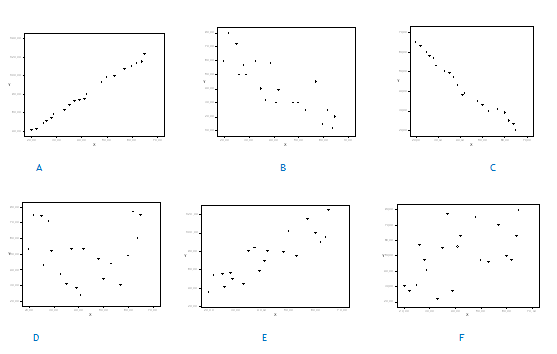
\includegraphics[width=\textwidth]{images/correlaties.png}
  \caption{Scatter plots of six data sets.}
\label{fig:correlations}
\end{figure}

\begin{exercise}
  \label{ex:cats-regression-correlation}
  Read data file \emph{cats.csv}. Perform a linear regression analysis on variables body weight (\emph{Bwt}) and heart weight (\emph{Hwt}).
  
  \begin{enumerate}
  \item Draw a scatter plot of these variables.
  \item Calculate and draw the regression line.
  \item Calculate the covariance, correlation and determination coefficients.
  \item Interpret the values from the previous steps.
  \end{enumerate}
\end{exercise}

\begin{exercise}
  Using the same data as in Exercise~\ref{ex:cats-regression-correlation}, perform a linear regression analysis on variables body weight (\emph{Bwt}) and heart weight (\emph{Hwt}) \emph{subdivided by gender} (\emph{Sex})
  
  \begin{enumerate}
  \item Draw scatter plots for the data.
  \item Calculate the regression lines.
  \item Calculate the covariance, correlation and determination coefficients.
  \item Interpret the values from the previous steps.
  \end{enumerate}
\end{exercise}

%\begin{exercise}
%  Read data file \emph{pizza.csv}. 
%  
%  \begin{enumerate}
%  \item Perform a complete regression analysis on variables \emph{Rating} and \emph{CostPerSlice}. Draw conclusions and check them by visualising the data.
%  \item Check whether there is a relation between \emph{Rating} and \emph{Neighbourhood}. What method can be used for this? Can you use the values of \emph{Rating} in their ``raw'' form?
%  \item Interpret your results.
%  \item Plot a graphical representation of the contingency table with a clustered bar chart.
%  \end{enumerate}
%\end{exercise}
%\chapter{The \texorpdfstring{$\chi^{2}$}{Chi-squared} test}
\label{chap:chisquared}

%\section{\texorpdfstring{$\chi^{2}$}{Chi-squared} test for distributions}
%
%Wanneer alle variabelen in het onderzoek nominaal zijn, is chi kwadraat de eenvoudigste (en populairste) techniek die men ter beschikking heeft voor het toetsten van hypothesen. De teststatistiek heet chi kwadraat, en is verdeeld volgens de chi kwadraat verdeling. De test kan gebruikt worden om na te gaan in welke mate de steekproef overeenstemt met een nulhypothese over de verdeling van de variabele. Men noemt dit een \textit{goodness of fit} \index{Test goodness of fit} test.
%
%In het voorbeeld op de slides willen we nagaan, of de verdeling van onze steekproef bij $n = 400$ superhelden overeenstemt met de verdeling die je verwacht in de volledige populatie (de verzameling van alle mogelijke superhelden). 
%
%Daartoe vergelijken we de aantallen in de steekproef met de aantallen die je zou verwachten als de steeproef exact representatief zou zijn naar de types van superhelden. Als deze verschillen relatief groot zijn dan komt de verdeling in de steekproef niet overeen met de verdeling in de populaties en zullen we moeten concluderen dat de steekproef niet representatief is. Om te oordelen of deze verschillen relatief groot zijn voeren we een $\chi^{2}$toets uit. 
%
%
%\subsection{Voorbeeld superhelden}
%We willen kijken of de steekproef voor onze superhelden representatief is. Als de steekproef exact representatief zou zijn zouden we verwachten dat in de steekproef 35\% van de superhelden een mutant zou zijn. Het verwachte aantal of de verwachte frequentie voor deze categorie is dus gelijk aan $0,35 \times 400 = 140$. De verwachte frequenties worden genoteerd met de letter $e$ (expected). Er geldt dus:
%
%\[ e = n \times \pi \]
%
%met $\pi$ de frequentie over de hele populatie. Als de verschillen $o - e$ ($o$ staat voor observed) reletief klein zijn kunnen ze toegerekend worden aan toevallige steekproeffouten. We gaan nu een toetsingsgrootheid bepalen waarmee getoetst kan worden of de steekproefverdeling overeenkomt met de gegeven verdeling in de populatie.
%
%Beschouw $\chi^{2}$:
%
%\[ \chi^{2} = \sum_{i=1}^{n} \frac{(o_{i} - e_{i})^{2}}{e_{i}} \]
%
%We merken op:
%\begin{itemize}
%	\item indien de verschillen klein zijn $\Rightarrow$ verdeling komt voldoende overeen
%	\item indien de verschillen groot $\Rightarrow$ verdeling niet representatief
%\end{itemize}
%
%We bepalen nu een kritieke grenswaarde $g$ die een $\chi^{2}$ verdeling heeft. Hierbij speel het aantal vrijheidsgraden een rol ($df$). Er geldt:
%
%\[ df = k -1 \]
%
%met $k$ het aantal categorie\"en. In ons voorbeeld hebben we $df = 5-1 = 4$. Om de kritieke grenswaarde te bepalen, kan je gebruik maken van een tabel voor de $\chi^2$-verdeling. Voor een gegeven significantieniveau $\alpha$ en vrijheidsgraad $df$ kan je in zo'n tabel de grenswaarde aflezen.
%
%In ons voorbeeld is $\chi^{2} = 3,47$ met grenswaarde $g = 9,49$. Omdat de gevonden toetsingsgrootheid $\chi^2 = 3,47 < g = 9,49$, mogen we besluiten dat de steekproef representatief is.
%
%
%\subsection{Toetsingsprocedure}
%We gaan ons 5-stappenplan invullen.
%
%\begin{enumerate}
%	\item \textbf{Bepalen hypotheses}
%		Als nulhypothese formuleren we dat de verdeling over de opleidingen in de steekproef gelijk is aan de verdeling in de populatie. Als alternatieve hypothese formuleren we dat de verdelingen verschillend zijn.
%		\begin{itemize}
%			\item $H_{0}$: steekproef is representatief naar populatie
%			\item $H_{1}$: steekproef is niet representatief naar populatie
%		\end{itemize}
%	\item \textbf{Bepalen $\alpha$ en $n$} : $\alpha = 0,05$ en $n = 400$.
%	\item \textbf{Toetsingsgrootheid en waarde ervan in steekproef}:
%	\[ \chi^{2} = \sum_{i=1}^{n} \frac{(o_{i} - e_{i})^{2}}{e_{i}} \]
%	\item \textbf{Bereken en teken kritiek gebied}: de toets is altijd rechtszijdig. Is de toetsingsgrootheid kleiner dan kritieke grenswaarde verwerp $H_{0}$ niet, anders verwerp $H_{0}$ en aanvaard $H_{1}$. 
%\end{enumerate}
%
%\subsection{Voorbeeld 2}
%
%Beschouw alle gezinnen met 5 kinderen in een bepaalde gemeenschap. Met betrekking tot samenstelling zijn er 6 mogelijkheden. 
%\begin{enumerate}
%	\item 5 jongens
%	\item 4 jongens, 1 meisje
%	\item 3 jongens, 2 meisjes
%	\item 2 jongens, 3 meisjes
%	\item 1 jongen, 4 meisjes
%	\item 5 meisjes
%\end{enumerate}
%
%Het onderzoek bevat 1022 gezinnen met 5 kinderen en resultaten staan beschreven in de slides (kolom = aantal jongens). Zijn de waargenomen aantallen in de 6 klassen representatief voor een populatie waar de kans om een jongen te krijgen = kans om een meisje te krijgen = 0,5?
%
%Indien de veronderstelling waar is wordt de kans $\pi_{i}$ om $i$ jongens te krijgen bepaald door een binominaalvedeling met parameters $n=5$ en $p=0,5$.
%
%Dit kan je eenvoudig nagaan aan de hand van voorbeeld. De kans om 2 jongens te krijgen met 5 kinderen is gelijk aan :
%
%\[ (0,5)^{2} \times (1-0,5)^{5-2} \times \binom{5}{2} \]
% 
%Algemeen geldt dus:
%
%\[ \pi_{i} = \binom{5}{i}\times 0,5^{i} \times 0,5^{5-i} = \frac{5!}{i!(5-i)!}\times 0,5^{i} \]
%
%Met deze $\pi_{i}$ kunnen we dus de verwachte waarde bepalen en de stappen volgen zoals hierboven beschreven. 
%
%\begin{enumerate}
%	\item \textbf{Bepalen hypotheses}
%		
%		\begin{itemize}
%			\item $H_{0}$: steekproef is representatief naar populatie
%			\item $H_{1}$: steekproef is niet representatief naar populatie
%		\end{itemize}
%	\item \textbf{Bepalen $\alpha$ en $n$} : $\alpha = 0,01$ en $n = 1022$.
%	\item \textbf{Toetsingsgrootheid en waarde ervan in steekproef}:
%	\[ \chi^{2} = \sum_{i=1}^{n} \frac{(o_{i} - e_{i})^{2}}{e_{i}} = 29,5766 \]
%	\item \textbf{Bereken en teken kritiek gebied}:  kritieke grens is 15,0863. Onze toetsingsgrootheid ligt dus in het kritieke gebied dus verwerpen we $H_{0}$. 
%\end{enumerate}
%
%We vinden dus dat de steekproef niet representatief is naar een populatie waar geldt dat de kans op een jongen even groot is als de kans op een meisje. Het is interessant om te kijken naar de gestandaardiseerde residuen die aanduiden welke klassen de grootste bijdrage leveren aan de waarde van de grootheid. 
%
%\[ r_{i} = \frac{O_{i} - n \pi_{i}}{\sqrt{n \pi_{i}(1-\pi_{i})}} \]
%
%\begin{exercise}
%	Hoe komen we hier aan de noemer? Waar komt dit mee overeen? Hoe bepaal je de variantie van een binomiale verdeling?
%Antwoord: $n \times \pi (1-\pi)$
%\end{exercise}
%
%
%
%Er geldt algemeen dat waarden groter dan 2 of kleiner dan $-2$ extreem zijn. We kunnen dus besluiten dat het aantal gezinnen waarin alle kinderen hetzelfde geslacht hebben groter mag worden genoemd dan verwacht.
%
%\subsection{Voorwaarden}
% Om de toets te mogen toepassen dient aan de volgende voorwaarden te zijn voldaan (Regel van Cochran)
%\begin{enumerate}
%	\item Voor alle categorie\"en moet gelden dat de verwachte waarde $e$ groter is dan 1.
%	\item In ten hoogste 20 \% van de categori\"en mag de verwachte waarde $e$ kleiner dan 5 zijn.
%\end{enumerate}
%
%
%\section{\texorpdfstring{$\chi^{2}$}{Chi-kwadraat}-kruistabeltoets}
%De Chi-kwadraattoets \index{$\chi^{2}$kwadraatkruistabeltoets} laat zich eenvoudig uitbreiden tot een onderzoeksontwerp
%met twee variabelen, met respectievelijk $r$ en $k$ niveaus. Hier gaan we onderzoeken of er een verband is tussen 2 variabelen. De procedure kan opnieuw geformuleerd worden.
%
%We gaan de procedure na aan de hand van een studie door \textcite{Doll1954} over de relatie tussen roken en longkanker. Doll en Hill schreven in 1951 alle Britse huisartsen aan met het verzoek om gegevens over hun leeftijd en rookgedrag. Vervolgens hielden ze jarenlang de overlijdensberichten en de doodsoorzaak bij en herhaalden hun periodiek. De eerste uitkomsten, na circa vier jaar, zijn in tabel~\ref{tab:dollhill} samengevat. Uit de tabel kan makkelijk geconcludeerd worden dat er geen relatie is tussen roken en longkanker. In (ruim) vier jaar is slechts $(84 / 24354) * 100 = 0,35\% $ van de Britse artsen aan longkanker overleden en dat met slechts $(83 / 21261) * 100 = 0,39\%$ van de rokers onder hen. Dit is weinig, maar het is wel veel meer dan hetzelfde cijfer voor de niet-rokers $(1 / 3093) * 100 = 0,032\%$.
%
%
%\begin{table}
%  \begin{center}
%    \begin{tabular}{@{}lllll@{}}
%      \toprule
%                       & \textbf{Longkanker} & \textbf{Niet} & \textbf{Wel} & \textbf{Totaal} \\
%        \midrule
%        \textbf{Roker} & \textbf{Wel}        & 21178         & 83           & 21261           \\
%                       & \textbf{Niet}       & 3092          & 1            & 3093            \\
%                       & \textbf{Totaal}     & 24270         & 84           & 24354           \\
%        \bottomrule
%    \end{tabular}
%  \end{center}
%  \caption{Resultaten van het onderzoek van~\textcite{Doll1954}}
%  \label{tab:dollhill}
%\end{table}
%
%We zien in de tabel dat er wel een erg groot verschil is tussen de geobserveerde aantallen rokers die overlijden aan longkanker en de verwachte waarden in deze cel. Hetzelfde geldt voor het geringe aantal huisartsen dat niet rookt, maar wel aan longkanker overleden is. Deze observatie maakt ons wel wantrouwig of de eerdere tentatieve conclusie wel juist is. We kunnen om aan deze onzekerheid de toetsingsgrootheid $\chi^{2}$ uitrekenen. Dat doen we op de vertrouwde manier:
%
%
%\begin{enumerate}
%	\item \textbf{Bepalen hypotheses}	
%		\begin{itemize}
%			\item $H_{0}$: in de populatie is er geen samenhang tussen onafhankelijke en afhankelijke variabele
%			\item $H_{1}$: er bestaat wel een samenhang tussen de variabelen in de populatie
%		\end{itemize}
%	\item \textbf{Bepalen $\alpha$ en $n$} : $\alpha = 0,05$ en $n = 24354$.
%	\item \textbf{Toetsingsgrootheid en waarde ervan in steekproef}:
%	\[ \chi^{2} = \sum_{i=1}^{n} \frac{(o_{i} - e_{i})^{2}}{E_{i}} = 10,35 \]
%	\item \textbf{Bereken en teken kritiek gebied}:  kritieke grens is 3,8415 en aantal vrijheidsgraden $df = (r-1)(k-1)$ Onze toetsingsgrootheid ligt dus in het kritieke gebied dus verwerpen we $H_{0}$. 
%\end{enumerate}
%
%We moeten derhalve $H_{0}$, dat er geen relatie is tussen beide variabelen, verwerpen ten gunste van $H_{1}$ dat er wel een relatie is tussen beide variabelen: rokers sterven vaker aan longkanker dan niet-rokers.
%
%Maar, is dit nu een bewijs dat zoals zo vaak verondersteld wordt dat roken longkanker veroorzaakt? Nee, dat is het absoluut niet. Een paar alternatieve verklaringen: niet alle rokers krijgen longkanker, de rokers zijn ouder dan de niet-rokers, de rokers wonen veelal in de grote steden met
%meer vervuilde lucht dan de niet-rokers die veelal op het platte land wonen, ook zo erg nog een speciale genetische dispositie kunnen zijn, die zowel van invloed is op de verslaving aan tabak, als op de kans om longkanker te krijgen. Voor een causale interpretatie van de gegevens (let wel, het betreft hier immers geen experiment), moeten we op zijn minst de beschikking hebben over een theorie die de relatie tussen roken en longkanker expliciteert.
%
%\subsection{Voorwaarden}
%Aan het voorwaarden van de $\chi^{2}$-kruistabeltoest zijn voorwaarden verbonden (regel van Cochran).
%\begin{enumerate}
%	\item Voor alle cellen moet gelden dat de verwachte waarde $e$ groter is dan 1.
%	\item in ten hoogste 20\% van de cellen mag de verwachte waarde $e$ kleiner zijn dan 5.
%\end{enumerate}
%


\section{Exercises}
\label{sec:chi-squared-exercises}

\begin{exercise}
  \label{ex:chisq-survey}
  This exercise makes use of the dataset \texttt{survey} that is included in R. The set contains results of a survey among students. In order to load the dataset, issue the following commands:
  
  \begin{lstlisting}
  library(MASS)
  View(survey)  # Show the "survey" dataset
  ?survey       # Help-page for the dataset, explains the contents
  \end{lstlisting}
  
  If you get an error message when loading the library (first line), this means that the package \texttt{MASS} is not yet instsalled. You can do this with Tools > Install Packages; fill out the package name in the text field.
  
  We want to know whether there is a relation between some discrete (i.e.~nominal or ordinal) variables in this dataset. For each of the pairs of variables, perform the following steps:
  
\begin{enumerate}[label=(\alph*)]
    \item First, reflect on the outcome you expect for the given set of variables.
    \item Determine a contingency table for the two variables. The (suspected) independent variable comes first.
    \item Plot a graph of the data, e.g.~a clustered bar chart, stacked percentage bar chart, or a ``mosaic chart'' (simply with \texttt{plot(table(data\$col1, data\$col2))}).
    \item If you look at the chart, do you expect a high or low value of the $\chi^2$-statistic? Why?
    \item Calculate the $\chi^2$-statistic and the critical value $g$ (for significance level $\alpha = 0.05$)
    \item Calculate the $p$-value
    \item Do we need to accept the null hypothesis, or can we reject it? What does that exactly mean for the relation between the two variables?
  \end{enumerate}
  
  The variables to be researched are given below. The suspected independent variable is the first.
  
  \begin{enumerate}
    \item \texttt{Exer} (sport habit) and \texttt{Smoke} (smoking habit)
    \item \texttt{W.Hnd} (writing hand) and \texttt{Fold} (the hand on top when folding arms)
    \item \texttt{Sex} and \texttt{Smoke}
    \item \texttt{Sex} and \texttt{W.Hnd}
  \end{enumerate}
\end{exercise}

\begin{exercise}
  \label{ex:chisq-aids2}
  Load the dataset \texttt{Aids2} from the package \texttt{MASS} (see Exercise~\ref{ex:chisq-survey}) that contains data about 2843 patients diagnosed with AIDS in Australia before 1991. This dataset was discussed in detail by ~\textcite{Ripley2007}. Determine whether there is a relation between the variables (\texttt{Sex}) and the way the disease was transmitted (\texttt{T.categ}).
  
  \begin{enumerate}
    \item Follow the usual steps: calculate contingency table, visualise the data, calculate the $\chi^2$, $g$ and $p$-value ($\alpha = 0,05$), and formulate a conclusion.
    \item Determine the standardised residuals in order to determine which categories contain extreme values.
  \end{enumerate}
  
\end{exercise}

\begin{exercise}
  \label{ex:chisq-digimeter}
  
  Every year, Imec (formerly iMinds) performs a study on the use of digital technologies in Flanders, the Digimeter~\autocite{Vanhaelewyn2016}. In this exercise, we're going to check whether the sample of the Digimeter 2016 ($n = 2164$) is representative for the Flemish population with regards to the age categories of the participants.
  
  Table~\ref{tab:digimeter2016} gives the relative frequencies of the participants. The absolute frequencies for the different age categories of the Flemish population is summarised in Table~\ref{tab:leeftijd-vlaanderen}, and is also included in CSV-file \texttt{exercises/data/bestat-vl-ages.csv}.
  
  \begin{enumerate}
    \item The table with age categories of the Flemish population has more categories than those used in the Digimeter. Recalculate the frequencies so you get the same categories as used in the Digimeter. Tip: this will probably be easier in a spreadsheet than in R.
    \item In order to apply a goodness-of-fit test, you need the absolute frequencies of the observed values in the sample. Calculate those.
    \item Also calculate the expected percentages ($\pi_{i}$) from the population frequencies.
    \item Perform a goodness-of-fit test over the distribution of age categories in the sample of the Digimeter 2016. Is the sample representative for the Flemish population?
  \end{enumerate}
\end{exercise}

\begin{table}
  \caption{Relative frequencies of age categories of the participants in the iMec Digimeter 2016 and the Flemish population.}
  \label{tab:frequenties-leeftijden}
  \centering
  \begin{tabular}{cc}
    \textbf{Age group} & \textbf{Percentage} \\ \midrule
    15-19 & 6,6\% \\
    20-29 & 14,2\% \\
    30-39 & 15,0\% \\
    40-49 & 16,3\% \\
    50-59 & 17,3\% \\
    60-64 & 7,3\% \\
    64+   & 23,2\% \\
  \end{tabular}
  \subcaption{Percentage of participants in the iMec Digimeter 2016 ($n = 2164$), per age category. \autocite{Vanhaelewyn2016}}
  \label{tab:digimeter2016}
  
  \centering
  \begin{tabular}{cc}
    \textbf{Age group} & \textbf{Frequency} \\ \midrule
    –5            &     352017      \\
    5-9           &     330320      \\
    10-14          &     341303      \\
    15-19          &     366648      \\
    20-24          &     375469      \\
    25-29          &     387131      \\
    30-34          &     401285      \\
    35-39          &     409587      \\
    40-44          &     458485      \\
    45-49          &     493720      \\
    50-54          &     463668      \\
    55-59          &     413315      \\
    60-64          &     379301      \\
    65-69          &     299152      \\
    70-74          &     279789      \\
    75-79          &     249260      \\
    80-84          &     182352      \\
    85-89          &     104449      \\
    90-94          &      29888      \\
    95-99          &      7678       \\
    100+           &       923
  \end{tabular}
  \subcaption{Absolute frequencies of the Flemish population per age category. Source: BelStat (\url{https://bestat.economie.fgov.be/bestat/}, C01.1: Bevolking volgens verblijfplaats (provincie), geslacht, positie in het huishouden (C), burgerlijke staat en leeftijd (B)).}
  \label{tab:leeftijd-vlaanderen}
  
  
\end{table}

\section{Solutions to selected exercises}
\label{sec:chi-squared-solutions}

\paragraph{Exercise~\ref{ex:chisq-survey}}

\begin{enumerate}
  \item \texttt{Exer}/\texttt{Smoke}: $\chi^2 = 5.49$, $g = 12.5916$, $p = 0.35$
  \item \texttt{W.Hnd}/\texttt{Fold}: $\chi^2 = 1.581399$, $g = 5.9915$, $p = 0.454$
  \item \texttt{Sex}/\texttt{Smoke}: $\chi^2 = 3.554$, $g = 7.8147$, $p = 0.314$
  \item \texttt{Sex}/\texttt{W.Hnd}: $\chi^2 = 0.236$, $g = 3.8415$, $p = 0.627$
\end{enumerate}

\paragraph{Exercise~\ref{ex:chisq-aids2}} $\chi^2 = 1083.372914$, $g = 14.067140$, $p \approx 1.157 \times 10^{-229}$

\paragraph{Exercise~\ref{ex:chisq-digimeter}} $\chi^2 = 6.6997$, $g = 12.5916$, $p = 0.35$
%\chapter{Time series}
\label{ch:time-series}

%\section{Tijdreeksen \& voorspellingen}
%
%\begin{definition}[Tijdsreeks]
%	Een tijdreeks is een opeenvolging van observaties van een willekeurige variabele in functie van de tijd.
%\end{definition}
%
%Een tijdreeks is dus eens stochastisch proces. Denk hierbij maar aan:
%\begin{itemize}
%	\item maandelijkse vraag naar melk
%	\item jaarlijkse instroom van studenten bij de Hogeschool
%	\item dagelijks debiet van een rivier
%\end{itemize}
%
%Het voorspellen van tijdreeksen is een belangrijk onderdeel van onderzoek omdat ze vaak de basis vormen voor beslissingsmodellen. Voorbeelden hiervan zijn :
%
%\begin{itemize}
%	\item algemene ontwikkeling van toekomstplannen (investeringen, capaciteit \dots)
%	\item plannen van budgettering om tekortkomingen te vermijden (operationeel budget, marketing budget \dots)
%	\item competitieve leveringstijden te bezorgen van een bedrijf
%	\item ondersteuning van financi\"ele objectieven
%	\item onzekerheid vermijden
%	\item de mogelijkheid om ontwikkelingen in de verkeersveiligheid
%kwantitatief te modelleren
%\end{itemize}
%
%Tijdreeksen modelleren is een statistisch probleem: we gaan ervan uit dat de observaties vari\"eren volgens een bepaalde kansdichtheidsfunctie in functie van de tijd. 
%
%Er zijn verschillende types modellen in gebruik voor het analyseren van tijdreeksen. Deze modellen hebben met elkaar gemeen dat ze in principe niet alleen de ontwikkeling in een geobserveerde tijdreeks kunnen beschrijven, maar dat we ze ook kunnen gebruiken om verklaringen voor de ontwikkeling in een geobserveerde tijdreeks te vinden, en om de toekomstige waarden van de
%ontwikkeling in een geobserveerde tijdreeks te voorspellen. Hun geschiktheid voor het verwezenlijken van deze doelstellingen loopt echter sterk uiteen. In dit hoofdstuk beperken we ons tot het gebruik van tijdreeksen met een geschiedenis om tijdsafhankelijke modellen te bepalen. 
%
%\section{Tijdreeksmodellen}
%\subsection{Wiskundig model}
%Ons doel is het opstellen van een model dat een verklaring vindt voor de geobserveerde data en dat toelaat om observaties in de toekomst zo goed mogelijk te voorspellen. Het simpelste model dat je kan bedenken is een model waarbij een constante $b$ gebruikt wordt met variaties rond $b$ bepaald door een willekeurige variabele $\epsilon_{t}$ zoals in vergelijking \ref{eq:constante}. 
%
%\begin{equation}
%	X_{t} = b + \epsilon_{t}
%\label{eq:constante}
%\end{equation}
%
%\begin{description}
%	\item [$X_{t}$] stelt een random variabele voor dat de onbekende is op tijdstip $t$.
%	\item [$x_{t}$] stelt een observatie voor op tijdstip $t$ (en is dus gekend). 
%	\item [$\epsilon_{t}$] noemt met de \textit{storing} (engels \textsl{noise}) en wordt geacht een gemiddelde van $0$ te hebben met variantie $\sigma^{2}$ en normaal verdeeld. 
%\end{description}
%
%\begin{figure}[htbp]
%	\centering
%		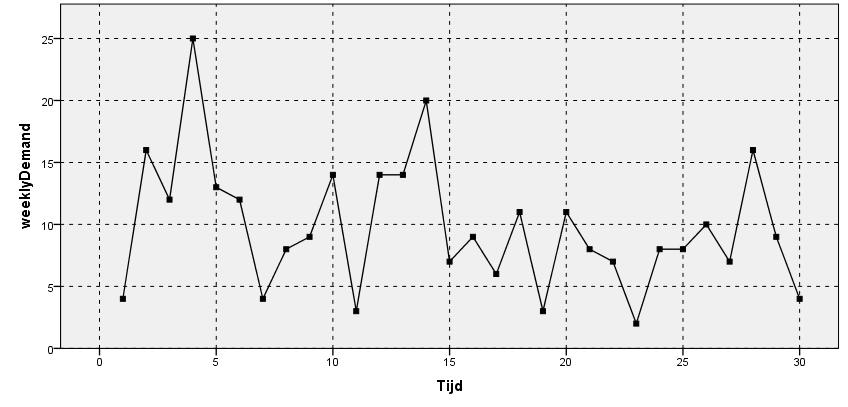
\includegraphics[width=\textwidth]{images/tijdsreeksen/tijdsreeks11.jpg}
%	\caption{Een tijdreeks voor een wekelijkse vraag voor een bepaald product}
%	\label{fig:tijdreeks11}
%\end{figure}
%
%
%We kunnen ook ervan uit gaan dat er een lineair verband is:
%
%\begin{equation}
%	X_{t} = b_{0} + b_{1} \times t + \epsilon_{t}
%\label{eq:lineair8}
%\end{equation}
%
%De vergelijking in \ref{eq:constante} en \ref{eq:lineair8} zijn speciale gevallen van het polynomiaal geval:
%
%\begin{equation}
%	X_{t} = b_{0} + b_{1} t + b_{2} t^{2} + \dots + b_{n} t^{n} + \epsilon_{t} 
%\label{eq:polynomiaal}
%\end{equation}
%
%\begin{exercise}
%	Wat zou volgende tijdreeks kunnen voorstellen?
%	\begin{equation}
%		X_{t} = b_{0} + b_{1} \sin(\frac{2\pi t}{4}) + b_{1} \cos(\frac{2\pi t}{4}) + \epsilon_{t}
%	\label{eq:seasonal}
%\end{equation}
%\end{exercise}
%
%Antwoord: dit is een cyclische tijdreeks met periode $= 4$. Dit zou bijvoorbeeld kunnen gebruikt worden bij een tijdreeks voor seizoenen.
%
%\subsubsection{Algemeen}
%
%In elk model beschouwd is de tijdreeks een functie van tijd en parameters van het model. We kunnen algemeen stellen dat:
%
%\begin{equation}
%	X_{t} = f(b_{0}, b_{1}, b_{2}, \dots , b_{t}, t) + \epsilon_{t}
%\label{eq:general}
%\end{equation}
%
%We aanvaarden vervolgens nog volgende stellingen:
%\begin{itemize}
%	\item Het model gaat uit van twee componenten van variabiliteit: het gemiddelde van de voorspellingen verandert met de tijd en de variaties tot dit gemiddelde vari\"eren willekeurig.
%	\item De residuen van het model ($X_{t} - x_{t}$) zijn homoscedastisch : dat wil zeggen in de tijd een constante variantie hebben.
%\end{itemize}
%
%Eenmaal het model gekozen, rest enkel nog het  probleem van het schatten van de parameters voor vergelijking \ref{eq:general}. Dit is wat in de volgende stukken besproken zal worden.
%
%\section{Schatten van de parameters}
%Eenmaal een model geselecteerd wordt, is het aan de onderzoeker om de parameters te gaan schatten, i.e. parameters die ervoor zorgen dat het model de geobserveerde waarden zo goed mogelijk benaderen. Meestal gaan we ervan uit dat alle waarden gelijkwaardig zijn, maar dat is niet zo bij tijdreeksen. Aangezien onze onafhankelijke parameter de tijd is moeten we methoden bekomen die ervoor zorgen dat recentere data belangrijker zijn dat oude data. 
%
%In wat volgt beschrijven we de tijdreeksen met geschatte waarden voor de parameters. We zetten hievoor een hoedje op de parameters:
%
%\[ \widehat{b}_{1}, \widehat{b}_{2} \dots \widehat{b}_{n} \] 
%
%Het schatten van de variatie voor $\sigma_{\epsilon}$ duiden we aan als $\widehat{\sigma}_{\epsilon}$.
%
%\subsection{Voorbeeld - moving average}
%
%\begin{table}[t]
%\centering
%    \begin{tabular}{|l|l|l|l|l|l|l|l|l|l|}
%    \hline
%    4 & 16 & 12 & 25 & 13 & 12 & 4 & 8  & 9 & 14 \\ \hline
%    3 & 14 & 14 & 20 & 7  & 9  & 6 & 11 & 3 & 11 \\ \hline
%    8 & 7  & 2  & 8  & 8  & 10 & 7 & 16 & 9 & 4  \\ \hline
%    \end{tabular}
%		\label{tab:data}
%		\caption{Voorbeeld data van vraag voor product, zie figuur \ref{fig:tijdreeks11}}
%\end{table}
%
%Stel dat de statisticus de data in tabel \ref{tab:data} tot het twintigste datapunt beschikbaar heeft (bekende data). De onderzoeker kent de datapunten vanaf het twintigste datapunt niet en moet deze gaan voorspellen. Een eerste model dat gebruikt zou kunnen worden is het constante model zoals in \ref{eq:constante}. 
%
%Met dit model, zijn de waarden random waarden uit een populatie met gemiddelde $b$. De beste schatter voor $b$ is het gemiddelde van deze twintig data punten. 
%
%\[ \widehat{b} = \frac{1}{20} \sum_{1}^{20} x_{t}= 10.75 \] 
%
%Dit is de beste schatter vertrekkende van de 20 datapunten. We merken wel op dat $x_{1} =  4$ evenveel waarde heeft als $x_{20} = 11$. 
%
%Indien we dit als schatter zouden gebruiken dan zien we dat dit in figuur \ref{fig:tijdreeks21} geen goed idee is.
%
%\begin{figure}[htbp]
%	\centering
%		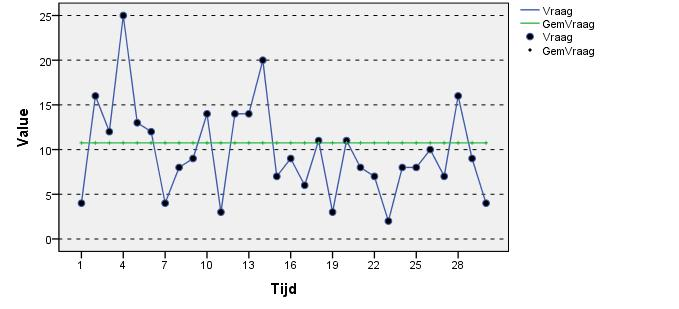
\includegraphics[width=1.00\textwidth]{images/tijdsreeksen/tijdsreeks21.jpg}
%	\caption{Tijdreeks met constant gemiddelde}
%	\label{fig:tijdreeks21}
%\end{figure}
%
%
%Indien we veronderstellen dat de data verandert met de tijd is het beter om oude data minder waarde te geven en de recente data meer waarde. Een mogelijkheid is om enkel recente data te gebruiken, bijvoorbeeld de 10 (zie fig. \ref{fig:tijdreeks31}) en 5 laatste datapunten (zie figuur \ref{fig:tijdreeks41}).
%
%\[ \widehat{b} = \frac{1}{10} \sum_{10}^{20} x_{t} = 10.18 \] en
%\[ \widehat{b} = \frac{1}{5} \sum_{15}^{20} x_{t} = 7.83 \]
%
%\begin{figure}
%	\centering
%		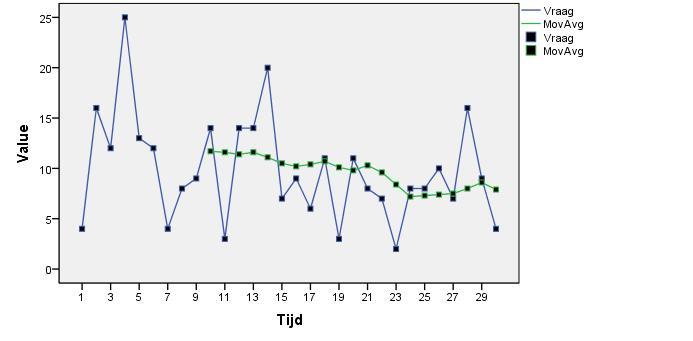
\includegraphics[width=1.00\textwidth]{images/tijdsreeksen/tijdsreeks31.jpg}
%		\caption{Tijdreeks met moving average $m = 10$}. 
%	\label{fig:tijdreeks31}
%\end{figure}
%
%\begin{figure}
%	\centering
%		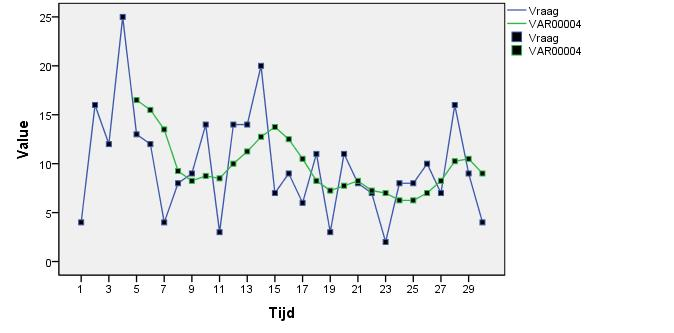
\includegraphics[width=1.00\textwidth]{images/tijdsreeksen/tijdsreeks41.jpg}
%	\caption{Tijdreeks met moving average $m = 5$}
%	\label{fig:tijdreeks41}
%\end{figure}
%
%
%
%Dit worden \textit{moving averages} genoemd \index{moving average}. 
%
%Welke schatter is nu de beste? We kunnen dit nu nog niet zeggen. 
%\begin{itemize}
%	\item De schatter die alle datapunten gebruikt is de beste indien de tijdreeks het model volledig volgt.
%	\item De schatter met de recentere datapunten is de beste indien de tijdreeks verandert met de tijd.
%\end{itemize}
%
%\begin{definition}
%	Algemeen is het moving average het gemiddelde van de $m$ laatste observaties.
%	\begin{equation}
%		\widehat{b} = \sum_{i=k}^{t} \frac{x_{i}}{m}
%	\label{eq:movingAverage}
%	\end{equation}
%	met $k = t-m+1$. $m$ is de time range en is de parameter van de methode.
%\end{definition}
%
%
%\begin{table}
%    \begin{tabular}{|lllllllllll|}
%    \hline
%    ~         & 11   & 12   & 13   & 14   & 15   & 16   & 17   & 18   & 19   & 20   \\
%    Data      & 3    & 14   & 14   & 20   & 7    & 9    & 6    & 11   & 3    & 11   \\
%    Schatting & 11.7 & 11.6 & 11.4 & 11.6 & 11.1 & 10.5 & 10.2 & 10.4 & 10.7 & 10.1 \\
%    Error     & -8.7 & 2.4  & 2.6  & 8.4  & -4.1 & -1.5 & -4.2 & 0.6  & -7.7 & 0.9  \\ \hline
%    \end{tabular}
%		\caption{Voorspellingsfout voor een moving average $m = 10$}
%		\label{tab:error}
%\end{table}
%
%\subsection{Meten van de nauwkeurigheid van voorspellingen}
%
%Een methode om de voorspelling te meten is het gemiddelde van de deviaties ($MAD$): gemiddelde absolute verschil tussen het voorspelde en de werkelijke waarden van de tijdsreeks.
%
%\begin{definition}[$MAD$]
%\begin{equation}
%	MAD = \frac{1}{n} \sum_{1}^{n} \left| e_{i} \right|  
%\label{eq:MAD}
%\end{equation}
%\end{definition}
%
%Je kan dit ook percenteren om zo tot de gemiddelde absolute procentuele afwijking ($MAPE$) te komen.
%
%\begin{definition}[$MAPE$]
%\begin{equation}
%	MAPE = \frac{1}{n} \sum_{1}^{n} \left| \frac{e_{i}}{X_i} \right|  
%\label{eq:MAD2}
%\end{equation}
%\end{definition}
%
%
%Je kan ook de variantie ervan bepalen:
%
%\begin{definition}[$VAR$]
%\begin{equation}
%	s^{2}_{e} = \frac{1}{m} \sum_{1}^{n} (e_{i} - \overline{e})^{2}
%\label{eq:varError}
%\end{equation}
%\end{definition}
%
%Als laatste interessante parameter kan gekeken worden naar de wortel uit de gemiddelde kwadratische afwijking ($RMSE$), als de wortel uit het gemiddelde kwadratische verschil tussen de voorspelde en de werkelijke waarden van de tijdsreeks.
%
%\begin{definition}[$RMSE$]
%\begin{equation}
%	RMSE_{e} = \sqrt{\frac{1}{m} \sum_{1}^{n} (e_{i})^{2}}
%\label{eq:varError2}
%\end{equation}
%\end{definition}
%
%
%\section{Exponenti\"ele smoothing}
%Bij een moving average krijgen alle voorgaande observaties een gelijk gewicht. Bij exponentieel smoothing worden kleinere gewichten toegekend aan oudere observaties. M.a.w.: recente observaties krijgen relatief meer gewicht dan oudere observaties.
%
%In het geval van moving average zijn de gewichten hetzelfde, namelijk $\frac{1}{m}$.
%
%\subsection{Enkelvoudige exponenti\"ele smoothing}
%Exponenti\"ele effening (of smoothing) is een gewogen gemiddlede dat positieve gewichten toekent aan de huidige waarden en waarden uit het verleden van de tijdsreeks. Een enkel gewicht, $0\leq \alpha \leq1$ of de exponentie\"ele effeningsconstante wordt hiervoor gekozen. 
%Voor een tijdseenheid $T$ wordt het enkelvoudige exponenti\"ele smoothing gevonden door vergelijking \ref{eq:singleExpSmooting}.
%
%\begin{definition}[Exponenti\"ele smoothing]
%\begin{equation}
%	X_{T} = \alpha x_{t-1} + (1-\alpha)X_{t-1}, 0 \leq \alpha \leq 1, t \geq 3
%\label{eq:singleExpSmooting}
%\end{equation}
%\end{definition}
%
%$\alpha$ wordt de smoothing constante genoemd.
%
%\subsubsection{Inti\"ele setting}
%Het bepalen van $X_{2}$ is een belangrijke parameter. Men kan kiezen om:
%\begin{enumerate}
%	\item $X_{2} = x_{1}$ te stellen
%	\item $X_{2}$ gelijk te stellen aan een bepaald objectief
%	\item Een gemiddelde te nemen van de eerste $x$ observaties
%	\item \dots
%\end{enumerate}
%
%\begin{exercise}
%	Waarom wordt dit een exponenti\"ele methode genoemd?
%\end{exercise}
%Antwoord: als we zouden substitueren vinden we bv. voor $X_{t-1}$:
%
%\[ X_{t} = \alpha x_{t-1} + (1-\alpha)\left[\alpha x_{t-2} + (1-\alpha)X_{t-2}\right] \] 
%\[ X_{t} = \alpha x_{t-1} + \alpha (1-\alpha)x_{t-2} + (1-\alpha)^{2} X_{t-2} \]
%of dus algemeen gesteld :
%\[ X_{t} = \alpha \sum_{i=1}^{t-2}(1-\alpha)^{i-1}x_{t-i} + (1-\alpha)^{t-2} X_{2}, t \geq 2 \]
%
%Zo merk je dat oudere componenten een exponentieel kleiner gewicht verkrijgen. 
%
%\subsubsection{Waarde voor $\alpha$}
%De snelheid waarmee de oude observaties ''vergeten`` worden hang af van $\alpha$. Met een $\alpha$ dicht bij 1 vergeet je snel, terwijl een $\alpha$ dicht bij nul ervoor zorgt dat vergeten minder snel gaat (zoals aangetoond in tabel \ref{tab:alpha}). Vaak wordt een waarde gebruikt tussen $0.10$ en $0.30$.
%
%\begin{table}
%\centering
%    \begin{tabular}{l|llll}
%    $\alpha$ & $(1-\alpha)$ & $(1-\alpha)^{2}$ & $(1-\alpha)^{3}$ & $(1-\alpha)^{4}$ \\ \hline
%    0.9   & 0.1       & 0.01             & 0.001                      & 0.0001           \\
%    0.5   & 0.5       & 0.25             & 0.125                      & 0.062            \\
%    0.1   & 0.9       & 0.81             & 0.729                      & 0.6561           \\
%    \end{tabular}
%		\caption{Waarden voor $\alpha$ en $(1-\alpha)^{n}$}
%		\label{tab:alpha}
%\end{table}
% 
%In figuur \ref{fig:tijdreeks51} vind je de tijdreeksen voor $\alpha=0.1 , 0.5, 0.9$.  
%
%\begin{figure}[htbp]
%	\centering
%		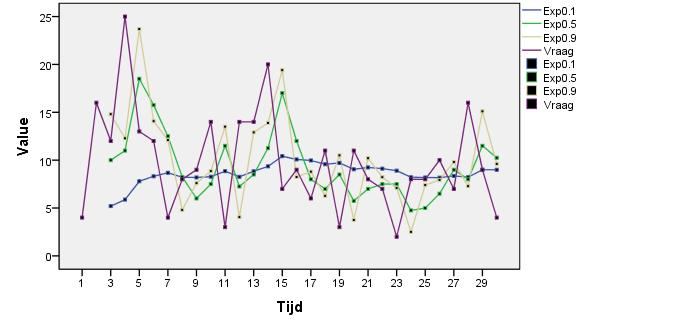
\includegraphics[width=1.00\textwidth]{images/tijdsreeksen/tijdsreeks51.jpg}
%	\caption{Enkelvoudig exponentieel model voor $\alpha=0.1 , 0.5, 0.9$}
%	\label{fig:tijdreeks51}
%\end{figure}
%
%\subsubsection{Voorspelling met exponenti\"ele effening}
%Stel dat het doel is om de volgende waarde $X_{t+1}$ te voorspellen, dan wordt dit gelijk gesteld aan de smoothing waarde op tijdstip $t$.
%
%\begin{equation}
%	X_{t+1} = EMA_t = X_t + \alpha(x_t - X_t)
%	\label{eq:EMA}
%\end{equation}
%
%\subsection{Dubbele exponenti\"ele smoothing}
%Enkelvoudige smoothing wordt gebruikt wanneer er geen trend zichtbaar is. Wanneer er een trend (stijgend of dalend) is dan kan er iets fout gaan. Zie bijvoorbeeld de data in tabel \ref{tab:trend} en figuur \ref{fig:tijdreeks61}.
%
%\begin{table}
%\centering
%    \begin{tabular}{|ll|}
%    \hline
%    Data & Enkelvoudige smoothing \\
%    6.4  & ~                      \\
%    5.6  & 6.4                    \\
%    7.8  & 6.2                    \\
%    8.8  & 6.7                    \\
%    11.0 & 7.3                    \\
%    11.6 & 8.4                    \\
%    16.7 & 9.4                    \\
%    15.3 & 11.6                   \\
%    21.6 & 12.7                   \\
%    22.4 & 15.4                   \\ \hline
%    \end{tabular}
%		\caption{Enkelvoudige smoothing met $\alpha = 0.3$}
%		\label{tab:trend}
%\end{table}
%
%\begin{figure}
%	\centering
%		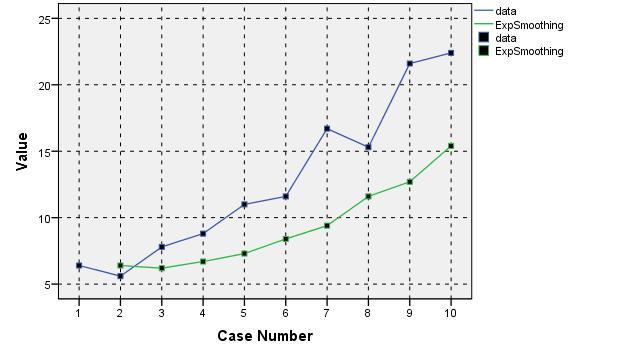
\includegraphics[width=1.00\textwidth]{images/tijdsreeksen/tijdsreeks61.jpg}
%	\caption{Exponenti\"ele smoothing bij een trend}
%	\label{fig:tijdreeks61}
%\end{figure}
%
%Daarom voegen we een extra constante toe om deze trap te overbruggen:
%
%\begin{definition}[Holt-voorspelling of dubbele exponenti\"ele voorspelling]
%\begin{eqnarray}
%	X_{t} = \alpha x_{t} + (1-\alpha)(X_{t-1} + b_{t-1}) & 0 \leq \alpha \leq 1 \\
%	b_{t} = \gamma(X_{t}-X_{t-1}) + (1-\gamma)b_{t-1} & 0 \leq \gamma \leq 1 
%\label{eq:doubleSmoothing}
%\end{eqnarray}
%\end{definition}
%
%\subsubsection{Initi\"ele waarde}
%Net zoals in enkelvoudige smoothing kan je verschillende methodes kiezen om initi\"ele waardes voor $X_{t}$ en $b_{t}$ te kiezen:
%\begin{itemize}
%	\item $X_{1} = x_{1}$
%	\item $b_{1} = x_{2} - x_{1}$
%	\item $b_{1} = \frac{1}{3}\left[ (x_{2} - x_{1}) + (x_{1} - x_{2}) + (x_{4} - x_{3}) \right]$
%	\item $b_{1} = \frac{x_{n} - x_{1}}{n-1}$
%\end{itemize}
%
%\subsubsection{Voorspelling}
%Een voorspelling maken met dubbele exponenti\"ele smoothing gebeurt dan iets anders (noem $F_{t+1}$ de voorspelling voor tijd $T+1$):
%
%\[ F_{t+1} = X_{t} + b_{t} \]
%of
%\[ F_{t+m} = X_{t} + m b_{t} \]
%
%Als we nu de tekening maken met enkelvoudige smoothing ($\alpha = 0.977$) en dubbele smoothing ($\alpha = 0.3623, \gamma = 1.0, X_{1} = x_{1} = 6.4$ en $b_{1} = \frac{1}{3}\left[ (x_{2} - x_{1}) + (x_{1} - x_{2}) + (x_{4} - x_{3}) \right] = 0.8$ vinden we volgende waarden in tabel \ref{tab:doubleSingle} en figuur \ref{fig:tijdreeks71}:
%
%\begin{table}
%\centering
%    \begin{tabular}{|llll|}
%    \hline
%    Data & Enkelvoudige smoothing $X_{t}$ & Double smoothing $X_{t}$ & $F_{t}$ \\
%    6.4  & ~                      & 6.4              & ~                             \\
%    5.6  & 6.4                    & 6.6              & 7.2                           \\
%    7.8  & 5.6                    & 7.2              & 6.8                           \\
%    8.8  & 6.7                    & 8.1              & 7.8                           \\
%    11.0 & 8.8                    & 9.8              & 9.1                           \\
%    11.6 & 10.9                   & 11.5             & 11.4                          \\
%    16.7 & 11.6                   & 14.5             & 13.2                          \\
%    15.3 & 16.6                   & 16.7             & 17.4                          \\
%    21.6 & 15.3                   & 19.9             & 18.9                          \\
%    22.4 & 21.5                   & 22.8             & 23.1                          \\ \hline
%    \end{tabular}
%		\caption{Tabel met enkelvoudige en dubbele smoothing}
%		\label{tab:doubleSingle}
%\end{table}
%
%\begin{figure}
%	\centering
%		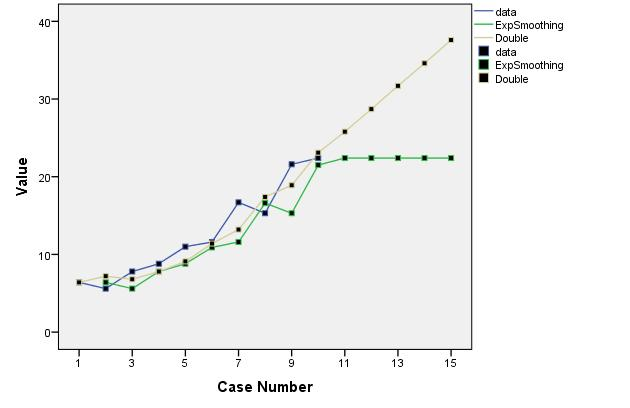
\includegraphics[width=1.00\textwidth]{images/tijdsreeksen/tijdsreeks71.jpg}
%	\caption{Enkelvoudige en dubbele smoothing}
%	\label{fig:tijdreeks71}
%\end{figure}
%
%\subsection{Driedubbele exponenti\"ele smoothing}
%Wanneer dubbele smoothing niet werkt kan driedubbele smoothing gebruikt worden, ofwel Holt-Winters methode genoemd.
%
%\begin{eqnarray}
%	X_{t} = \alpha \frac{x_{t}}{c_{t-L}} + (1-\alpha) (X_{t-1} + b_{t-1}) & \textnormal{Smoothing}\\
%	b_{t} = \gamma (X_{t} - X_{t-1}) + (1-\gamma)b_{t-1} & \textnormal{Trend smoothing} \\
%	c_{t} = \beta \frac{x_{t}}{X_{t}} + (1-\beta)c_{t-L} & \textnormal{Seasonal smoothing} \\
%	F_{t+m} = (X_{t} + mb_{t})c_{t-L+m} & \textnormal{Voorspelling}
%\label{eq:HoltWinters}
%\end{eqnarray}
% met 
%\begin{itemize}
%	\item $x_{t}$ de observatie op tijdstip $t$
%	\item $X_{t}$ is de smoothed observatie op tijdstip $t$
%	\item $b_{t}$ is de trendfactor op tijdstip $t$
%	\item $c_{t}$ is de seizoensindex op tijdstip $t$
%	\item $F_{t}$ is de voorspelling op tijdstip $t$
%	\item $L$ is de periode (bv. van de seizoenen)
%\end{itemize}
%
%$\alpha, \beta, \gamma$ zijn constanten die geschat moeten worden. 


\section{Exercises}
\label{sec:time-series-exercises}

\begin{exercise}
  In bijgevoegd bestand \texttt{exercises/time-series/budget.csv} vind je vanaf 1981 tot 2005 per kwartaal de omzet, het advertentiebudget en het BNP van een middelgroot bedrijf.  en voeg een kolom 'Kwartaalnummer' toe.
  \begin{enumerate}
    \item Bereken het voortschrijdend gemiddelde \emph{(simple moving average)} over de periodes 4 en 12 voor deze data. Gebruik hiervoor de methode SMA. Maak een lijngrafiek van $X$, $MA(4)$ en $MA(12)$.
    \item Welke techniek die we eerder gezien hebben (in het deel over beschrijvende statistiek) is ook geschikt om voorspellingen te maken over de waarden van $X$? Werk dit uit aan de hand van de daarvoor bestemde functie en plot het resultaat in de grafiek.
    \item Gebruik de methode \emph{forecast} om voorspellingen voor de 10 volgende periodes met elk van voorgaande methoden (dus moving average 4 en 10 en regressie) te maken. Teken deze eveneens op de grafiek.
    \item Is het gebruik van één van deze technieken interessant om voor deze data voorspellingen te maken? 
    \item Maak van de data een tijdreeks via de methode \emph{ts}. Gebruik de methode \emph{decompose} om de tijdreeks op te delen en zo een idee te krijgen van de trend en de seizoenschommeling.
    \item Bereken het exponentieel voortschrijdend gemiddelde \emph{(exponential moving average, EMA)} door gebruik te maken van de methode \emph{HoltWinters}. Maak opnieuw via de methode \emph{forecast} een voorspelling voor 20 periodes. Gebruik als startwaarden $s_1 = x_1$ en $\alpha $ de door R gegenereerde waarde. Plot het resultaat op een nieuwe grafiek samen met $X$.
    \item Doe nu hetzelfde met $\alpha=0.1$. 
    \item Hoe zien de voorspellingen er nu uit?
    \item Doe nu hetzelfde met \emph{dubbele} exponentiële afvlakking. Gebruik als startwaarden $s_1 = x_1$ en $b_1 = \frac{x_n - x_1}{n - 1}$, $\alpha =  0.05$ en $\beta = 0.2$. Plot het resultaat op de grafiek.
    \item Gebruik dubbele exponentiële afvlakking om voorspellingen te berekenen voor 20 periodes. Plot de waarden op de grafiek. Is deze techniek beter of slechter dan de vorige voor deze dataset?
    \item Speel met de waarden voor $\alpha$ en $\beta$ en bekijk het resultaat, zowel voor enkele als dubbele exponentiële afvlakking.
    \item Gebruik de \emph{HoltWinters}-methode zonder trend.  M.a.w. we stellen $\beta=0$. Gebruik als startwaarden $\alpha =  0.05$ en $\gamma = 0.9$. Plot het resultaat op de grafiek.
    \item Bereken opnieuw voorspellingen voor 20 periodes. Plot de waarden op de grafiek. Is deze techniek beter of slechter dan de vorige voor deze dataset?
    \item Speel met de waarden voor $\alpha$, $\beta$ en $\gamma$ en bekijk het resultaat.
    \item Gebruik de \emph{HoltWinters}-methode met de door R-gegeneerde waarden zonder trend.  M.a.w. we stellen $\beta=0$.  Plot het resultaat op de grafiek.
    \item Bereken opnieuw voorspellingen voor 20 periodes maar gebruik nu de methode \emph{predict}. Plot de waarden op de grafiek. Is deze techniek beter of slechter dan de vorige voor deze dataset?
  \end{enumerate}	
  
\end{exercise}

\begin{exercise}
  In bijgevoegd bestand \emph{exercises/time-series/passengers.csv} vind je vanaf januari 1949 tot december 1960 het aantal passagiers van een luchtvaartmaatschappij. 
  \begin{enumerate}
    \item Bereken het voortschrijdend gemiddelde \emph{(simple moving average)} over de periodes 4 en 12 voor deze data. Gebruik hiervoor de methode \emph{ma}. Maak een lijngrafiek van $X$, $MA(4)$ en $MA(12)$.
    \item Welke techniek die we eerder gezien hebben (in het deel over beschrijvende statistiek) is ook geschikt om voorspellingen te maken over de waarden van $X$? Werk dit uit aan de hand van de daarvoor bestemde functie en plot het resultaat in de grafiek.
    \item Gebruik de methode \emph{forecast} om voorspellingen voor de 10 volgende periodes met elk van voorgaande methoden (dus moving average 4 en 10 en regressie) te maken. Teken deze eveneens op de grafiek. Conclusie?
    \item Is het gebruik van één van deze technieken interessant om voor deze data voorspellingen te maken? 
    \item Gebruik de methode \emph{decompose} om de tijdreeks op te delen en zo een idee te krijgen van de trend en de seizoenschommeling.
    \item Bereken het exponentieel voortschrijdend gemiddelde \emph{(exponential moving average, EMA)} door gebruik te maken van de methode \emph{ses} met $\alpha=0.2$. Maak opnieuw via de methode \emph{forecast} een voorspelling voor 20 periodes. Plot het resultaat op een nieuwe grafiek samen met $X$.
    \item Doe nu hetzelfde met $\alpha=0.6$ en $\alpha=0.89$. 
    \item Hoe zien de voorspellingen er nu uit?
    \item Doe nu hetzelfde met \emph{dubbele} exponentiële afvlakking. Gebruik hiervoor de methode \emph{holt}  $\alpha =  0.8$ en $\beta = 0.2$. Plot het resultaat op de grafiek.
    \item Gebruik dubbele exponentiële afvlakking om voorspellingen te berekenen voor 20 periodes. Plot de waarden op de grafiek. Is deze techniek beter of slechter dan de vorige voor deze dataset?
    \item Gebruik in de methode de optie $exponential=TRUE$. Teken het resultaat.  Wat is het verschil?
    \item Gebruik de \emph{hw}-methode met de door R gegeneerde waarden. Plot het resultaat op de grafiek.
    \item Bereken opnieuw een aantal voorspellingen via de methode \emph{predict}. Plot de waarden op de grafiek. Is deze techniek beter of slechter dan de vorige voor deze dataset?
    \item Speel met de waarden voor $\alpha$, $\beta$ en $\gamma$ en bekijk het resultaat.
  \end{enumerate}
  
\end{exercise}	

\appendix

%\chapter{Notation}

\begin{table}
  \centering
  \begin{tabular}{p{.25\textwidth}p{.75\textwidth}}
    \toprule
    \textbf{Notation} & \textbf{Meaning} \\
    \midrule
    $X$                       & A stochastic variable \\
    $N$                       & The population size \\
    $n$                       & The sample size\\
    $\mu$ (mu)                & Population mean (also: expected value) \\
    $\overline{x}$            & Sample mean \\
    $\sigma$ (sigma)          & Population standard deviation \\
    $s$                       & Sample standard deviation \\
    $X \sim Nor(\mu, \sigma)$ & Variable $X$ is \emph{normally distributed} with mean $\mu$ and standard deviation $\sigma$ \\
    $Z \sim Nor(0, 1)$        & $Z$ is a variable with a distribution following the \emph{standard normal distribution}, i.e.~mean 0 and standard deviation 1 \\
    $M$                       & The probability distribution of the population mean, based on a sample (cfr.~the central limit theorem, Sectie~\ref{sec:central-limit-theorem}) \\

    \bottomrule
  \end{tabular}
\end{table}


\printbibliography
\addcontentsline{toc}{chapter}{\textcolor{maincolor}{\IfLanguageName{dutch}{Bibliografie}{Bibliography}}}

\end{document}
